%!TEX root = ../thesis_main.tex
%!TEX encoding = UTF-8 Unicode

%%%%%%%%%%%%%%%%%%%%%%%%%%%%%%%%%%%%%%%%%%%%%%%%%%%%%%%%%%%%%%%%%%%%
%%                                                                %%
%%                          PREAMBLE                              %%
%%                                                                %%
%%%%%%%%%%%%%%%%%%%%%%%%%%%%%%%%%%%%%%%%%%%%%%%%%%%%%%%%%%%%%%%%%%%%

%\documentclass[a4paper,twoside,10pt,draft]{memoir} %Compilation rapide
\documentclass[a4paper,twoside,10pt,final]{memoir} %Compilation lente

%!TEX encoding = UTF-8 Unicode
%!TEX root = ../thesis_main.tex


%%%%%%%%%%%%%%%%%%%%%%%%%%%%%%%%%%%%%%%%%%%%%%%%%%%%%%%%%%%%%%%%%%%%
%%                                                                %%
%%                        AUTHOR AND TITLE                        %%
%%                                                                %%
%%%%%%%%%%%%%%%%%%%%%%%%%%%%%%%%%%%%%%%%%%%%%%%%%%%%%%%%%%%%%%%%%%%%

\newcommand{\mytitle}{Robust optimisation of the pathway\texorpdfstring{\\ towards a sustainable whole-energy system}{}}
\newcommand{\mysubtitle}{A hierarchical multi-objective\texorpdfstring{\\ Reinforcement Learning-based approach}{}}
\newcommand{\myauthor}{Xavier Rixhon}

\def\eg{e.g.,\ }
\def\ie{i.e.,\ }
\def\og{``}
\def\fg{''}
\def\deg{$^{circ}$}


\usepackage[record,style=alttreegroup,nomain,symbols]{glossaries-extra}
\glsdisablehyper
%!TEX encoding = UTF-8 Unicode
%!TEX root = ../thesis_main.tex

%%%%%%%%%%%%%%%%%%%%%%%%%%%%%%
%	MATH SYMBOLS							%
%%%%%%%%%%%%%%%%%%%%%%%%%%%%%%

\glsxtrsetgrouptitle{Abreviation}{Abreviation}
\glsxtrsetgrouptitle{Notation}{Notation}

% \newcommand{\sdot}{{\bullet}}
\newcommand{\sdot}{(\cdot)}

% ---------------------------------------------------------------------------- %
% ACRONYMS
%% A

%% P
\newabbreviation[group={Acronyms}]{PCE}{PCE}{Polynomial Chaos Expansion}

%% S
\newabbreviation[group={Acronyms}]{SDGs}{SDGs}{Sustainable Development Goals}

%% U
\newabbreviation[group={Acronyms}]{UQ}{UQ}{Uncertainty Quantification}

% ---------------------------------------------------------------------------- %
% ROMAN
%% A
%\glsxtrnewsymbol[group={rs},description={ith ambient particle}]{ai}{\ensuremath{A_i}}


% ---------------------------------------------------------------------------- %
% GREEK
%\glsxtrnewsymbol[group={gs},description={Yaw angle [$\deg$]}]{beta}{\ensuremath{\beta}}


% ---------------------------------------------------------------------------- %
% Sub- Superscripts
%% A
%\glsxtrnewsymbol[group={ss},description={Relative to the ambient}]{uA}{\ensuremath{\sdot_{A}}}



\renewcommand\glstreegroupheaderfmt[1]{\begingroup\textbf{#1}\vspace{-.2cm}\par\endgroup}
\glsfindwidesttoplevelname
\glsxtrsetgrouptitle{Acronyms}{Acronyms}
\glsxtrsetgrouptitle{rs}{Roman Symbols}
\glsxtrsetgrouptitle{gs}{Greek Symbols}
\glsxtrsetgrouptitle{ss}{Sub- Superscripts}
\glsxtrsetgrouptitle{o}{Operators}

%------------------------
%% A
%\newcommand{\ABL}[2]{$U_\mABL=\SIms{#1}$ - $TI_\mABL={#2}\%$}
%------------------------
%% B

%------------------------
%% C

%------------------------
%% D
\newcommand{\degree}{^\circ}
\newcommand{\dd}{\mathrm{d}}

%------------------------
%% E
\newcommand{\etal}{\textit{et~al.}}
\newcommand{\eg}{e.g.\ }

%------------------------
%% F

%------------------------
%% G

%------------------------
%% H

%------------------------
%% I
\newcommand{\ie}{i.e.\ }

%------------------------
%% K

%------------------------
%% L

%------------------------
%% M

%------------------------
%% N

%------------------------
%% O

%------------------------
%% P

%------------------------
%% Q

%------------------------
%% R

%------------------------
%% S

%------------------------
%% T


%------------------------
%% U
\newcommand{\uh}{\hat{u}}
\newcommand{\uv}{\mathbf{u}} 

\newcommand{\ub}{\boldsymbol{u}} 

\newcommand{\uconvw}{\tilde{U}_W}

%------------------------
%% V
\newcommand{\vv}{\mathbf{v}}
\newcommand{\vb}{\boldsymbol{v}}

%------------------------
%% W
\newcommand{\wv}{\mathbf{w}}
\newcommand{\wb}{\boldsymbol{w}}
\newcommand{\WT}{{\scriptscriptstyle \mathrm{WT}}}

%------------------------
%% X
\newcommand{\xv}{\mathbf{x}}
\newcommand{\xb}{\boldsymbol{x}}

%------------------------
%% Y
\newcommand{\yv}{\mathbf{y}}
\newcommand{\yb}{\boldsymbol{y}}

%------------------------
%% Z
\newcommand{\zv}{\mathbf{z}}
\newcommand{\zb}{\boldsymbol{z}}

%%%%%%%%%%%%%%%%%%%%%%%%%%%%%%
%	OPERATORS 								%
%%%%%%%%%%%%%%%%%%%%%%%%%%%%%%
\newcommand{\der}[2]{\frac{d #1}{d #2}}
\newcommand{\pder}[2]{\frac{\partial #1}{\partial #2}}
\newcommand{\pdern}[3]{\frac{\partial^#3 #1}{\partial #2^#3}}

\newcommand{\avgt}[1]{\left\langle {#1}\right\rangle}
\newcommand{\avgs}[1]{\overline{#1}}

%%%%%%%%%%%%%%%%%%%%%%%%%%%%%%
%	REFERENCES 							%
%%%%%%%%%%%%%%%%%%%%%%%%%%%%%%

\newcommand{\eqqref}[1]{Eq.~\eqref{#1}}
\newcommand{\seqqref}[1]{Eqs.~\eqref{#1}}
\newcommand{\eqqrefs}[2]{Eqs.~\eqref{#1} and \eqref{#2}}
\newcommand{\eqqrefc}[2]{Eqs.~\eqref{#1}, \eqref{#2}}
\newcommand{\eq}[1]{Eq.~\eqref{#1}}
% \newcommand{\eqs}[1]{Eqs.~(\ref{#1})}

\newcommand{\fig}{Fig.~\ref}
\newcommand{\figs}{Figs.~\ref}
\newcommand{\tab}{Table~\ref}
\newcommand{\sect}{Section~\ref}
\newcommand{\chap}{Chapter~\ref}
\newcommand{\chaps}{Chapters~\ref}
\newcommand{\app}{Appendix~\ref}
\newcommand{\apps}{Appendices~\ref}

%%%%%%%%%%%%%%%%%%%%%%%%%%%%%%
%	CAPTIONS							%
%%%%%%%%%%%%%%%%%%%%%%%%%%%%%%
% Color palette
  
\usepackage{xcolor}
\definecolor{myBlue}{rgb}{0.25, 0.25, 0.75}
\definecolor{myRed}{rgb}{0.8, 0.1, 0.3}
\definecolor{myGrey0}{rgb}{0.25, 0.25, 0.25}
\definecolor{myGrey1}{rgb}{0.50, 0.50, 0.50}
\definecolor{myGrey2}{rgb}{0.75, 0.75, 0.75}


\definecolor{Blue0}{rgb}{0.7752402921953095, 0.8583006535947711, 0.9368242983467897}
\definecolor{Blue1}{rgb}{0.41708573625528644, 0.6806305267204922, 0.8382314494425221}
\definecolor{Blue2}{rgb}{0.1271049596309112, 0.4401845444059977, 0.7074971164936563}
\definecolor{Blue3}{rgb}{0.03137254901960784, 0.18823529411764706, 0.4196078431372549}

\definecolor{BluePy}{rgb}{0.69140625, 0.8164, 0.8868}
\definecolor{RedC}{rgb}{0.9453, 0.7266, 0.6602}

\definecolor{gw}{rgb}{1, 0, 0}
\definecolor{jb}{rgb}{0, 1, 0}
\definecolor{tg}{rgb}{0, 0, 1}
\definecolor{jh}{rgb}{1, 1, 0}

\newcommand{\gw}[1]{{#1}}
% \newcoxmmand{\gw}[1]{\textcolor{gw}{#1}}
\newcommand{\jb}[1]{\textcolor{jb}{#1}}
\newcommand{\tg}[1]{\textcolor{tg}{#1}}
\newcommand{\jh}[1]{\textcolor{jh}{#1}}


%%%%%%%%%%%%%%%%%%%%%%%%%%%%%%%%%%%%%%%%%%%%%%%%%%%%%%%%%%%%%%%%%%%%
%%                                                                %%
%%                       LANGUAGE AND FONTS                       %%
%%                                                                %%
%%%%%%%%%%%%%%%%%%%%%%%%%%%%%%%%%%%%%%%%%%%%%%%%%%%%%%%%%%%%%%%%%%%%

% -- Language ------------------------------------------------------
\usepackage[utf8]{inputenc}
\usepackage[USenglish]{babel}
\usepackage[T1]{fontenc} % Accents
\usepackage{scrextend} % to use \footref: multiple reference to the same table footnote
\usepackage{pbox} % to have new line inside table cells

% -- Fonts ---------------------------------------------------------
%\usepackage{lmodern}
%% utopia
%\usepackage{fourier}
%% palatino
%\usepackage{palatino}
%% pifont
%\usepackage{pifont}
%% charter
%\usepackage{charter}

% stix
\usepackage[lcgreekalpha]{stix}
\usepackage{textcomp}

%% better and newer palatino font
%\usepackage{newpxtext,newpxmath}

%% special font, no ams package included...
%\usepackage[full]{textcomp}
%\usepackage[osf]{newtxtext} % osf for text, not math
%\usepackage{cabin} % sans serif
%\usepackage[varqu,varl]{inconsolata} % sans serif typewriter
%\usepackage[bigdelims,vvarbb]{newtxmath} % bb from STIX
%\usepackage[cal=boondoxo]{mathalfa} % mathcal


%%%%%%%%%%%%%%%%%%%%%%%%%%%%%%%%%%%%%%%%%%%%%%%%%%%%%%%%%%%%%%%%%%%%
%%                                                                %%
%%                    TEXT, LAYOUT AND STRUCTURE                  %%
%%                                                                %%
%%%%%%%%%%%%%%%%%%%%%%%%%%%%%%%%%%%%%%%%%%%%%%%%%%%%%%%%%%%%%%%%%%%%

% -- Paragraphs---- ------------------------------------------------
\linespread{1.15}
%\usepackage[parfill]{parskip} %% NOT working with memoir class... see https://tex.stackexchange.com/questions/193485/how-to-use-usepackageparfillparskip-in-memoir-class for discussion

% -- Margins -------------------------------------------------------
\usepackage[includehead,includefoot,centering,height=20cm,width=12cm,showframe=false]{geometry}
%\usepackage[includehead,includefoot,centering,height=20cm,width=12cm,showframe=false]{geometry}

%\usepackage[includehead,includefoot,centering,height=20cm,width=12cm,showframe=true]{geometry} %taille des marges
%\usepackage[includehead, includefoot, top=4.2cm, bottom=5.4cm, left=4.5cm, right=4.5cm,showframe=true]{geometry}%…PhP
%\usepackage[includehead, includefoot, top=4.8cm, bottom=4.8cm, left=4.5cm, right=4.5cm,showframe=true]{geometry}%4.8 4.8

% -- Layout --------------------------------------------------------
%\usepackage{layout} % pour afficher le layout des pages

%\usepackage{color}
%\usepackage[dvipsnames]{xcolor}s
\usepackage{lineno}
%\usepackage{ulem} %underline for emphasis
\usepackage{fancyhdr}% pour en-tetes personnalises
\usepackage{appendix} % gestion appendix
\usepackage{tikz}% pour diagrammes
\usetikzlibrary{shapes.misc}
\usepackage{setspace}

%\usepackage{titlepages} % for the titlepage examples

%\usepackage{charter}
%\usepackage[raggedright]{titlesec} % evite les coupures de mot dans les titres

\usepackage{afterpage} % Force content to be on the next page

%% The lineno packages adds line numbers. Start line numbering with
%% \begin{linenumbers}, end it with \end{linenumbers}. Or switch it on
%% for the whole article with \linenumbers.
\usepackage{lineno} % Line numbers

\sloppy % evite les debordements de texte dans la marge
\raggedbottom %regroupe les espaces verticaux automatiques au bas des pages

% -- Structure et Paragraphes --------------------------------------
%evite les lignes veuves et orphelines
\clubpenalty=10000
\widowpenalty=10000
\interfootnotelinepenalty=10000

%\setcounter{secnumdepth}{3} % numerote les subsubsections
\setsecnumdepth{subsection}
\maxtocdepth{subsection}

% -- Style ---------------------------------------------------------
\normalfont
% chapter style
%\chapterstyle{ell}
%\chapterstyle{madsen}
%\chapterstyle{bianchi}
%\chapterstyle{dash}
%\chapterstyle{thatcher}
\newcommand{\clearemptydoublepage}{\newpage{\pagestyle{empty}\cleardoublepage}} %pour effacer les en-tetes sur la page vierge avant chaque chapitre

%\pagestyle{ruled}
\nouppercaseheads
\pagestyle{headings}
\makeheadrule{headings}{\textwidth}{0.3pt}


%%%%%%%%%%%%%%%%%%%%%%%%%%%%%%%%%%%%%%%%%%%%%%%%%%%%%%%%%%%%%%%%%%%%
%%                                                                %%
%%                     TABLES AND FIGURES                         %%
%%                                                                %%
%%%%%%%%%%%%%%%%%%%%%%%%%%%%%%%%%%%%%%%%%%%%%%%%%%%%%%%%%%%%%%%%%%%%

% -- Figures -------------------------------------------------------
\usepackage{graphicx}
\graphicspath{{frontend/img/}{chap_intro_ccl/img/}{chap_case_study/img/}{chap_ES_PCE/img/}{chap_electro_uq/img/}{chap_methodo/img/}{chap_myopic/img/}{chap_RL/img/}{chap_atom_mol/img/}{chap_RobPol/img/}{appendices/img/}} % Figures folder different for each input
%\graphicspath{{img/}} %
\DeclareGraphicsExtensions{.eps,.pdf,.png,.jpg}

%\usepackage[cleanup,process=auto]{pstool}
%\usepackage[cleanup,process=all]{pstool} % force process every figure
%\usepackage{pst-pdf}
%\usepackage{epstopdf}
%\usepackage{auto-pst-pdf} 
%\usepackage{psfrag}
%\PassOptionsToPackage{psfrag}{process=none}

\usepackage[figuresright]{rotating} %https://tex.stackexchange.com/questions/337/how-to-change-certain-pages-into-landscape-portrait-mode

\def\figwidth{0.9\textwidth}
\newcommand{\singlefigwidth}{.75\textwidth}

\setfloatadjustment{figure}{\centering}
\setfloatlocations{figure}{thb}
\newsubfloat{figure}

\newcommand{\illusname}{Illustration}
\newcommand{\listillusname}{List of Illustrations}
\newlistof{listofillus}{loillu}{\listdiagramname}
\newfloat[chapter]{illustration}{loillu}{\illusname}
\newlistentry{illustration}{loillu}{0}
\renewcommand\theillustration{\arabic{illustration}}    

\usetikzlibrary{shapes}

% -- Tables --------------------------------------------------------
\usepackage{booktabs} % Table customization: \specialrule

\usepackage{longtable} % Long tables on multiple pages
\usepackage{tabu}
\usepackage{ltablex} % Use ltablex instead of tabularx
\usepackage{multirow} % Cellule de tableau sur plusieurs lignes
\usepackage{multicol} % Cellule de tableau sur plusieurs colonnes
\usepackage{dcolumn} % Columns aligned on decimal point
\newcolumntype{d}[1]{D{.}{.}{#1}}
\usepackage{array} % ??

%\usepackage{cellspace} % Espace entre le texte et les bord des cellules
%\usepackage{tabularx} % Tableau avec largeur fixée

\usepackage{makecell} % Customize table headers with \thead
\renewcommand\theadfont{\bfseries} % Customize table column headers with \thead

% -- Sub-figures and Captions --------------------------------------
\usepackage{subfig}
\usepackage{wrapfig} % Images dans le texte
%\usepackage{floatrow} % Tableau et figure côte à côte
%\usepackage{subcaption} % sub caption

\usepackage[labelfont=bf, labelsep=period, justification=justified,singlelinecheck=false]{caption} % style et taille de police des captions
%\captionsetup[table]{position=below}

%\captionnamefont{\sffamily} % font for the "Figure xx" part
%\captionnamefont{\footnotesize\sffamily} % font for the "Figure xx" part
%\captionnamefont{\footnotesize} % font for the "Figure xx" part
%\captiontitlefont{\footnotesize} % font for the caption part
%\captiontitlefont{\small}
% change caption witdth
%\changecaptionwidth
%\captionwidth{0.9\textwidth}
%\captionstyle[\centering]{}


%%%%%%%%%%%%%%%%%%%%%%%%%%%%%%%%%%%%%%%%%%%%%%%%%%%%%%%%%%%%%%%%%%%%
%%                                                                %%
%%                      SCIENTIFIC PACKAGES                       %%
%%                                                                %%
%%%%%%%%%%%%%%%%%%%%%%%%%%%%%%%%%%%%%%%%%%%%%%%%%%%%%%%%%%%%%%%%%%%%

% -- Math ----------------------------------------------------------
\usepackage{amsmath}
%\usepackage[intlimits]{amsmath}
\usepackage{amsfonts}
\usepackage{amsthm} % Extended theorem environments
%\usepackage{amssymb} % Math symbols %%redundant with stix package
%\usepackage{esint} % Intégrales multiples
%\usepackage{esvect} % Vecteurs
\usepackage{mathtools}
\usepackage{pifont}

% Put the equation label in the document, to help writing
\usepackage{showlabels}
%\usepackage[final]{showlabels} %disable

\usepackage[boxed]{algorithm2e}

% -- Physics and Chemistry -----------------------------------------
\usepackage{siunitx} % SI units
\usepackage[version=4]{mhchem} % Chemical equations

% -- Symbols -------------------------------------------------------
\usepackage[super]{nth} %text superscript \nth{i}
\usepackage{textcomp} % Degree symbol °, and certainly others
%\newcommand{\cmark}{\ding{51}}
%\newcommand{\xmark}{\ding{55}}


%%%%%%%%%%%%%%%%%%%%%%%%%%%%%%%%%%%%%%%%%%%%%%%%%%%%%%%%%%%%%%%%%%%%
%%                                                                %%
%%                  BIBLIOGRAPHY AND HYPERREF                     %%
%%                                                                %%
%%%%%%%%%%%%%%%%%%%%%%%%%%%%%%%%%%%%%%%%%%%%%%%%%%%%%%%%%%%%%%%%%%%%

% -- Bibliography --------------------------------------------------
% For natbib help, see http://merkel.texture.rocks/Latex/natbib.php?lang=fr
%\usepackage{biblatex}
\usepackage[square,numbers,sort&compress]{natbib}
%\setlength{\bibsep}{0.5pt}
%\usepackage{pdfcomment}
%\usepackage[square,numbers,compress]{natbibtooltip}
\usepackage{textcomp} % recognize the textquotesingle from bib

\bibliographystyle{options/elsarticle-num-names}  %Ordered by appearance in the text, with DOI and URL

%\bibliographystyle{options/elsarticle-num}  %Same but \citet command does not work
%\bibliographystyle{options/elsarticle-harv}  %Harvard style (Author, year, no number)
%\bibliographystyle{options/elsarticle-num-names-nourldoi}  %Ordered by appearance in the text, with DOI
%\bibliographystyle{options/elsarticle-names-nourldoi}  %Ordered by alphabet, with DOI
%\bibliographystyle{options/elsarticle-names-nourl} %Ordered by alphabet, without DOI
%\bibliographystyle{options/model4-names}

% -- Hyperref ------------------------------------------------------
\PassOptionsToPackage{hyphens}{url} %this helps breaking URL when too long
\usepackage[bookmarks,hidelinks]{hyperref}
\usepackage{cleveref}
\usepackage{bm} % To use \bm in order to get bold math symbols

% PDF metadata
\hypersetup{pdftitle={\mytitle}}
\hypersetup{pdfauthor={\myauthor}}
\hypersetup{pdfsubject={PhD thesis}}
\hypersetup{pdfkeywords={Energy System Modelling,EnergyScope,Reinforcement Learning,Policy Optimisation, Electro-fuels}}

% Links color
\newcommand\myshade{85}
% from http://latexcolor.com
\definecolor{airforceblue}{rgb}{0.36, 0.54, 0.66}
\definecolor{battleshipgrey}{rgb}{0.52, 0.52, 0.51}
\definecolor{burntumber}{rgb}{0.54, 0.2, 0.14}
\definecolor{sangria}{rgb}{0.57, 0.0, 0.04}
\colorlet{mylinkcolor}{sangria}
\colorlet{mycitecolor}{battleshipgrey}

%\hypersetup{
%%linkcolor  = mylinkcolor!\myshade!black,
%%citecolor  = mycitecolor!\myshade!black,
%%urlcolor   = myurlcolor!\myshade!black,
%colorlinks = true,
%}

%\hypersetup{
%    colorlinks=true,
%    citecolor = blue,
%    linkcolor=blue,
%    urlcolor = blue
% }

%% Links with color frame
\hypersetup{
colorlinks = false,
%citebordercolor ={red},
}

%% No color on links (for printing)
%\hypersetup{hidelinks}

% Adding bookmarks to pdf (works after clearing aux and then 2 clean compilations)
%\hypersetup{bookmarks={true}} % --> does it by default

%% Reference with Fancy Tooltips (only works with the dedicated compilation script)
%from: https://tex.stackexchange.com/questions/84681/interactive-pdf-latex-and-article-of-the-future/84700#84700
%\usepackage[inactive,blur=0.6, fixcolor]{fancytooltips}
%\usepackage[inactive]{fancytooltips}

% -- Footnotes ------------------------------------------------------
\newcommand\blfootnote[1]{%
  \begingroup
  \renewcommand\thefootnote{}\footnote{#1}%
  \addtocounter{footnote}{-1}%
  \endgroup} %%Footnotes sans numéro

%%!TEX encoding = UTF-8 Unicode
%!TEX root = ../thesis_main.tex

%%%%%%%%%%%%%%%%%%%%%%%%%%%%%%
%	MATH SYMBOLS							%
%%%%%%%%%%%%%%%%%%%%%%%%%%%%%%

\glsxtrsetgrouptitle{Abreviation}{Abreviation}
\glsxtrsetgrouptitle{Notation}{Notation}

% \newcommand{\sdot}{{\bullet}}
\newcommand{\sdot}{(\cdot)}

% ---------------------------------------------------------------------------- %
% ACRONYMS
%% A

%% P
\newabbreviation[group={Acronyms}]{PCE}{PCE}{Polynomial Chaos Expansion}

%% S
\newabbreviation[group={Acronyms}]{SDGs}{SDGs}{Sustainable Development Goals}

%% U
\newabbreviation[group={Acronyms}]{UQ}{UQ}{Uncertainty Quantification}

% ---------------------------------------------------------------------------- %
% ROMAN
%% A
%\glsxtrnewsymbol[group={rs},description={ith ambient particle}]{ai}{\ensuremath{A_i}}


% ---------------------------------------------------------------------------- %
% GREEK
%\glsxtrnewsymbol[group={gs},description={Yaw angle [$\deg$]}]{beta}{\ensuremath{\beta}}


% ---------------------------------------------------------------------------- %
% Sub- Superscripts
%% A
%\glsxtrnewsymbol[group={ss},description={Relative to the ambient}]{uA}{\ensuremath{\sdot_{A}}}



\renewcommand\glstreegroupheaderfmt[1]{\begingroup\textbf{#1}\vspace{-.2cm}\par\endgroup}
\glsfindwidesttoplevelname
\glsxtrsetgrouptitle{Acronyms}{Acronyms}
\glsxtrsetgrouptitle{rs}{Roman Symbols}
\glsxtrsetgrouptitle{gs}{Greek Symbols}
\glsxtrsetgrouptitle{ss}{Sub- Superscripts}
\glsxtrsetgrouptitle{o}{Operators}

%------------------------
%% A
%\newcommand{\ABL}[2]{$U_\mABL=\SIms{#1}$ - $TI_\mABL={#2}\%$}
%------------------------
%% B

%------------------------
%% C

%------------------------
%% D
\newcommand{\degree}{^\circ}
\newcommand{\dd}{\mathrm{d}}

%------------------------
%% E
\newcommand{\etal}{\textit{et~al.}}
\newcommand{\eg}{e.g.\ }

%------------------------
%% F

%------------------------
%% G

%------------------------
%% H

%------------------------
%% I
\newcommand{\ie}{i.e.\ }

%------------------------
%% K

%------------------------
%% L

%------------------------
%% M

%------------------------
%% N

%------------------------
%% O

%------------------------
%% P

%------------------------
%% Q

%------------------------
%% R

%------------------------
%% S

%------------------------
%% T


%------------------------
%% U
\newcommand{\uh}{\hat{u}}
\newcommand{\uv}{\mathbf{u}} 

\newcommand{\ub}{\boldsymbol{u}} 

\newcommand{\uconvw}{\tilde{U}_W}

%------------------------
%% V
\newcommand{\vv}{\mathbf{v}}
\newcommand{\vb}{\boldsymbol{v}}

%------------------------
%% W
\newcommand{\wv}{\mathbf{w}}
\newcommand{\wb}{\boldsymbol{w}}
\newcommand{\WT}{{\scriptscriptstyle \mathrm{WT}}}

%------------------------
%% X
\newcommand{\xv}{\mathbf{x}}
\newcommand{\xb}{\boldsymbol{x}}

%------------------------
%% Y
\newcommand{\yv}{\mathbf{y}}
\newcommand{\yb}{\boldsymbol{y}}

%------------------------
%% Z
\newcommand{\zv}{\mathbf{z}}
\newcommand{\zb}{\boldsymbol{z}}

%%%%%%%%%%%%%%%%%%%%%%%%%%%%%%
%	OPERATORS 								%
%%%%%%%%%%%%%%%%%%%%%%%%%%%%%%
\newcommand{\der}[2]{\frac{d #1}{d #2}}
\newcommand{\pder}[2]{\frac{\partial #1}{\partial #2}}
\newcommand{\pdern}[3]{\frac{\partial^#3 #1}{\partial #2^#3}}

\newcommand{\avgt}[1]{\left\langle {#1}\right\rangle}
\newcommand{\avgs}[1]{\overline{#1}}

%%%%%%%%%%%%%%%%%%%%%%%%%%%%%%
%	REFERENCES 							%
%%%%%%%%%%%%%%%%%%%%%%%%%%%%%%

\newcommand{\eqqref}[1]{Eq.~\eqref{#1}}
\newcommand{\seqqref}[1]{Eqs.~\eqref{#1}}
\newcommand{\eqqrefs}[2]{Eqs.~\eqref{#1} and \eqref{#2}}
\newcommand{\eqqrefc}[2]{Eqs.~\eqref{#1}, \eqref{#2}}
\newcommand{\eq}[1]{Eq.~\eqref{#1}}
% \newcommand{\eqs}[1]{Eqs.~(\ref{#1})}

\newcommand{\fig}{Fig.~\ref}
\newcommand{\figs}{Figs.~\ref}
\newcommand{\tab}{Table~\ref}
\newcommand{\sect}{Section~\ref}
\newcommand{\chap}{Chapter~\ref}
\newcommand{\chaps}{Chapters~\ref}
\newcommand{\app}{Appendix~\ref}
\newcommand{\apps}{Appendices~\ref}

%%%%%%%%%%%%%%%%%%%%%%%%%%%%%%
%	CAPTIONS							%
%%%%%%%%%%%%%%%%%%%%%%%%%%%%%%
% Color palette
  
\usepackage{xcolor}
\definecolor{myBlue}{rgb}{0.25, 0.25, 0.75}
\definecolor{myRed}{rgb}{0.8, 0.1, 0.3}
\definecolor{myGrey0}{rgb}{0.25, 0.25, 0.25}
\definecolor{myGrey1}{rgb}{0.50, 0.50, 0.50}
\definecolor{myGrey2}{rgb}{0.75, 0.75, 0.75}


\definecolor{Blue0}{rgb}{0.7752402921953095, 0.8583006535947711, 0.9368242983467897}
\definecolor{Blue1}{rgb}{0.41708573625528644, 0.6806305267204922, 0.8382314494425221}
\definecolor{Blue2}{rgb}{0.1271049596309112, 0.4401845444059977, 0.7074971164936563}
\definecolor{Blue3}{rgb}{0.03137254901960784, 0.18823529411764706, 0.4196078431372549}

\definecolor{BluePy}{rgb}{0.69140625, 0.8164, 0.8868}
\definecolor{RedC}{rgb}{0.9453, 0.7266, 0.6602}

\definecolor{gw}{rgb}{1, 0, 0}
\definecolor{jb}{rgb}{0, 1, 0}
\definecolor{tg}{rgb}{0, 0, 1}
\definecolor{jh}{rgb}{1, 1, 0}

\newcommand{\gw}[1]{{#1}}
% \newcoxmmand{\gw}[1]{\textcolor{gw}{#1}}
\newcommand{\jb}[1]{\textcolor{jb}{#1}}
\newcommand{\tg}[1]{\textcolor{tg}{#1}}
\newcommand{\jh}[1]{\textcolor{jh}{#1}}


\begin{document}


%%%%%%%%%%%%%%%%%%%%%%%%%%%%%%%%%%%%%%%%%%%%%%%%%%%%%%%%%%%%%%%%%%%%
%%                                                                %%
%%                       FRONT MATTER                             %%
%%                                                                %%
%%%%%%%%%%%%%%%%%%%%%%%%%%%%%%%%%%%%%%%%%%%%%%%%%%%%%%%%%%%%%%%%%%%%

%!TEX encoding = UTF-8 Unicode 
%!TEX root = ../thesis_main.tex
\begin{titlingpage}

\begin{figure}[!t]
\begin{minipage}[m]{.46\textwidth}
\flushleft

\includegraphics[width=\textwidth]{UCL_immc.pdf}
\end{minipage}
\hfill
\begin{minipage}[m]{.40\textwidth}
\flushright
\vspace{-0.25cm}

\includegraphics[width=\textwidth]{BEST_SPF.pdf}
\end{minipage}
\vspace{3 cm}
\end{figure}

\vspace{2 cm}

%\begin{flushleft}
%\rule[-0,2 cm]{\textwidth}{1mm}
%\end{flushleft}

\begin{flushright}
\vspace{0.2cm}
{\fontsize{16}{20}\selectfont \mytitle\\[1em]
{\fontsize{14}{16}\selectfont \mysubtitle}}
\end{flushright}

\begin{flushright}
%\begin{center}
\rule{0.75\linewidth}{0.2mm}
%\end{center}
\end{flushright}

\begin{flushright}
\vspace{1 cm}
\begin{small}
Doctoral dissertation presented by\\
\vspace{0.1cm}
{\Large \textbf{Xavier \textsc{Rixhon}}}\\
\vspace{0.1cm}
%Ingénieur,\\
in partial fulfillment of the requirements for\\
the degree of Doctor in Engineering Sciences\\[1em]%
\end{small}
\end{flushright}

\begin{flushright}
\begin{small}
September 2024\\%
\end{small}
%\vspace{0.5 cm}
\end{flushright}


\vspace{\fill}
%\centering
\begin{small}
%\resizebox{\linewidth}{!}{
\begin{tabular}{l}
%\toprule
%\multicolumn{1}{l}{\textbf{Composition du jury}}\\
\textbf{Thesis committee}\\
%\toprule
\selectfont
Pr. Francesco \textsc{Contino} (UCLouvain, Supervisor) \\ 
Pr. Hervé \textsc{Jeanmart} (UCLouvain, Supervisor) \\ 
Pr. Paul \textsc{Fisette} (UCLouvain, President) \\ 
Pr. Christophe \textsc{De Vleeschouwer} (UCLouvain, Secretary) \\ 
Pr. Sylvain \textsc{Quoilin} (ULiège) \\
Dr. Stefano \textsc{Moret} (ETH Zurich)\\
Pr. Stefan \textsc{Pfenninger} (TU Delft)\\

%\bottomrule
% mettre par ordre alphabétique 
\end{tabular} 
%}
\end{small}
%
\clearpage
%\thispagestyle{empty}
\vspace*{\fill}{\center{
\copyright \hspace{0.1cm} 2023\\
Xavier Rixhon\\
All Rights Reserved\\}}

\end{titlingpage}





\frontmatter

% -- Abstract ------------------------------------------------------
%!TEX root = ../thesis_main.tex
%!TEX encoding = UTF-8 Unicode

\thispagestyle{empty}

\begin{abstract}

This thesis will be awesome

\end{abstract}

\clearpage
\clearemptydoublepage

% -- Quote ---------------------------------------------------------
%!TEX root = ../thesis_main.tex
%!TEX encoding = UTF-8 Unicode

\thispagestyle{empty}

\begin{figure}[p!]
\hfill \begin{minipage}[c]{.7\textwidth}
\begin{flushright}
\textit{Be the smile 
you wish to see on the face of the world.}
\\[1em]
-- adapted from Mahatma Gandhi\\
\end{flushright}
\end{minipage}
\end{figure}

\clearpage
\clearemptydoublepage

% -- Remerciements -------------------------------------------------
\chapter*{Remerciements}
%!TEX root = ../thesis_main.tex
%!TEX encoding = UTF-8 Unicode

Thank you, thank you, far too kind
\clearemptydoublepage

% -- Contents ------------------------------------------------------
\thispagestyle{empty}
%\mbox{}
\tableofcontents*
\clearemptydoublepage

\printunsrtglossaries


%%%%%%%%%%%%%%%%%%%%%%%%%%%%%%%%%%%%%%%%%%%%%%%%%%%%%%%%%%%%%%%%%%%%
%%                                                                %%
%%                        MAIN MATTER                             %%
%%                                                                %%
%%%%%%%%%%%%%%%%%%%%%%%%%%%%%%%%%%%%%%%%%%%%%%%%%%%%%%%%%%%%%%%%%%%%

\mainmatter

%% -- Introduction --------------------------------------------------
%\chapter*[Introduction]{Introduction}
%\addcontentsline{toc}{chapter}{Introduction}
%It has been proven that the climate change, among other environmental challenges, is (mostly) due to the concentration of anthropogenic \gls{GHG} in the environment \cite{IPCC_CO2_budget}. Therefore, the \gls{GHG} emissions from human activities must be mitigated to prevent further environmental damages. Among these emissions, globally, about 75\% are directly related to the whole-energy system \cite{ourworldindata_CO2_world}. The \gls{GHG} emissions usually expressed in kt$_{\ce{CO2},\text{eq}}$, could be developed as an adapted, \ie less economy-oriented, version of the original Kaya identity \cite{kaya1997environment}:

\begin{equation}
\label{eq:equality_GHG}
\mathrm{GHG} =  \frac{\mathrm{GHG}}{\text{Primary energy}} \times \frac{\text{Primary energy}}{\mathrm{EUD}}\times \frac{\mathrm{EUD}}{\text{Population}} \times \text{Population}\\
 \end{equation}

\noindent
where the first term represents the \gls{GWP} of the primary energy mix, the second is the inverse of the efficiency and the third could stand as the energy intensity per capita. Such an identity, mathematically-correct though, is criticized for the arbitrary choice of variables, the non-independence of them usually leading to the rebound effect and its global/encompassing approach that does not translate properly the heterogeneity of the situation \cite{IPCC2000}. However, Eq. \ref{eq:equality_GHG} has the merit to highlight three levers of action that should be activated to reduce the \gls{GHG} emissions and, consequently, favour the transition, leaving aside the question of the total population and its growth \cite{dodson2020population,scovronick2017impact}. These three levers of actions are: renewables, efficiency and sufficiency aiming at reducing the first, the second and the third terms on the right-hand side of Eq. \ref{eq:equality_GHG}, respectively. The latter, explicitly mentioned by the IPCC for the first time in 2022 \cite{IPCC2022}, is defined by \citet{lage2023citizens} as ``a strategy for reducing, in absolute terms, the consumption and production of end-use products and services through changes in social practices in order to comply with environmental sustainability while ensuring an adequate social foundation for all people''. Altough this finds a growing interest in the scientific community \cite{o2018good}, it requires, maybe more than the two other levers, interdisciplinarity \cite{schmidt2015interdisciplinary}, \ie the combination of multiple academic disciplines like sociology, psychology or politics, that are out of the scope of my expertise, and, consequently, this thesis. However, the work developed in the present manuscript aims at providing support to such interdisciplinary projects to assess sufficiency policies. More within the grasp of the engineering world, this thesis rather focuses on the first two terms of Eq. \ref{eq:equality_GHG}, \ie renewables and efficiency. This aligns with the current European policies binding the Member States of the European Union. For instance, the Renewable Energy Directive (RED) III, published in October 2023 \cite{REDIII}, highlights that ``the Union’s climate neutrality objective (by 2050) requires a just energy transition which leaves no territory or citizen behind\footnote{This directly relates to sufficiency as it encompasses social justice in parallel with a minimization of the energy use.}, an increase in energy efficiency and significantly higher shares of energy from renewable sources in an integrated energy system'' (\ie 42.5\% of the Union's gross final consumption of energy by 2030). 

\section*{Context and motivations}

To ensure the energy supply of an assumably more and more demanding society in a context of environmental crisis, major transformations are needed (see Figure \ref{fig:intro:IEA_WEO_2019}). Besides behavioral changes, an overall reshape of the energy system is necessary in terms of both primary energy sources, \ie more renewables, and technologies used to convert these resources into the \gls{EUD} (\ie the energy service required by the the final consumer), \ie more efficiency \cite{iea2020world,luderer2018residual}. The former corresponds to a whole ``fuel switch'' (see Figure \ref{fig:intro:IEA_WEO_2019}) where energy carriers called, in the literature, ``\emph{biofuels}'', ``\emph{electrofuels}'', ``\emph{synthetic fuels}'', ``\emph{renewable fuels}'' or even ``\emph{sustainable fuels}'', will more and more play a crucial role. To avoid the confusion between these fuels and thereby reduce misunderstanding in political or academic discussions, we have suggested a comprehensive and harmonised taxonomy (see Appendix \ref{app:Taxonomy}). In the rest of this thesis, the electro - and bio - fuels are considered as renewable and with no \gls{GWP}.  

\begin{figure}[ht!]
\centering
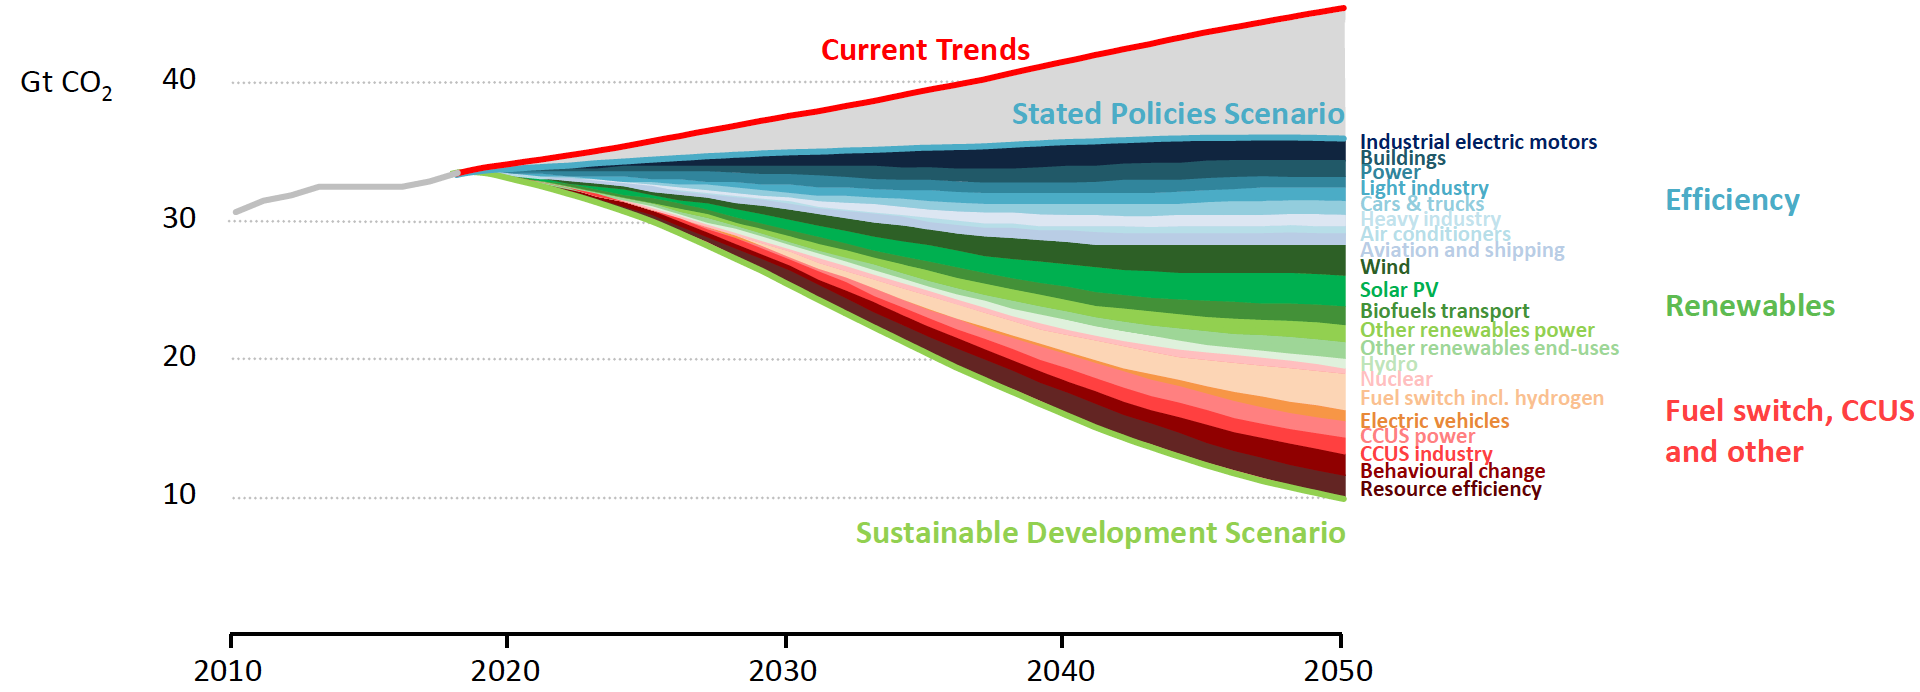
\includegraphics[width=\textwidth]{IEA_WEO_2019.png}
\caption{Energy-related CO2 emissions and reductions by sources in the Sustainable Development Scenario \cite{iea2020world}.}
\label{fig:intro:IEA_WEO_2019}
\end{figure}

In the general perspective to decrease the \gls{GWP} of the primary energy mix, \gls{VRES} like wind and solar, have already emerged as the keystone to defossilise the energy system. However, their intermittency and space disparity could hold back their vaster integration in the future. To address this issue, due to some limitations (\eg range, power, costs) of electricity-focused solutions like \gls{DC} lines, the transport and long-term storage of the renewable electricity produced in excess should be optimised. This challenge can be tackled by \textit{electrofuels} \cite{rozzi2020}. These fuels represent energy carriers where electricity has the major share in the energy balance of the fuel. In practice, this electricity is mainly converted into hydrogen (\ie electrolysis) and then potentially upgraded into more complex fuels (\eg methane, methanol or ammonia). Even if the share of electricity increases in the energy system through the electrification of the end-use demand, gaseous and liquid fuels will keep on being big players during (and after) the energy transition \cite{Ahlgren2012}. They offer three main advantages: infrastructure compatibility, storage and capacity to link sectors (\ie from electricity to mobility, heat, or industry). Development on electrofuels aims at getting them more and more compatible with existing and mature technologies \cite{Ahlgren2012}. An example is carbon-free ammonia-hydrogen blends burned in spark ignition engines \cite{lhuillier2020experimental} or \gls{CHP} applications \cite{pochet202022}. With a growing share of \gls{VRES}, sector coupling is essential to absorb the surplus of electricity from these intermittent production means \cite{robinius2017linking} and integrate them more cost-effectively \cite{brown2018response, limpensECOS2021}. Besides direct electrification of other sectors (\eg electrical heat pumps, \gls{BEV}), \citet{brown2018synergies} showed that converting power to hydrogen and methane was advantageous at high shares of renewables, in their optimisation of the European whole-energy system. Electrofuels have the ability to couple energy and non-energy sectors \cite{Stancin2020}. For instance, electricity produced in excess from \gls{VRES} can be converted into ammonia through the Haber-Bosch process and subsequently transformed into fertiliser - coupling the power and industry sectors \cite{verleysen2020can}. Gas networks present much more storage potential than electrical network (\eg 50 times more in Germany and 300 times more in France) \cite{Rosa2017}. Where batteries exhibit limited storage capacity (up to 10\,MWh) as well as self-discharge losses, electrofuels are an economical solution for high capacity (from 100 GWh) and long-term (\ie from months to years) storage of energy \cite{child2018role, dias2020energy} (see Figure \ref{fig:intro:Storage_electrofuels}). In their analysis of the German transport sector in 2050, \citet{millinger2021electrofuels} highlighted that producing electrofuels can represent a better usage of the ambient \ce{CO2} than \gls{CCS} to supply hydrocarbon fuels while limiting the curtailment of \gls{VRES}. Moreover, some applications (\eg marine, aviation and heavy-duty transport) will be hard to electrify and keep on requiring high-density energy carriers \cite{horvath2018techno, brynolf2018}. These carriers, currently produced from fossil resources, will still consist of hydrocarbons in a renewable world. This is why this thesis rather uses "defossilisation" rather than "decarbonisation" as carbon will still play a key role in a carbon-neutral energy transition \cite{mertens2020carbon}.

\begin{figure}[htbp!]
\centering
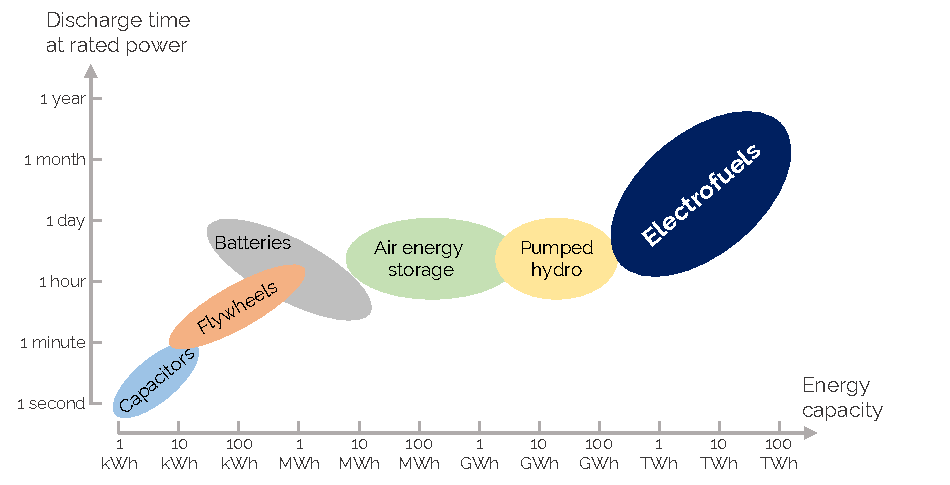
\includegraphics[width=0.9\textwidth]{Storage_electrofuels.pdf}
\caption{Energy carriers and technologies to store electricity. Electrofuels are an economical solution for high capacity and long-term storage of energy. Graph adapted from \cite{ISPT2017}.}
\label{fig:intro:Storage_electrofuels}
\end{figure}

To harvest the maximum potential of synthetic energy carriers in a sustainable transition and maximise the overall system efficiency \cite{mathiesen2015}, it is necessary to study the integration of these fuels within a multi-sector and whole-energy system \cite{Contino2020}. To reach this goal, an energy system optimisation model (ESOM) can optimise the design and the operation of the system to minimise, for instance, its costs or its emissions \cite{zeng2011review}. 

In this research field of energy system planning and scenario analysis, \citet{yue2018review} highlighted that most of ESOMs use a deterministic approach (\ie 75\% out of the 134 reviewed ESOM studies). However, the model structures are inherently uncertain as well as their numerous composing parameters, especially when it comes to define an energy transition strategy for a large-scale system, such as a country. Given the lifetime of the conversion technologies, such strategy implies decisions with long-term impacts (20 to 50 years) where forecasts can be highly unreliable \cite{Moret2017}. Besides the uncertainty on the model structure (not addressed in this work), this long-term and large-system optimisation motivates the need to account for \gls{UQ} and consider it as a major challenge of such models \cite{pfenninger2014energy}. This challenge, along with a large number (\ie more than a hundred) of uncertain parameters and limited information of their distribution, leads to the "curse of dimensionality" \cite{kuo2005lifting}, where the computational burden rapidly explodes with the number of considered uncertain parameters.

On top of dealing with these uncertainties, the reality of decision-makers is a limited foresight into the future \cite{poncelet2016myopic}. In a perfect foresight approach, decision-makers would be able to, from now on, see the ``finish-line of the transition'', \ie 2050 (and beyond), and make the planning decisions once and for all accordingly. On the contrary, they uncover the realisation of these uncertainties step-by-step (\ie in a ``myopic'' way), and progressively act on them to, hopefully, meet the set target to mitigate the climate change. In the objective to respect an overall \ce{CO2}-budget rather than to follow a prescribed \ce{CO2}-emissions trajectory, there was a need for a framework to explore these multiple transition pathways and provide insight about intermediate milestones not to miss. On top of the ``what to do?'', this approach aims at helping the policymakers to answer the  question ``how to do it?''.

Finally, when assessing the robustness of transition pathways provided by \gls{ESOMs}, the literature shows a variety of techniques, \eg Monte-Carlo analysis, stochastic programming or robust optimisation \cite{yue2018review}. However, the robustness is commonly applied to assess the sensibility of the solution regarding the objective function to optimise (\ie the total cost).  Given the complexity of whole-energy system models (\ie multiple sectors and multiple energy carriers) along with the time-scale of the transition and the lot of uncertainties, the total cost does not provide information on the sensibility of the design strategy, \ie the investment decisions. Where \citet{moret2020overcapacity} proposed a method to assess the robustness of a design by investigating the potential overcapacity needed to face uncertainties. However, their work focused on the power sector only and for a target future year, \ie 2035.  The literature was missing an approach to tackle these two challenges: to go beyond the total transition cost encompassing the details of a solution into a single value while assessing the whole-energy system over its whole transition.

\section*{Objectives and tasks}
``\textit{Our task is not to foresee the future, but to enable it.}'' Saint-Exupéry in Citadelle, 1948. In that sense, this thesis aims at providing decision-makers with new methods and informed policies accounting for the intrinsic uncertainties of the future.  Rather than trying, in vain, to answer the question ``What could possibly happen in the future?'', this work rather addresses the ``What could or should we do to make the future possible?''. Given these general context and motivations, the research questions are described as follows:
\begin{itemize}
\item What is the role of electrofuels in the transition pathway of a whole-energy system subject to uncertainties, limited foresight into the future and a \ce{CO2}-budget? What are the key uncertainties driving their import?
\item How to explore the multiple pathway possibilities through the optimisation of a policy, \ie sequence of actions to support a transition?
\item How to assess the robustness of a pathway roadmap defining the design strategy over the transition?
\end{itemize}

To answer these questions, several tasks have been carried out on the whole-energy system model accounting for the uncertainties, the method to explore the myopic pathway of such a system and the approach to assess the robustness of a pathway roadmap.  All this work has been applied to the case of Belgium, a densely populated country with a limited amount of renewable energies, which represents roughly one third of the forecast energy demand \cite{Limpens2020}. This makes it a challenging case to go from a highly fossil-dominated system in 2020 (\ie 73\% of the primary energy mix \cite{spf_economy_2022}) to carbon-neutrality by 2050. 

The model developed and used in the context of this thesis is EnergyScope Pathway \cite{limpens2024pathway}. First introduced by Limpens in his PhD thesis \cite{limpens2021generating}, this model optimises the design and the operation of a whole-energy system over several decades and accounts for the pathway transition from an existing system to a long term target, \ie 2050.  Compared to other models, EnergyScope Pathway introduces a rapid (\ie around 15~min on a personal laptop for the optimisation of a 30-year transition) computational optimisation tool for exploring diverse transition pathways within an entire energy system while maintaining temporal precision (\ie hourly time-resolution) to accurately capture the integration of \gls{VRES}. Based on this model originally implemented in a perfect foresight approach, \ie one overall optimisation for the whole pathway, we have developed the myopic method. In this, the whole time horizon (\ie 30 years) is optimised through a sequence of 10-year long time-windows having a 5-year overlap between each other. To address the question about the role of electrofuels, we have detailed further on their implementation in the model to account for four main ones: hydrogen, methane, ammonia and methanol. Moreover, given their current and (expected) future role into the sector of the \gls{NED}, we have implemented this sector with a similar level of detail as the other sectors of the system, \ie electricity, heat and transport. 

To account for uncertainties, we have used, and adapted to our case study, the work of \citet{Moret2017PhDThesis} and \citet{coppittersthesis} on the uncertainty characterisation and quantification, respecitvely. In his thesis, \citet{Moret2017PhDThesis} developed a framework to obtain uncertainty range for a variety of parameters like cost of purchasing and availability of resources or investment cost and efficiency of technologies. These ranges have then been sampled and propagated through the EnegyScope Pathway via the RHEIA framework developed by \citet{coppittersthesis}. Using the surrogate-modeling approach called \gls{PCE}, this framework allows identifying the uncertain parameters with the biggest impact on the variation of total transition cost or other outputs of interest like the imported amount of electrofuels. 

To explore the different pathway trajectories in this myopic optimisation process, we have applied the \gls{RL} method where an ``agent'' is trained through its interactions with its environment, EnergyScope Pathway, to optimise its policy, \ie sequence of actions to take to support the transition. Starting from the initial state of the energy system in 2020, the agent takes every five years a set of actions until reaching 2050. Although, these actions are taken every five years, they impact the system, for the next ten years - their time window. The intermediate solutions obtained in the middle of the time window are used as a new starting point for the agent that makes a new series of decisions for the next ten years, etc. Repeating the whole transition with different sequences of actions-states allow the agent to come up with an optimised policy towards sustainability, considering the variation of the parameters of its environment.

Finally, in the objective to assess the sensibility to uncertainties of different design transition roadmaps, we have defined an approach to come up with a ``robustness metric''. This approach is based on \gls{PCA} where directions capturing the widest design variations are identified and serve as a frame. Roadmaps resulting from perfect foresight optimisation have been tested in a myopic and uncertain pathways. The results of these myopic runs have then been ``projected'' on the aforementioned frame to be able to compare the robustness of different roadmaps between each other.

\section*{Outline}
This thesis is composed of five chapters to provide answers to the different research questions. Chapter \ref{chap:chap_methodo} brings more details about the different methodological aspects of this work. It starts with the main constraints, parameters and variables of the whole-energy system optimisation model, EnergyScope Pathway. Then, it gives information on the \gls{UQ} approach and the way it has been adapted to the case of Belgium and its transition pathway. Finally, general fundamentals and more case-specific considerations are brought up about the \gls{RL} and \gls{PCA}-based robustness approaches.

Chapter \ref{chap:case_study} presents the case study of this work, \ie Belgium and its energy transition. Without exhaustively detailing the data \cite{limpens2021generating}, this chapter focuses on the main contributions of this work regarding the case study: the \gls{NED}, the implementation of electrofuels and their respective routes of production and consumption, limiting  the cumulative emissions of the transition to a certain \ce{CO2}-budget rather than a prescribed emissions-trajectory and the date related \gls{SMR} as an option to produce nuclear-based electricity in the future.

Chapter \ref{chap:atom_mol} is the first of the three chapters presenting results. In this one, we detail the results of the \gls{GSA} carried out on the Belgian energy transition under the lens of the atom-molecules dilemma. On top of the impact of uncertainties on the total transition cost and the system design in general, we target the impact of having new nuclear capacities by 2040 onward and the driving parameters on the import of electrofuels.

In Chapter \ref{chap:chap_RL}, the rules of the ``\gls{RL} game'' are detailed. In other words, we define the action and state spaces as well as the reward function driving the behaviour of the agent in its quest to optimise its policy. Then, we analyse the results of the learning phase before testing under uncertainties the learned policy versus more ``classic'' myopic optimisation, \ie without the support of such a policy.

After detailing the robustness metric based on the \gls{PCA} approach, Chapter \ref{chap:chap_RobPol} assesses the robustness of different roadmaps resulting of deterministic perfect foresight optimisation under certain conditions: REF, SMR and ROB. The first one, the reference case, considers nominal values for all the uncertain parameters. The SMR case is the one introduced in Chapter \ref{chap:atom_mol} where we allow the model to install \gls{SMR} from 2040 onward. Eventually, the ROB case accounts for the highest values of parameters for those having the biggest impact on the total cost of transition (\ie cost of purchasing energy carriers, industrial \gls{EUD}, interest rate and variable \gls{OPEX} of technologies).

Finally, we draw general conclusions and suggest potential perspectives for future works in terms of uses and further developments of the methodological tools.
%\clearpage

%% -- Chapter 1 - Presentation of EnergyScope TD & Pathway + PCE ---------------------------------
%\chapter{From a whole-energy system model and an uncertainty quantification framework}
%\label{chap:chap_ES_PCE}
%%!TEX root = ../thesis_main.tex
%!TEX encoding = UTF-8 Unicode
In this chapter, we introduce the two main tools, not exhaustively of course (because already presented, in Gauthier and Diederik's theses) on which I based my work: EnergyScope and RHEIA/PCE. I'd like too to talk about the case study (Belgian energy system) that will be addressed all along the manuscript but I'm afraid it'd be too many stuff in one chapter. On the other side, I would not dedicate an entire chapter to any of these three parts. What's your opinion?
\section{EnergyScope: To optimise the energy transition pathway}
\label{sec:energyscope}

\subsection{EnergyScope TD}
\label{subsec:estd}
Presentation of the capacity to model a whole-energy system,with a hourly resolution, and of the main equations of the snapshot model (similarly to what I've done in the electrofuels+UQ paper (\url{https://www.mdpi.com/1996-1073/14/13/4027}).

\subsection{EnergyScope Pathway}
\label{subsec:espathway}
From snapshot to pathway optimisation, presentation of the main equations to link the representative years, focus on the salvage value (not presented in Gauthier's thesis but well in our Pathway paper)

\section{RHEIA: To quantify the uncertainties}
\label{sec:rheia}


\subsection{Uncertainty characterisation}
\label{subsec:uncert_charac}
Presentation here of the uncertainty characterisation from S. Moret and adding some parameters specific to the pathway model (\eg $\Delta_{\text{change}}$ linked to change speed) or specific to the main case study (\eg possibility to have nuclear SMR from 2040)


\subsection{Polynomial Chaos Expansion}
\label{subsec:pce}
Similarly to what we did in the electrofuels+UQ paper (\url{https://www.mdpi.com/1996-1073/14/13/4027}), presentation of the PCE and Sobol' sequence (which is a more optimised way to explore the ranges of uncertainties, compared, for instance, to random exploration).


\subsection{Preliminary screening and selection}
\label{subsec:screening}
Similarly to what we did in the electrofuels+UQ paper (\url{https://www.mdpi.com/1996-1073/14/13/4027}), emphasise that we only consider a limited amount of uncertain parameters to keep a reasonable computation time while capturing the impact of (almost) all the uncertainties.

\section{Case study: The Belgian energy system}
\label{sec:case_study}
Similarly to what we did in the electrofuels+UQ paper (\url{https://www.mdpi.com/1996-1073/14/13/4027}),I'd present generally here the case study, much shorter than what Gauthier did in his thesis. It'd be presenting the different sets of resources, technologies and demands.

Here, I could integrate the information on the NED and how important it is to consider it as it represents 10\% worldwide (and even 20\% in Belgium) of the energy consumption, especially because it is usually a sector that is overlooked in whole-energy system optimisation.










%\clearpage


%% -- Chapter 2 - UQ on a snapshot model, assessment of electrofuels ---------------------------------
%\chapter{Electrofuels and uncertainties in a target future year}
%\label{chap:chap_electro_uq}
%%!TEX root = ../thesis_main.tex
%!TEX encoding = UTF-8 Unicode

In this chapter aims at showing the first step of uncertainty quantification and highlight a first insight in terms of impacting parameters. It'd also highlight that depending on the gwp\_limit 
\section{From a cost-optimised to a carbon-neutral Belgian energy system: progressive defossilisation}
\label{sec:chap_2_ses_sec2}
In this section, I'd include the section 2 of the electrofuels+UQ paper (\url{https://www.mdpi.com/1996-1073/14/13/4027})(without 2.2 where I presented EnergyScope that I'd include in Chapter 1).

\subsection{Electrofuels}
\label{subsec:chap2_electrofuels}
This section would be as the section 2.1 of the electrofuels+UQ paper (\url{https://www.mdpi.com/1996-1073/14/13/4027}), where I present more specficially how electrofuels are implemented in the model

\subsection{Reference Case Study: The Belgian Energy System in 2050}
\label{subsec:chap2_case_study}
Basically section 2.3 of the electrofuels+UQ paper (\url{https://www.mdpi.com/1996-1073/14/13/4027}), where I present more specficially how electrofuels are implemented in the model where I present what a cost-optimised (without gwp-constraint) Belgian energy system would look like

\subsection{A step by step defossilisation of the snapshot system}
\label{subsec:chap2_defossilisation}
As in section 2.4, quickly show how we implement the defossilisation without having an entire pathway.

\section{Results}
\label{sec:chap2_results}
Similar to Section 4 of the electrofuels+UQ paper (\url{https://www.mdpi.com/1996-1073/14/13/4027}). There'll be work to generate up-to-date results as the model evolved (no more FC\_cars but BEV, for instance)
\subsection{Statistical analysis of the cost}
\label{subsec:chap_2_stat_analysis}

\subsection{Critical parameters}
\label{subsec:chap_2_crit_param}

\section{Discussion and perspective with the literature}
Similar to section 5.1 of the electrofuels+UQ paper (\url{https://www.mdpi.com/1996-1073/14/13/4027})

%\clearpage

%% -- Chapter 3 - Case study -----------------------------
\clearemptydoublepage
\chapter{Case study: the Belgian energy system} 
\label{chap:case_study}
%\begin{flushright}
%%%\emph{``For the things we have to learn before we can do them, we learn by doing them.''}\\%Each wrong scenario you have analysed, is a wrong decision you won't made.''}\\
%%%Aristote
%\emph{All models are wrong, but some are useful.}\\
%George P. Box
%\end{flushright}

%\medskip
%
%\begin{mybox}{Chapter overview}
%\begin{itemize}[left=0em]%[leftmargin=0cm,itemindent=.5cm,labelwidth=\itemindent,labelsep=0cm,align=left]
%\setlength\itemsep{-0.3em}
%\item Belgian energy system overview%Case studies: the Belgian energy systems during the transition (2015-2050).
%\end{itemize}
%\vspace{-0.3cm}
%
%\emph{This chapter is an improved and extended case study version of \citet{Limpens_belgian_2020}}.
%\end{mybox}
%
%\medskip

As detailed by \citet{limpens2024pathway}, the analysis carried out in this work can be applied to any regional whole-energy system. As a densely-populated and highly-industrialised country with limited local renewable potentials (\ie mainly solar and wind representing up to 50\% of the primary mix by 2050), the transition of Belgium from a fossil-dominated system in 2020 (Appendix \ref{app:bel_2020}) to carbon-neutrality in 2050 makes it an intricate case study. Moreover, this case study and the subsequent analyses can be transferred - to some extent - to other industrialised countries highly dependent on fossil fuels with limited local renewable potentials (\eg the Netherlands or Germany) \cite{dommisse2020modelling}. This chapter presents the different demands to satisfy, with a particular focus on the non-energy demand, as well as the resources available and the conversion technologies to supply those. For a comprehensive understanding and detailed descriptions of the technologies, please refer to the documentation \cite{readthedocs_pathway}. Then, the uncertainty ranges considered for some of the parameters are detailed. Finally, the \ce{CO2}-budget over the 2020-2050 transition is presented.

\section*{Contributions}
\label{sec:cs:contributions}
First, as pointed out by \citet{rixhon2022integration}, where most of the studies assessing whole-energy system integrate energy demands (\ie electricity, heart and mobility), the \acrfull{NED} is often not considered. The latter is defined as ‘\textit{energy products used as raw materials in the different sectors; that is not consumed as a fuel or transformed into another fuel}’ \cite{Eurostat2019}. The previous analyses carried out with \gls{ESTD} considered the non-energy demand as the related primary energy needs, \ie either natural gas or \gls{LFO}. To minimise the total cost of the system, the model simply selected the cheapest between the two resources (\ie natural gas). This work goes one step further and accounts for the \gls{NED} as a demand of three commodities (\ie \gls{HVC}, ammonia and methanol) as well as with associated production technologies. This allows bringing the non-energy sector to a similar level of details as the other sectors.  Keeping the same methodology to define \gls{EUD} in EnergyScope as \citet{Limpens2020}, this work considers updated values given the latest release of the \og EU reference scenario 2020 : energy, transport and GHG emissions: Trends to 2050 \fg by the European Commission \cite{EuropeanCommission2021}.

Second, given the focus of this work on the electrofuels, the case study includes a more explicit representation of them: where the previous definition of the case study considered only renewable hydrogen and methane \cite{limpens2021generating}, now, e-ammonia and e-methanol (as well as their fossil-based equivalents), are implemented in the case study. As detailed later on, these electrofuels are considered as renewable in the sense that their \gls{GWP} is zero. This more explicit representation of the molecules themselves also comes with a more exhaustive integration of the ways to produce and use them in the system. For instance, considering the case of ammonia, on the top of the import routes, the Haber-Bosch process ,on one hand, is accounted for to supply this molecule. On the other hand, ammonia-driven \gls{CCGT} or ammonia-cracking-to-hydrogen are included as ways to consume it.

Third, as nuclear energy could be a real game-changer in the energy transition worldwide \cite{IEA2022nuclear}, and especially in Belgium, this thesis has integrated the uncertain potential to install \gls{SMR} from 2040 onward.

Fourth, where previous works considered a prescribed \ce{CO2} trajectory to reach carbon-neutrality by 2050 \cite{limpens2021generating, limpens2024pathway}, the case study analysed in this thesis is subject to a \ce{CO2}-budget for the transition, \ie limiting the total amount of emissions over the transition. Based on the estimated world budget provided by the \gls{IPCC} to limit the global warming to +1.5°C by the end of the century, the grandfathering approach has been used to allocate part of this budget to the Belgian energy transition.

Finally, to a smaller extent, this work includes updated values for some parameters compared to the work of \citet{limpens2021generating}. The main change concerns the cost and performance of private mobility vehicles, which is specifically a key components in the European \cite{biresselioglu2018electric} and Belgian \cite{BFP_mob} energy transitions. Based on the work of \citet{national2013transitions}, \citet{limpens2021generating} excessively favoured \gls{FC} car versus \gls{BEV}. Besides their lower efficiencies (\ie about 50\% less efficient), \gls{FC} car had the lion share of the private mobility, compared to \gls{BEV} given the higher CAPEX (\ie up to 10\% more expensive) and limited range (\ie 24kWh battery) of the latter, in previous works \gls{limpens2021generating,rixhon2021role}. In these, the more limited potential to import electricity from abroad and produce it locally via \gls{VRES} forced the model to rather electrify the low-temperature heat sector rather than the private mobility running on supposedly infinitely available renewable hydrogen. To align with other similar works on the modelling of whole-energy system \cite{schnidrig2021modelling, EuropeanCommission2021}, the CAPEX and efficiency of fuel cell cars have been increased. Regarding \gls{BEV}, while the CAPEX has been kept unchanged, the efficiency and the battery capacity, \ie the range, have been increased. As seen in the results, this change of data made \gls{BEV} often more competitive than its hydrogen-based equivalent. 

\section{End-use demands}
\label{sec:cs:demand}
End-use demands, exogenously imposed as inputs to the model, are characterised by yearly quantities to satisfy and are also distributed over the different hours of each representative years of the transition, in order to account for their daily or seasonal variability \cite{Limpens2020,limpens2021generating}. In this work, the yearly end-use demands (EUD) for all sectors are calculated from the forecast proposed by the European Commission for Belgium (Appendix 2 in report \cite{EuropeanCommission2021}). 

\subsection{Non-energy demand}
\label{subsec:cs:NED}
The \gls{NED} currently represents around 20\% of the final energy consumption in Belgium \cite{FPSEconomy2021}.  This section summarises the rationale of adding a higher level of details to the\gls{NED} compared to what was done in the previous version of the case study \cite{limpens2021generating}. Then, it explains the methodology used to quantify this demand.\\

\myparagraph{Definition and historical trend}\\

\noindent
The \gls{NED} can be split into four main categories of final molecules \cite{IEA2018_petrochemicals}: (i) \gls{HVC} (worldwide production of $\sim$365Mt/year, equivalent to $\sim$4770TWh/year); (ii) ammonia ($\sim$185Mt/year, equivalent to $\sim$964TWh/year); (iii) methanol ($\sim$100Mt/year, equivalent to $\sim$540TWh/year) and (iv) the other products. \Gls{HVC} gather the light olefins (e.g. ethylene, propylene) and aromatics (benzene, toluene, xylene – BTX), mainly for the production of plastics, synthetic fibers or rubber. Their production today relies mainly on petroleum products such as naphtha, ethane or liquified petroleum gas. Ammonia is  mainly used for the production of fertilizers ($\sim$80\% of global ammonia consumption). Its production is dominated by fossil gas via steam methane reforming to produce hydrogen, used as feedstock in the Haber-Bosch process. Methanol is mainly converted to formaldehyde (resin) but also used for the production of other chemicals (e.g. solvents and gasoline-blends). Currently, its synthesis, like ammonia, is mainly relying on natural gas via steam methane reforming. Finally, the other products gather all chemicals not mentioned in the other categories such as bitumen, lubricants and other heavy products from oil refineries \cite{daioglou2014energy}.\\

Over the recent history, there has been a relatively constant evolution of three main categories of the final consumption for non-energy use in Belgium, \cite{statbel_NED_2019}: (i) naphtha and \gls{LPG} (between 59\% and 67\% of the total final consumption, around 59.4\,TWh in 2019), (ii) fossil gas (between 9\% and 14\%, 11.8\,TWh in 2019), and (iii) others (\ie bitumen, coal tar and other oil products) (between 21\% and 28\%). Naphtha and \gls{LPG} are consumed in a naphtha cracker, which results in ethylene and propylene, what will be considered as \gls{HVC} in the rest of this work. Similarly, fossil gas, as non-energy carrier, is used in steam methane reformer to produce the required hydrogen to the synthesis process of ammonia. The small shares of bitumen and coal tar are respectively used for roadworks and to produce synthetic gas through gasification. Finally \og other oil products'' take into account, indistinguishably, tar and sulphur as well as by-products of the refineries (\eg \gls{BTX}). About methanol, there is currently no production plant in Belgium even if the country plays a role in trading this commodity between its neighbouring countries and consumes part of what it imports.\\

\myparagraph{Methodology of quantification}\\

\noindent
The non-energy demand studied in this analysis focuses on the chemical industry (more than 90\% of the non-energy use in Belgium) and, similarly to other studies \cite{IEA2018_petrochemicals, daioglou2014energy}, is split between the three aforementioned main groups of products (\ie \gls{HVC}, ammonia and methanol). Before describing these three demands, this study excludes bitumen, coal tar and \og other oil products\fg. The first two represent marginal shares of the current non-energy use (\ie 4\% and 5\% respectively) in such a way that they should not affect the conclusions provided by this study. As described previously, the latest are mostly by-products from refineries that the system uses because they are available. However, in a perspective of defossilisation, since the future of fossil-based refineries is unclear, they have not been implemented in this study nor their by-products.\\

Regarding \gls{HVC}, the future of their production is highly uncertain. Because of the new regulations and strategies promoting recycling and limitation of single-use plastics \cite{EU_plastics}.  Besides this uncertainty, Belgium stays a major exporter as approximately 2/3 of plastic raw materials produced locally are exported abroad \cite{agoria_plastics}. Even if a significant part of \gls{HVC} produced in Belgium is not locally consumed, this demand has been set based on the assumption that Belgium will keep its industrial activity in this sector. In other words, this assumption does not deduce the part of local production  of \gls{HVC} being then exported (and not consumed locally), unlike ammonia and methanol, which will be more traded commodities in the future (as energy carriers and non-energy products). Therefore, the actual demand of \gls{HVC} is inferred from the consumption of naphtha and \gls{LPG} as non-energy use as well as energy-carrier in the chemical and petrochemical industries \cite{statbel_NED_2019}. This assumption is based on the fact that, in the conversion processes to produce \gls{HVC} from naphtha or \gls{LPG}, these fuels also serve as energy-carrier to supply the process itself. Then, given the respective efficiencies (1.83t$_{\text{naphtha}}$/t$_{\text{HVC}}$ and 1.67t$_{\text{LPG}}$/t$_{\text{HVC}}$) \cite{IEA2018_petrochemicals}, the current demand of \gls{HVC} is estimated equal to 3069\,kt, without making distinctions between the different chemicals (\ie ethylene, propylene and \gls{BTX}). \\

The ammonia sector in Belgium is quite different: the country locally produces and imports ammonia much more than it exports it. Thanks to a database from the United Nations \cite{UN_statistics} and the National Bank of Belgium, it has been identified that, over the last ten years, Belgium has imported 1010\,kt of ammonia, exported 105\,kt and locally produced 990\,kt on average. Therefore, on top of the local production, the net import (\ie import minus export) is also included in this non-energy demand. This gives a current demand of 1895\,kt of ammonia.\\

Concerning the demand of methanol, similarly to ammonia, this work solely considers the net imports as there is no local production in Belgium. To define the actual non-energy demand of methanol, only a 51\%-share of this net import is kept since, according to the Methanol Institute and \gls{MMSA}, this share is used for formaldehyde production in Belgium \cite{MMSA51}. Currently, the rest of the methanol is used for energy purposes, mostly as \gls{MTBE} in gasoline blending. This methodology gives a current non-energy demand of methanol of 269\,kt.\\

Eventually, after converting these masses of products into energy content (\ie LHV: \gls{HVC} - 47\,MJ/kg, ammonia - 18.8\,MJ/kg and methanol - 19.9\,MJ/kg), two final assumptions are made: (i) the current shares of each of the three commodities (\ie 77.9\%, 19.2\% and 2.9\% for \gls{HVC}, ammonia and methanol, respectively) are supposed to remain unchanged over the transition; (ii) the overall \gls{NED}, in absolute terms, follows the growing rate presented by \citet{EuropeanCommission2016}, \ie around 7\% between 2020 and 2050.

\subsection{Forecast of the demands over the transition}
\label{subsec:cs:EUD_forecast}
In their latest report \cite{EuropeanCommission2021}, the European Commission forecasts a significant and abrupt increase of the \gls{NED} compared to their previous report \cite{EuropeanCommission2016}, \ie +80\% over the 2020-2030 time window. Given this discrepancy that is unsubstantiated and specific to the case of Belgium, the evolution trend of the \gls{NED} of the current work has been inferred from the previous edition, published in 2016, \cite{EuropeanCommission2016}. Between 2020 and 2050, one observes a noteworthy increase of the electricity (+40\%), passenger (+45\%) and freight mobility (+35\%) demands (see \Cref{fig:cs_demands}). The rise of the non-energy demand is more limited, \ie +6\%, whereas the heating demands is forecast to decrease: -11\% for the low-temperature heat demand and -3\% for the high-temperature heat demand. This is explained by a better insulation of buildings and an improved efficiency of industrial processes. Regarding the center graph of \Cref{fig:cs_demands}, it is the aggregation of the same data as in the left graph but per category, rather than per sector, with the non-energy demand being associated with the industry. This illustrates how industrialised is Belgium, compared to households and services, and, consequently, highly energy-intensive. The right graph of \Cref{fig:cs_demands} gives the passenger and the freight mobility. The sharp increase from 2020 to 2025 is due the COVID-crisis that has significantly reduced these demands in 2020. As far as the hourly discretisation of these demands is concerned, time series are based on historical values of 2015 for the fluctuating parts of electricity and low-temperature heating demands \cite{Limpens2020}. A daily time series is used for the passenger mobility and applied similarly to every typical days. Finally, for the other demands (\ie high-temperature heat, freight mobility, \gls{NED} and constant share of electricity and low-temperature heat demands), the yearly demand is distributed uniformly over the different hours of the year.

\begin{figure}[htbp!]
\centering
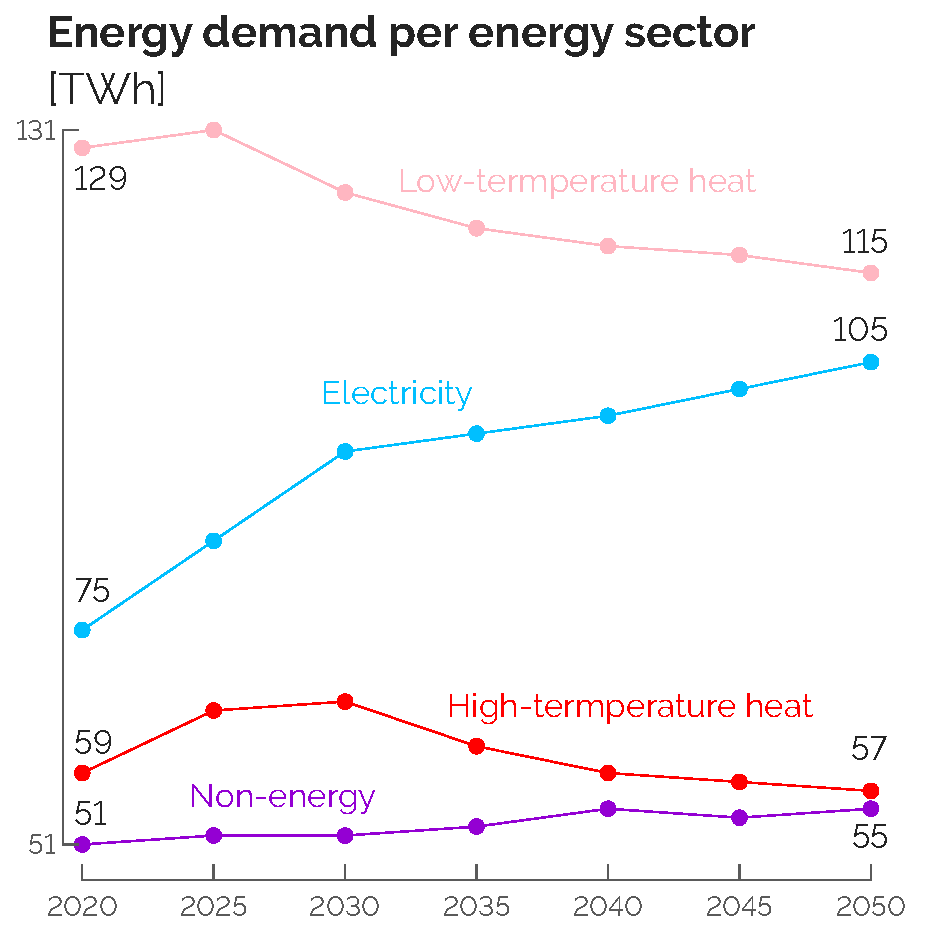
\includegraphics[width=0.49\textwidth]{EUD_sec.pdf}
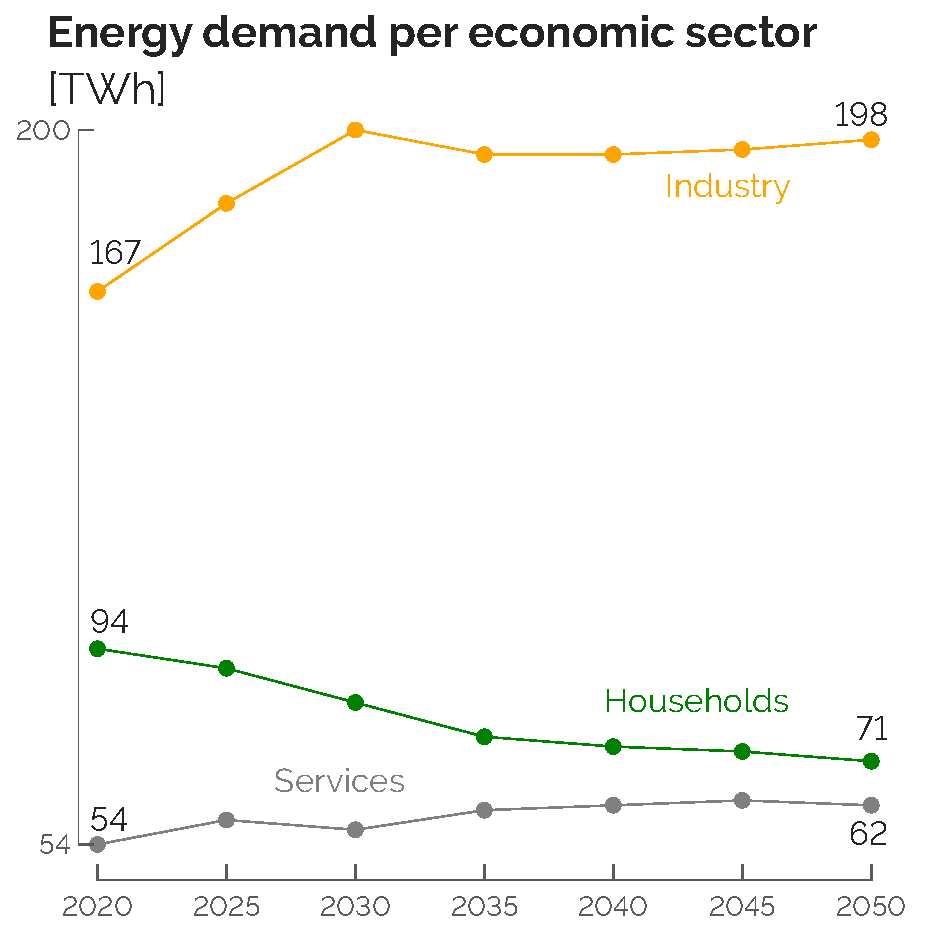
\includegraphics[width=0.49\textwidth]{EUD_cat.pdf}
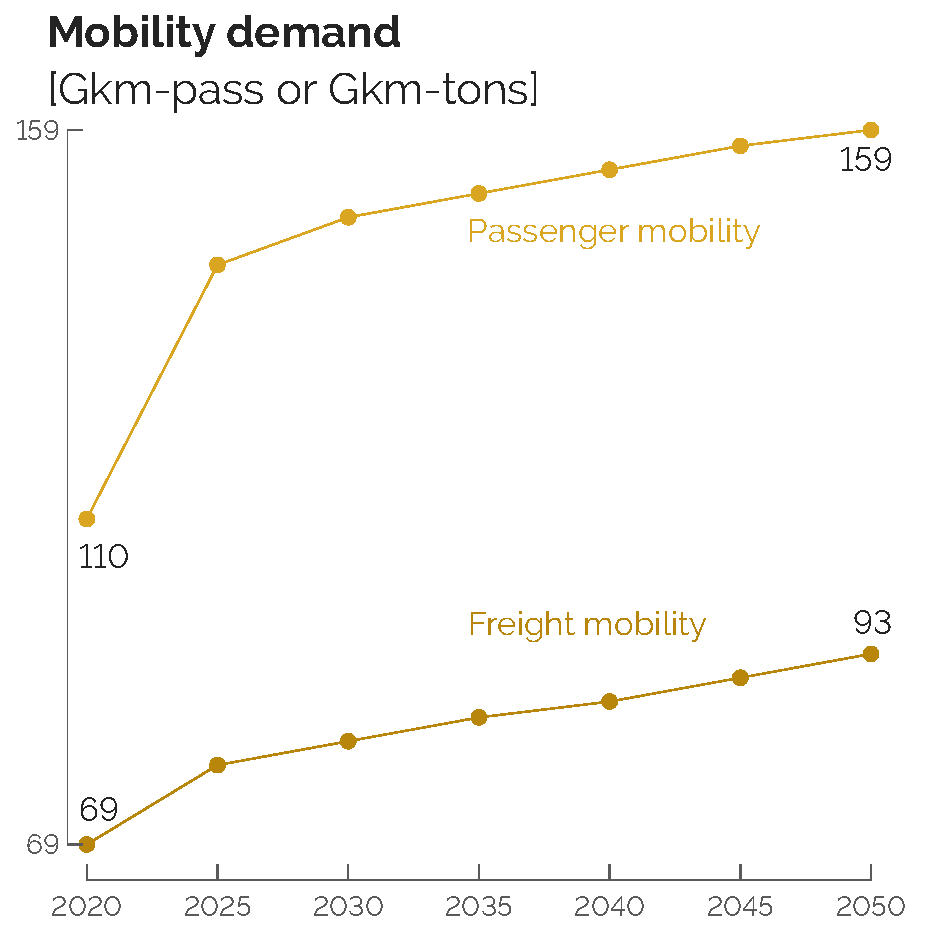
\includegraphics[width=0.49\textwidth]{EUD_mob.pdf}
\caption{EnergyScope splits the whole-energy system end-use demands (EUD) into two sets: (non)-energy and transport-related. This figure presents the nominal values of each of these demands. In the center graph, the non-energy demand has been fully associated with the industrial demand. As detailed previously, the non-energy demand is expressed in tons of physical products (\ie \glsxtrfull{HVC}, ammonia and methanol) and then translated into their respective energy equivalent, in TWh.}
\label{fig:cs_demands}
\end{figure}


\section{Resources}
\label{sec:cs:resources}
To supply the aforementioned demands, EnergyScope Pathway implements a variety of resources defined by their cost of purchasing, $\mathit{c}_{\mathrm{op}}$, their global warming potential, $\mathit{gwp}_{\mathrm{op}}$, as well as their 
availability, as detailed by \citet{limpens2024pathway}. First, the evolution of the respective costs of purchasing is presented (see \Cref{fig:cs_resources_cost}). Regarding ``renewable electrofuels'', these are in line with the recent study of \citet{genge2023supply} who carried out an extensive review and ``meta-analysis\cite{grant2009typology,page2021prisma} of 30 studies on the supply costs of chemical energy carriers''. Then, besides their cost, the resources are either limited or unlimited in terms of availability and either renewable or not. The limitation in terms of availability can be direct or indirect. On the one hand, woody (23.4\,TWh) and wet biomass (38.9\,TWh) are arbitrarily limited by their local potentials and the consumption of waste (17.8\,TWh) and coal (33.4\,TWh) is assumed not to exceed the current use. On the other hand, wind, solar, hydro and uranium are limited by the technical potentials of \gls{PV} panels (59.2\,GW), onshore (10\,GW) and offshore (6\,GW) wind turbines, run-of-the-river power plants (0.1\,GW) and nuclear power plants (6\,GW), respectively. In line with the work of \citet{PATHS2050} and the maximum capacity of conventional nuclear reactors that have been installed in Belgium, the same 6\,GW are assumed to be the maximum capacity for \gls{SMR}. Imported electricity is limited in two ways: the potential of instantaneous capacity of interconnection with neighbouring countries (\ie 11.9\,GW by 2050 \cite{ELIA_2050}) and a limitation to 30\% of the yearly electricity end-use demand (\ie 32.4\,TWh by 2050) \cite{limpens2021generating}. In the current work, the electrofuels (\ie e-methane, e-hydrogen, e-methanol and e-ammonia) are assumed to be ``sustainable" in the sense that they do not increase the concentration of \ce{CO2} in the atmosphere \cite{rixhon2021terminology}. In practice, it means that their \gls{GWP} is assumed to be zero in the model. Regarding specifically these electrofuels, the \citet{h2coalition} has carried out an extensive techno-economic analysis to estimate their respective cost of purchasing, after having identified some key locations from which importing these energy carriers (\eg Chile, Australia or Morocco). As the amount to import from each of these locations is hard to forecast, the current work considers the average cost between the different locations. Besides these, every other resource has its specific \gls{GWP} like coal ($\mathit{gwp}_{\mathrm{op,coal}}=0.40$\,kt$_{\ce{CO2},\text{eq}}$/GWh), natural gas ($\mathit{gwp}_{\mathrm{op,NG}}=0.27$\,kt$_{\ce{CO2},\text{eq}}$/GWh) or the fossil-based molecules equivalent to the electrofuels (\eg $\mathit{gwp}_{\mathrm{op,ammonia}}=0.46$\,kt$_{\ce{CO2},\text{eq}}$/GWh or $\mathit{gwp}_{\mathrm{op,methanol}}=0.41$\,kt$_{\ce{CO2},\text{eq}}$/GWh).

\begin{figure}[htbp!]
\centering

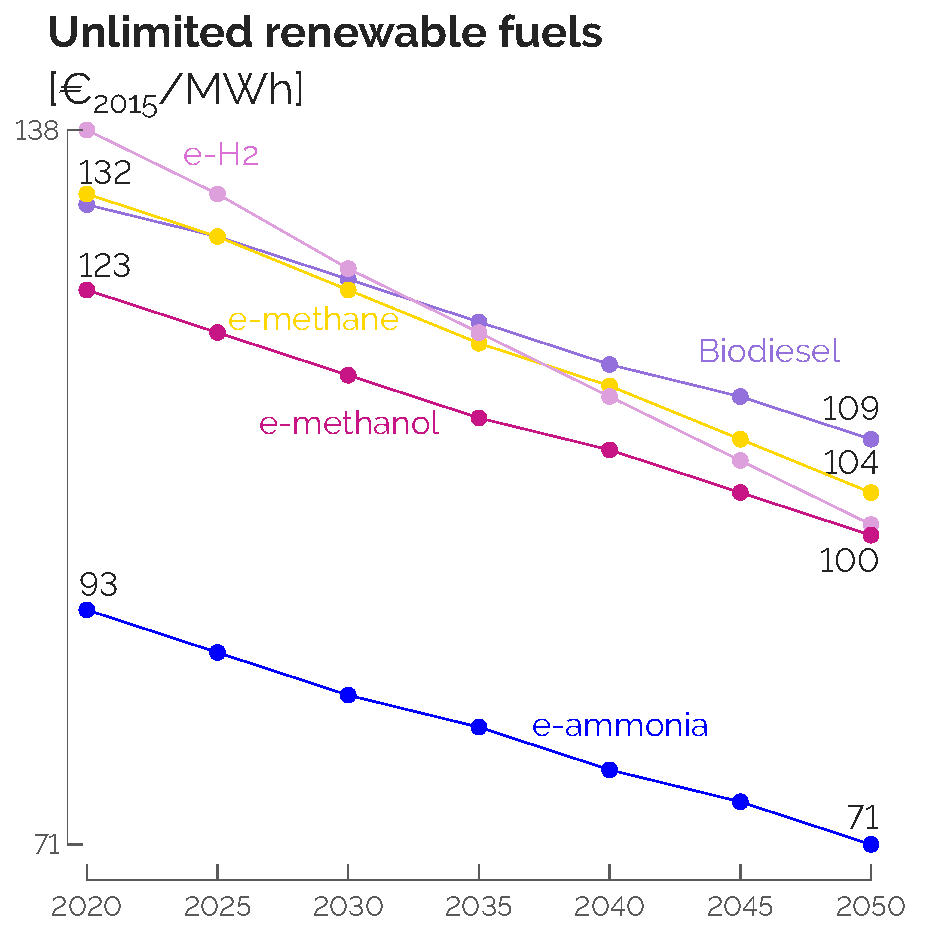
\includegraphics[width=0.49\textwidth]{Res_ren.pdf}
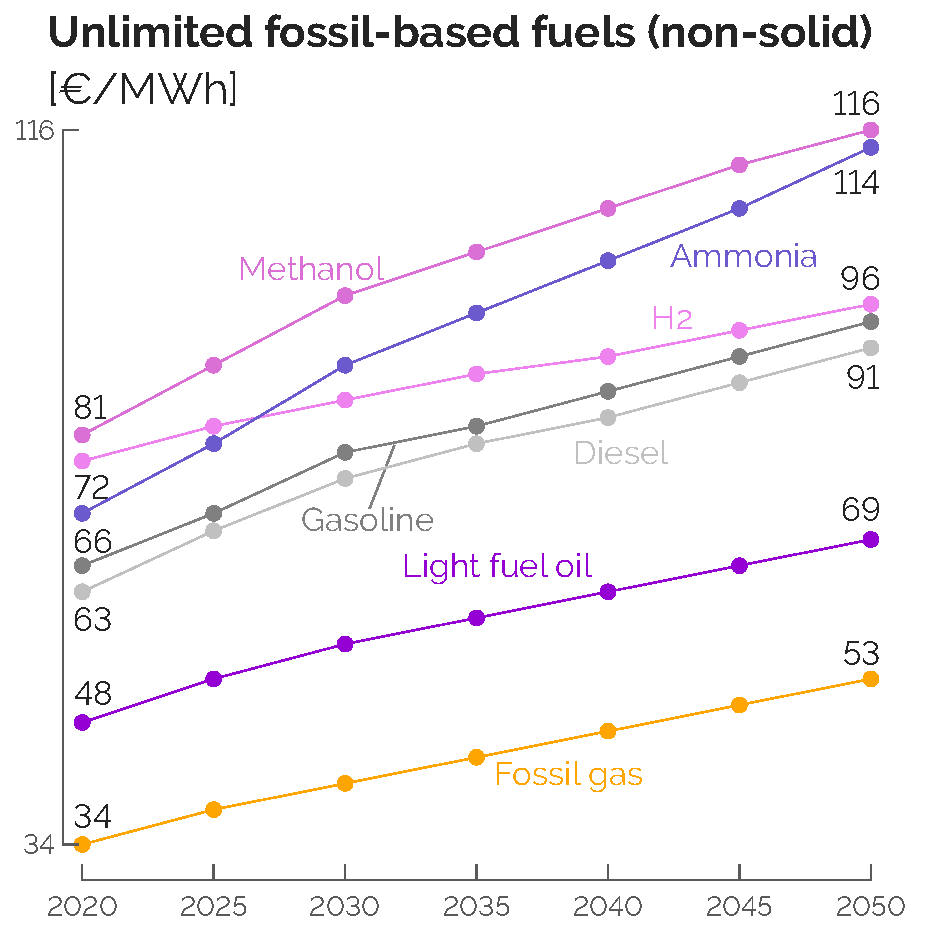
\includegraphics[width=0.49\textwidth]{Res_foss.pdf}
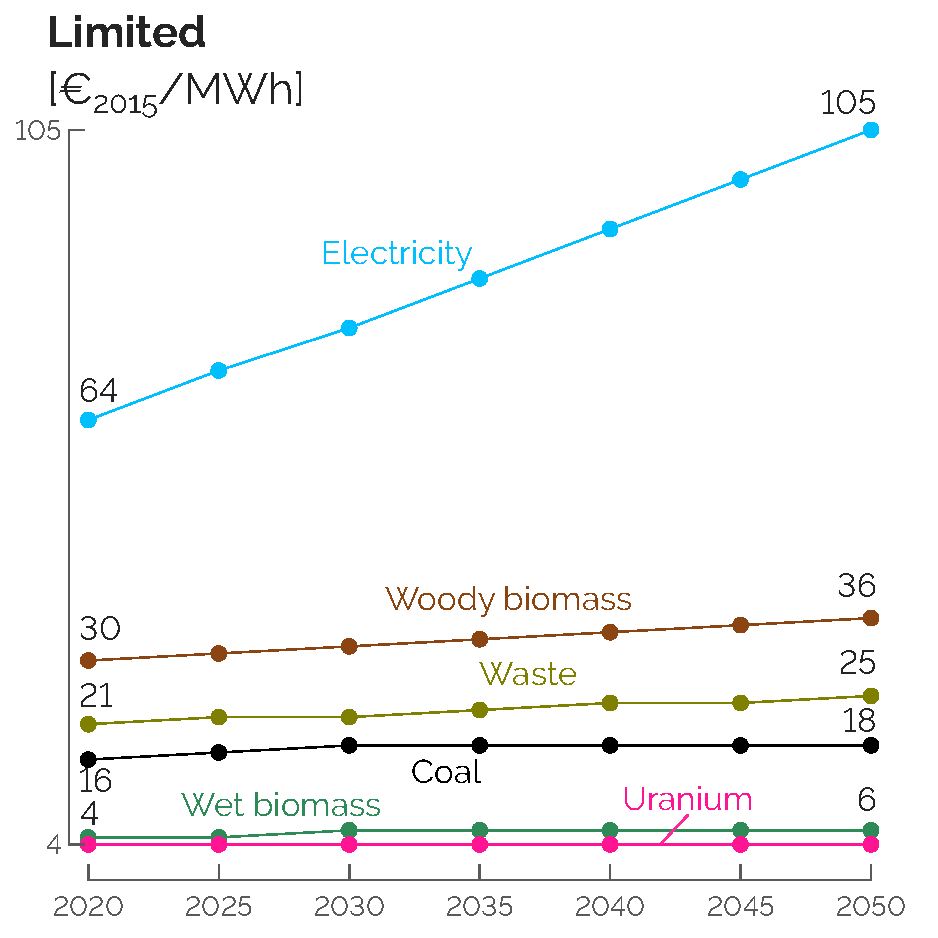
\includegraphics[width=0.49\textwidth]{Res_others.pdf}
\caption{Cost of purchasing the different resources. Besides the free local renewables (\ie sun, wind and hydro) limited by technical potentials, EnergyScope accounts for renewable energy carriers and their respective fossil counterparts (left and center graphs). These fuels can be imported from abroad without limitation on their availability. Other carriers are limited either by their local potentials (\ie biomass and waste) or other considerations like the power grid interconnections or the capacity of nuclear power plants.}
\label{fig:cs_resources_cost}
\end{figure}


\section{Conversion technologies}
\label{sec:cs:technologies}
As the end-use demands are defined as energy (and non-energy with the \gls{NED}) services rather than a certain quantity of oil or solar irradiance, for instance, technologies are implemented to convert these resources into the end-use demands. Besides their CAPEX, OPEX and lifetime defined in Section \ref{sec:meth:ES}, production and conversion technologies (\ie \gls{CCGT}, car or boiler) have a conversion efficiency whereas storage technologies (\ie thermal storage, battery or molecule storage) exhibit their own charge/discharge losses. There are also infrastructure technologies. They encompass, for instance, the power grid, the \gls{DHN} or technologies to produce intermediate energy carriers (\eg wood pyrolysis, biomethanolation or steam methane reforming to produce hydrogen). Not digging into too much details about the exhaustive list of these technologies presented in previous works \cite{limpens2021generating}, this section rather focuses on the implementation of \glsxtrfull{SMR} then the technologies to supply the \glsxtrfull{NED}.\\

\subsection{Small modular reactor}
\label{subsec:cs:SMR_tech}

A specific attention is to put on the implementation of \gls{SMR} whereas the 6\,GW of conventional nuclear are assumed to drop to 2\,GW in 2025 and total phase-out by 2035. Similarly to the analysis of \citet{PATHS2050}, a Belgian consortium for energy research, and in line with the Belgian Nuclear Research Centre (SCK-CEN) \cite{SCK-CEN_SMR}, \gls{SMR} are implemented with the features listed in \Cref{tab:SMR_features}. Where most of the features are similar to conventional nuclear power plants, it differs from these on two main points: their potential year start, 2040, and their flexibility. Indeed, unlike the current nuclear power plants, constrained in the model to produce a constant power output at every hour of the year (\ie baseload production as it is actually the case in Belgium), SMRs, are flexible in the sense that their production can vary between 0 and their full capacity independently at any hour of each representative year. Here, we simplify SMRs as only producing electricity and disregard the heat produced by the nuclear reaction. This is considered as lost to the atmosphere.

\begin{table}[htbp!]
\caption{Nominal features of the SMRs in EnergyScope. \gls{SMR} exhibits the advantage to have a fully flexible production (\ie between 0 to the full capacity) unlike conventional nuclear that is constrained to produce a constant baseload at every hour of the year.}
\label{tab:SMR_features}
\begin{minipage}{\linewidth}
\centering
\begin{tabular}{l c c}
\toprule
\textbf{Feature} & \textbf{Value} & \textbf{Unit}\\
\midrule
CAPEX & 4850 & €/kW \\
Annual OPEX & 103 & €/kW/year \\
Lifetime & 60 & year \\
Efficiency & 40\% & -\\
Maximum capacity & 6 & GW \\
Annual availability & 85\%\footnote{\label{foot:avail_SMR}This annual availability accounts for yearly maintenance where the reactors might not operate or, at least, not at their maximum capacity. } & -\\
Operational year & 2040\footnote{\label{foot:op_year_SMR}2040 is the soonest year at which \gls{SMR} could be available, optimistically assuming industrial prototypes being completed by 2035 and 5 additional years for their commercial installation.} & - \\
Flexibility & Full & - \\
\bottomrule							

\end{tabular}
\end{minipage}
\end{table}


%\begin{table}[htbp!]
%\caption{Nominal features of the SMRs in EnergyScope. \gls{SMR} exhibits the advantage to have a fully flexible production (\ie between 0 to the full capacity) unlike conventional nuclear that is constrained to produce a constant baseload at every hour of the year.}
%\label{tab:SMR_features}
%\centering
%\begin{tabular}{l c c|c}
%\toprule
%\multirow{2}{*}{\textbf{Feature}} & \multirow{2}{*}{\textbf{Value}} & \multirow{2}{*}{\textbf{Unit}} & \textbf{Similarity with}\\
% & & & \textbf{conventional nuclear}\\
%\midrule
%CAPEX & 4850 & €/kW & \checkmark\\
%Annual OPEX & 103 & €/kW/year & \checkmark\\
%Lifetime & 60 & year & \checkmark\\
%Efficiency & 40\% & -& \checkmark\\
%Maximum capacity & 6 & GW & \checkmark\\
%Annual availability & 85\%\footnote{\label{foot:avail_SMR}This annual availability accounts for yearly maintenance where the reactors might not operate or, at least, not at their maximum capacity. } & -& \checkmark\\
%\midrule
%Operational year & 2040\footnote{\label{foot:op_year_SMR}2040 is the soonest year at which \gls{SMR} could be available, optimistically assuming industrial prototypes being completed by 2035 and 5 additional years for their commercial installation.} & - & \xmark\\
%Flexibility & Full & - & \xmark\\
%\bottomrule							
%
%\end{tabular}
%\end{table}

For the sake of comparison, the \gls{LCOE} of the principal technologies to produce electricity, based on the computation used by \citet{limpens2021generating}, are detailed (see \Cref{fig:LCOE}). Not including here the cost of integrating a technology in the system (\eg reinforcement of the grid and storage capacities for \gls{VRES}), the \gls{LCOE} aims at aggregating and normalizing the CAPEX and OPEX of technologies providing a common commodity, \ie electricity. Compared to the other flexible generation units (\ie \gls{CCGT}), \gls{SMR} is significantly more cost-effective. Besides being about six times more capital-intensive in €/kW, the investment is amortized over a longer expected lifetime (\ie 60 years versus 25 for \gls{CCGT}). Moreover, the cost of purchasing uranium driving \gls{SMR} is expected to remain stable and low whereas the expected increase of the cost of purchasing fossil fuels dominates the \gls{LCOE} of \gls{CCGT}. In addition, one sees that \gls{CCGT} supplied by e-ammonia outcompetes its e-methane equivalent, unlike their respective fossil-based equivalent. This due to the fact that e-ammonia, not requiring carbon capture, is expected to be more cost-effective to produce versus e-methane \cite{h2coalition}. On the contrary, fossil-based ammonia, mostly relying on steam methane reforming, requires additional steps in the production process compared to fossil gas, as introduced in Section \ref{subsec:cs:NED}.

\begin{figure}[htbp!]
\centering
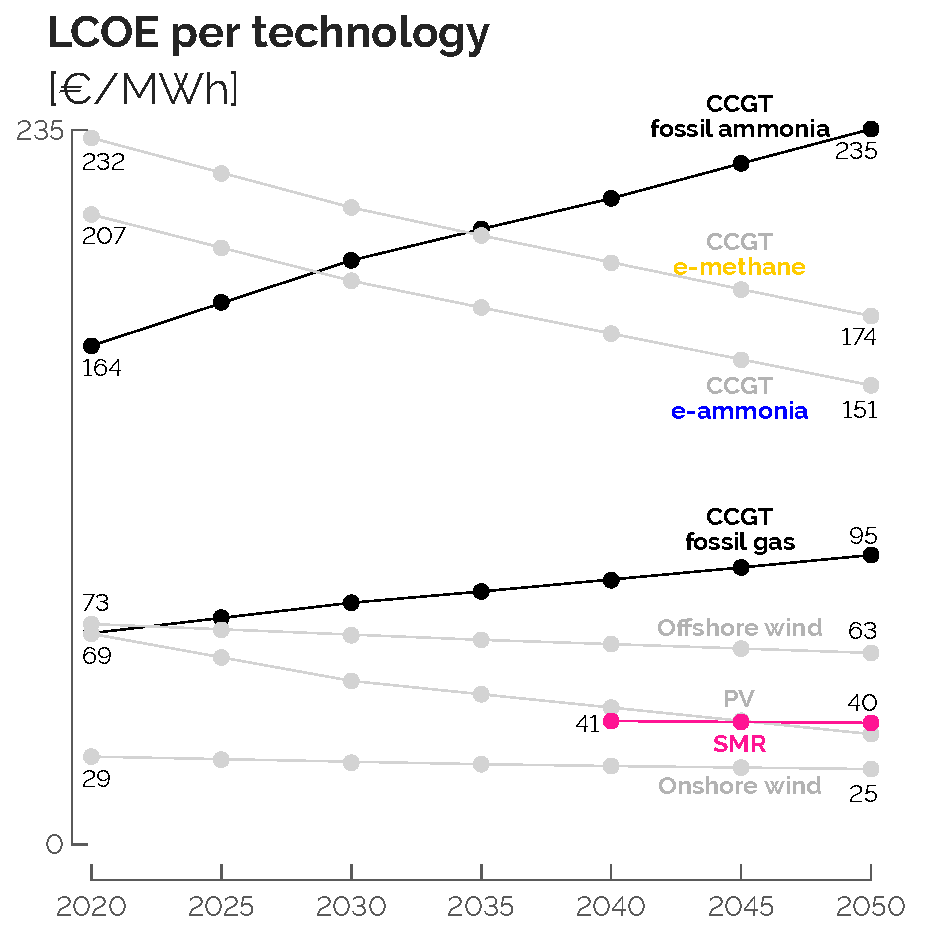
\includegraphics[width=0.49\textwidth]{LCOE_line_2.pdf}
\caption{Levelised cost of energy (LCOE) for the main technologies in the power sector. Gray and black curves are related to technologies runnning on renewable and fossil resources, respectively. Where \gls{SMR} is cheaper than the other flexible options, \gls{CCGT} running on e-ammonia is, a priori, cheaper than its e-methane alternative.}
\label{fig:LCOE}
\end{figure}

\subsection{Technologies supplying the non-energy demand}
\label{subsec:cs:NED_tech}

Different paths are implemented to produce the final molecules of the NED (see \Cref{fig:NED_tech}). Similarly to \citet{tsiropoulos2018emerging}, naphtha, here considered as \gls{LFO}, resulting from refinery operation is modeled as an imported commodity. Presented here for the specific year of 2035, all data and related references can be found in \cite{GIT_NED}. To keep the same level of details with other sectors of the model, the implementation of the conversion technologies consists of a single kind of technology per type of resource to produce a certain product. For instance, in the model, there is only one technology to produce \gls{HVC} either from naphtha or from LPG, two liquid fossil hydrocarbons, \ie \gls{NSC}. For ammonia and methanol, the molecules can either be produced locally from other resources or directly imported (with distinction between non-renewable and renewable molecules). 

\begin{figure}[htbp!]
\centering
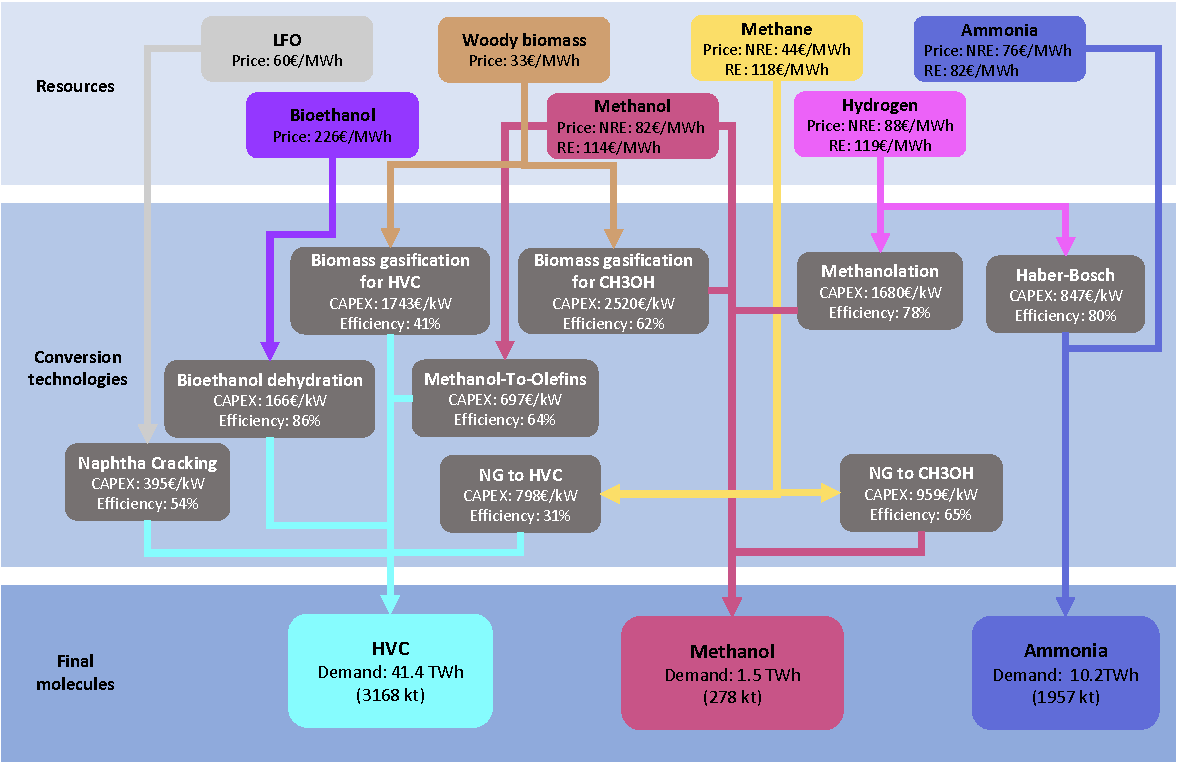
\includegraphics[width=0.8\textwidth]{NED_tech.pdf}
\caption{Schematic view of the different resources able to produce \gls{HVC}, ammonia and methanol with their related conversion technologies (including energy efficiency and their CAPEX - in €/kW of final molecules).  Values stand for 2035. Graph from \cite{rixhon2021comprehensive}}
\label{fig:NED_tech}
\end{figure}

\myparagraph{The impact of integrating the \gls{NED} in the Belgian whole-energy system}\\

\noindent
Works of \citet{rixhon2021comprehensive,rixhon2022integration} assessed the impact of the integration of the \gls{NED} in the case of Belgium, using EnergyScope TD (see Appendix \ref{app:ESTD}).  This snapshot model, \ie optimising the system in a target future year (\ie 2050 in this case) considering a green field approach, investigated the defossilisation of the system. To analyse the whole-energy system at different ``climate targets'', the model forced the total emissions to decrease by reducing their upper limit while optimising the total cost. In practice, 10\% steps of \gls{GWP} reduction were made from the ``reference scenario - 100\%''. This strategy gave the following points of analysis: 100\% (\ie cost-optimum with no limitation on the total \gls{GWP}), 90\%, 80\%, ..., down to 0\% (\ie  carbon-neutrality).\\

First and foremost, when the \gls{NED} is implemented with this higher level of details, we highlighted that woody biomass was ``cannibalised'' to produce methanol, instead of high-temperature heat, in the cost-optimum situation. At more ambitious ``climate targets'', e-methanol rises as the keystone to defossilise the \gls{NED} sector as \gls{MTO} becomes the favoured option to produce \gls{HVC}, representing the major share of the \gls{NED}. Then, including the \gls{NED} affects the selection of the technologies for the satisfaction of the heat and the electricity demands. The additional high-temperature demand required by the \gls{NED} forces the system to invest in more efficient technologies like \gls{CHP} instead of \gls{CCGT}. This additional heat demand mostly supplies naphtha-cracking substituted by \gls{MTO} at more ambitious ``climate targets'' to produce \gls{HVC}. To a lesser extent, to respect the emissions-caps, integrating the \gls{NED} leads to a higher integration of solar-\gls{PV} to support the electrification of the low-temperature heat sector.\\


For further details on these analyses, the interested reader is invited to refer to aforementioned for further published works.

\section{Uncertainty ranges}
\label{sec:cs:uncertainty}
As detailed in Section \ref{sec:meth:UQ}, accounting for uncertainty in \gls{ESOMs} is crucial \cite{mavromatidis2018uncertainty}, especially when it comes to optimise several decades in an inherently uncertain future. The fundamental step in this ambition is to characterise these uncertainties. In this work, following the approach of \citet{Moret2017PhDThesis}, we have defined range of uncertainties for the model parameters. \Cref{tab:UC_short} gives the uncertainty ranges of some key parameters. Like other works \cite{li2019renewables,coppitters2021robust}, the uncertain parameters are assumed to be independent and uniformly distributed between their respective lower and upper bounds. A particular attention is to pay to the potential installation of \gls{SMR}, at the bottom of \Cref{tab:UC_short}. As detailed before, the commercial availability of such a technology is uncertain but would not be before 2040. Consequently, for \gls{SMR}, the parameter $f_{\mathrm{max,SMR}}$ influences the maximum capacity to install to translate somehow the readiness of this technology. Arbitrarily, we have then assumed the following probability of availability of such a technology: 10\% of chance to be installable from 2040, 20\% from 2045 and 40\% from 2050\footnote{In other words, if this parameter, ranging between 0 and 1, is (i) smaller than 0.6, there is no possibility to install \gls{SMR} during the transition; (ii) between 0.6 and 0.8, these 6~GW can be installed only in 2050; (iii) between 0.8 and 0.9, these can be installed from 2045 onward and; (iv) higher than 0.9, the prescribed maximum capacity can be installed from 2040 onward. }. Based on the local sensitivity analysis carried out by \citet{PATHS2050}, the current work also considers a [-40\%; +44\%] range on the CAPEX of SMR, on top of the uncertainty about the availability. Finally, the the cost of purchasing renewable electrofuels presents a wide range, [-64.3\%; +179.8\%], like the other imported commodities.

The exhaustive list of the parameters accounted in this work is presented in Appendix \ref{app:UC_full}.

\begin{table}[htbp!]
\caption{Illustration of the uncertainty characterisation for different parameters for the year 2025. }
\label{tab:UC_short}
\begin{minipage}{\linewidth}
\centering
\resizebox{\textwidth}{!}{
\begin{tabular}{l l l c c c}
\toprule
\multirow{2}{*}{\textbf{Category}} & \multirow{2}{*}{\textbf{Parameter}} & \multirow{2}{*}{\textbf{Meaning}} & \multirow{2}{*}{\textbf{Type}\footnote{\label{foot:type_uncert_range}Per \citet{Moret2017PhDThesis}, \og I: investment-type, II: operation-type (constant uncertainty over time), III: operation-type (uncertainty increasing over time)\fg. }}  & \multicolumn{2}{c}{\textbf{Relative variation\footnote{\label{foot:nom_val_uncert}The nominal values of each of the parameters is 0, meaning no variation compared to the nominal values of the impacted parameter in the model. }}}\\
    & & & &	 min 	&	 max \\ 	
\midrule		
\multirow{2}{*}{\textbf{Cost of purchasing}} & $c_{\mathrm{op,fossil}}$ & Purchase fossil fuels & II & -64.3\% & 179.8\% \\
& $c_{\mathrm{op,electrofuels}}$ & Purchase electrofuels & II & -64.3\% & 179.8\% \\
\midrule
\multirow{5}{*}{\textbf{Investment cost}} &$c_{\mathrm{inv,car}}$ & CAPEX car  & I & -21.6\% & 25.0\% \\
& $c_{\mathrm{inv,e\_prop}}$ & CAPEX electric motor & I & -39.6\% & 39.6\% \\
& $c_{\mathrm{inv,fc\_prop}}$ & CAPEX fuel cell engine & I & -39.6\% & 39.6\% \\
& $c_{\mathrm{inv,PV}}$ & CAPEX PV & I & -39.6\% & 39.6\% \\
& $c_{\mathrm{inv,nuclear\_SMR}}$ & CAPEX \gls{SMR}\footnote{\label{foot:range_SMR}This range has been inferred from the local sensitivity analysis performed by \citet{PATHS2050}.}& I & -40.0\% & 44.0\% \\
\midrule
\multirow{1}{*}{\textbf{Consumption}} &$\eta_{\mathrm{e\_prop}}$ & Consumption electric vehicles & I & -28.7\% & 28.7\% \\
\midrule
\multirow{2}{*}{\textbf{Potential installed capacity}} &$f_{\mathrm{max,PV}}$ & Max capacity PV & I & -24.1\% & 24.1\% \\
& $f_{\mathrm{max,windon}}$ & Max capacity onshore wind & I & -24.1\% & 24.1\% \\
\midrule
\multirow{2}{*}{\textbf{Hourly load factor}} & $c_{\mathrm{p,t,PV}}$ & Hourly load factor PV & II & -22.1\% & 22.1\% \\
& $c_{\mathrm{p,t,winds}}$ & Hourly load factor wind turbines & II & -22.1\% & 22.1\% \\
\midrule
\multirow{2}{*}{\textbf{Resource availability}} & $avail_{\mathrm{elec}}$ & Available electricity import & I & -32.1\% & 32.1\% \\
& $avail_{\mathrm{biomass}}$ & Available local biomass & I & -32.1\% & 32.1\% \\
\midrule

\multirow{2}{*}{\textbf{End-use demand}} & $pass\_EUD$ & Passenger mobility EUD & III & -7.5\% & 7.5\% \\
& $industry\_EUD$ & Industry EUD & III & -20.5\% & 16.0\% \\
\midrule

\multirow{4}{*}{\textbf{Miscellaneous}} &$i_{\mathrm{rate}}$  & Interest rate & I & -46.2\% & 46.2\% \\
& $\Delta_{\mathrm{change,freight}}$ & Modal share change freight mobility & - & -30\% & 30\% \\
& $\Delta_{\mathrm{change,pass}}$ & Modal share change passenger mobility & - & -30\% & 30\% \\
& $f_{\mathrm{max,SMR}}$ & Potential capacity \gls{SMR} & - & 0 & 1 \\

\bottomrule							

\end{tabular}}
\end{minipage}
\end{table}

\section{\ce{CO2}-budget for the transition}
\label{sec:cs:CO2-budget}
In most of the studies carried out on the pathway optimisation of a whole-energy system, a \ce{CO2}-trajectory is \textit{a priori} set to reach carbon-neutrality by 2050. \citet{nerini2017myopic} used the emission trajectory indicated by the UK's Committee on Climate Change in their analysis of the impact of limited foresight to achieve the target of 80\% reduction of \gls{GHG} by 2050 in the United Kingdom. In their assessment of the impacts of economy-wide emissions policies in the water-energy-land nexus, \citet{licandeo2023assessing} analysed different \ce{CO2}-trajectories considering more or less severe water scarcity for the US. \citet{poncelet2016myopic} with LUSYM (Leuven University SYstem Model) and \citet{PATHS2050} with TIMES-BE also set decreasing emission trajectories in their analysis of respectively the Belgian power sector and whole-energy system.  Others only set the objective as the carbon-neutrality by 2050. For instance, \citet{heuberger2018impact} investigated the impact of different factors (\eg limit of the foresight in the future, availability of \og unicorn technologies\fg or committed versus market-driven decarbonisation strategies) to reach this ultimate objective in the UK system.\\

In this work, the effect of greenhouse gases is cumulative over time and a constraint is set on the overall emissions of the transition---a \ce{CO2}-budget for the transition. This approach is in line with the works defining safe operating spaces within the nine different global planetary boundaries (\ie (i) novel entities, (ii) stratospheric ozone depletion, (iii) atmospheric aerosol loading, (iv) ocean acidification, (v) biogeochemical flows, (vi) fresh water change, (vii) land system change, (viii) biosphere integrity, and, (ix) climate change) \cite{richardson2023earth,steffen2015planetary,rockstrom2009safe}. This ``systemic framework for addressing global anthropogenic impacts on Earth system'' gives quantitative recommendations about the \ce{CO2} concentration, among others, to maintain ``the stability and resilience of Earth system as a whole'' \cite{richardson2023earth}. In their review, \citet{ryberg2020downscaling} identified three main sharing principle categories when considering these safe spaces: \ie \textit{utilitarian}, \textit{egalitarian} and \textit{acquired rights} principles.In a nutshell, the former, mostly applied to the scale of industry sector \cite{ryberg2018bring,brejnrod2017absolute}, aims at maximising the sum of welfare. The second shares the so-called ``budget'' equally among the total population, allocating the same share to each individual \cite{hoff2017bringing,o2018good}. Finally, in \textit{acquired rights} principles, also called ``grandfathering'', the sharing is based on \og maintaining that prior emissions increase future emission entitlements\fg  \cite{knight2013grandfathering}.In this thesis, we have chosen the latter principle to allocate the \ce{CO2}-budget to the Belgian transition. This budget (1.2\,Gt$_{\ce{CO2},\text{eq}}$) corresponds to the proportion of Belgium's emissions in the world emissions in 2020 (34.8\,Gt$_{\ce{CO2},\text{eq}}$ \cite{ourworldindata_CO2_world}) applied to the global budget to have a 66\% chance of limiting warming to 1.5°C of 420\,Gt$_{\ce{CO2},\text{eq}}$ \cite{IPCC_CO2_budget}. Therefore, in this work, a limit has been put on $\emph{gwp\textsubscript{lim,trans}}=1.2\,\text{Gt}_{\ce{CO2},\text{eq}}$ in Eq.\,(\ref{eq:limit_gwp_trans}). This is another sign of the urgency to act to mitigate climate change as this 30-year budget represents only 10 years of the current emissions. \\

Compared to a linear decrease from the current emissions, as done by \citet{limpens2024pathway}, this budget represents a 60\% reduction of the cumulative emissions over the transition.  Appendix \ref{app:CO2_budget} compares the emissions trajectory between the REF case and a case (without \gls{SMR}) where the linear decrease is imposed between 2020 and carbon-neutrality in 2050.
\clearpage

%%% -- Chapter 3 - Myopic implementation on the pathway optimisation -----------------------------
%\clearemptydoublepage
%\chapter{From a perfect foresight to a myopic optimisation of the pathway} 
%\label{chap:chap_myopic}
%%!TEX root = ../thesis_main.tex
%!TEX encoding = UTF-8 Unicode
In this chapter, I highlight the advantages of the myopic pathway, the methodological adaptations needed to have a myopic optimisation from EnergyScope Pathway perfect foresight and detail the difference with the perfect foresight for the case study. 

\section{Why and how myopic}
\label{sec:chap3_why_how}
Besides the fact that it is a necessary framework for the application of RL,  explain here why it is interesting, as is, to consider myopic optimisation (time saving, more appropriate to mimic policymakers' shortsightedness, etc.)

Detail the little tweeks to go from a perfect foresight to a myopic optimisation, in terms of implementation.

\section{Case study and results: Belgian energy system under \ce{CO2} trajectory}
\label{sec:chap3_case_study_results}

\subsection{Case study}
{\color{red}Question to HJ and FC : J'hésite sur le cas de référence pour la comparaison en termes de trajectoire \ce{CO2}. Voici ce à quoi je pense:
\begin{enumerate}
\item Comme ce qu'on a présenté dans le papier Pathway, une décroissance linéaire entre les émissions de 2020 et la neutralité carbone en 2050
\item Sur base du budget \ce{CO2} identique à celui de la décroissance linéaire (~1.9Gt\ce{CO2}), imposer au myopique la trajectoire \ce{CO2} issue de l'optimisation perfect foresight. Dans cette option, il y a deux sous-choix:
\begin{itemize}
\item Imposer la neutralité carbone en 2050, comme dans le cas 1.
\item Ne pas imposer la neutralité carbone en 2050
\end{itemize}
\item Sur base du budget \ce{CO2} que je donne implicitement comme objectif à mon agent (~1.2Gt\ce{CO2}), imposer au myopique la trajectoire \ce{CO2} issue de l'optimisation perfect foresight. Dans cette option, il y a deux sous-choix:
\begin{itemize}
\item Imposer la neutralité carbone en 2050, comme dans le cas 1.
\item Ne pas imposer la neutralité carbone en 2050
\end{itemize}
\end{enumerate}
Perso, je choisirais de me rapprocher le plus possible de ce que je fais ensuite avec l'agent. Du coup, ce serait le cas 3  sans imposer la neutralité carbone 2050. Dans ce cas, pour l'avoir observé, le modèle n'atteint pas la neutralité carbone. 

Quel est votre avis sur la question?
}

Define the case study and the \ce{CO2} trajectory. 

\subsection{Results and comparison with Perfect foresight}

\subsection{Discussion and perspective with the literature} 
%\clearpage


%% -- Chapter 4 - Reinforcement Learning -
%\clearemptydoublepage
%\chapter{Reinforcement Learning \ce{CO2}-policy robust optimisation}
%\label{chap:chap_RL}
%\vspace{-0.2cm}
\begin{flushright}
\emph{``For the things we have to learn before we can do them, we learn by doing them.''}\\
Aristotle, in \textit{The Nicomachean Ethics}, IV$^\text{th}$ century BC
\end{flushright}
\vspace{0.4cm}

Uncertainties about the future along with a large variety of \gls{IAMs} yield an even larger variety of \gls{GHG} emissions reduction pathways \cite{nicolas2021robust}. For instance, several studies \cite{IPCC_CO2_budget,steffen2018trajectories} advocate for actions to take in the near future, especially to keep on track within the 1.5°C (if not, 2°C) increase of global temperature above pre-industrial levels by the end of the century. On the contrary, using his top-down model DICE, \citet{nordhaus2014question} states that immediate and drastic actions are not compulsory to meet the ambition of climate change mitigation. 

To navigate through the myopic transitions not constrained by a prescribed \ce{CO2}-trajectory and investigate the efficiency of different policies, we apply the reinforcement learning approach detailed in Section \ref{sec:meth:RL} on the case study of Belgium. Besides the environment, \ie the myopic transition pathway of the whole-energy system via EnergyScope Pathway (see Chapter \ref{chap:chap_methodo}), the first part of this chapter presents the three key features of interaction between the agent, optimizing its policy, and the environment: actions, states and reward.  Then, the results of this policy optimisation point out strategies to follow, \ie \textit{sweet spots}, in the transitions under uncertainties as well as \textit{no-go zones} where the chances of succeeding the transition, \ie respecting the \ce{CO2}-budget, are very limited. Finally, these results are compared with references, \ie the perfect foresight and the myopic optimisation of the transition under the same uncertainties but without the trained \gls{RL}-agent that can support this transition thanks to its learned policy.

\section*{Contributions}
\label{sec:RL:contributions}
Applying the \gls{RL} approach to the optimization of the myopic transition pathway of a whole-energy system presents several novelties. First of all, as introduced in Section \ref{subsec:meth_RL_fundamentals}, when applied to energy systems, \gls{RL} is more dedicated either to smaller scale systems (\eg \gls{BEMS}, vehicles and energy devices) or to sector-specific, often the power sector, problems (\eg dispatch problems, energy markets and grid) \cite{perera2021applications}. In our case, the sector-coupling, the long-term goal at the end of a multiple-steps transition and the number of uncertain parameters make this application new for \gls{RL}.

Applying \gls{RL} to the optimisation environment of EnergyScope Pathway myopic,  rather than a simulation environment, allows building a hierarchical multi-objective optimisation framework: while the objective of the environment remains the minimisation of the total ``transition'' cost (on the concerned limited time window), the agent optimises its strategy to respect the \ce{CO2}-budget. 

Comparing the \gls{RL}-based results with more conventional approaches, \ie perfect foresight optimisation, highlights the added-value brought by this approach in the exploration of myopic transition pathways.

Usually, applications of \gls{RL} focus more on the result of the learning process, the optimised policy, for optimising the control of a system \cite{perera2021applications}. This thesis also investigates the learning episodes themselves to explore the field of possibilities to succeed the transition.


\section{Definition of the actions, reward and states}
\label{sec:RL:act_states_rew}
As already introduced in Section \ref{subsec:meth_RL_algo}, the environment with which the \gls{RL}-agent interacts is the optimisation of the transition pathway of a whole-energy system on a specific time window, \eg 2020-2030 then 2025-2035 and so on, until 2040-2050 (see Figure \ref{fig:Schematics_RL}). In a nutshell, starting from the initial state of the environment (\ie the whole-energy system in 2020), the agent takes a set of actions that influence the environment, \ie that affects parameters of the Linear Programming in EnergyScope Pathway. Then, the window 2020-2030 is optimised via EnergyScope. Some of the outputs of this optimisation feed the agent with either the new state of the system or the reward, \ie telling the agent how good the actions were at the state he took it. Based on the new state and the reward, the agent takes another set of actions and the window 2025-2035 is optimised. This goes on until 2050.

\subsection{Actions}
\label{subsec:RL:act_states_rew:act}

Defining the levers of action, the core of the policy, to support the transition of a country-size whole-energy system is challenging, especially when accounting for political and socio-technical aspects \cite{castrejon2020making}. In our work, focusing only on the techno-economic aspect, we assume that the actions taken by the agent are directly implemented and impacting the environment. In other words, considering only the techno-economic lens, there is no moderation nor contest towards the agent's actions, as the objective is to assess how far and when within the transition to push the different levers of action. Given the overall objective of the agent to succeed the transition, \ie respecting the \ce{CO2}-budget by 2050, we have defined the actions in this sense. The first action, $\mathrm{act}_{\mathrm{gwp}} \in [0,1]$, aims at limiting the emissions at the representative year ending the concerned time window, $\textbf{GWP\textsubscript{tot}}(y_{\text{end of the window}})$, between the level of emissions in 2020, \ie $\textbf{GWP\textsubscript{tot}}(2020)=123\,\text{Mt}_{\ce{CO2},\text{eq}}$, and carbon-neutrality:

\begingroup
\belowdisplayskip=2pt
\abovedisplayskip=2pt
\begin{flalign} 
\label{eq:RL:act_gwp}
&\textbf{GWP\textsubscript{tot}}(y_{\text{end of the window}})\leq \mathrm{act}_{\mathrm{gwp}} \cdot \textbf{GWP\textsubscript{tot}}(2020). &
\end{flalign}
\endgroup

\noindent
This action is equivalent to setting a national \ce{CO2}-quota.

Three additional actions support the strict limitation of yearly emissions: limiting the consumption of oil, fossil gas and coal. Out of the total \gls{GHG} emissions in Belgium in 2020, oil (\ie so-called ``\gls{LFO}'' in the model) and fossil gas account for roughly 40\% and 31\%, respectively. In 2020, solid fossil fuels (\ie so-called ``coal'' in the model) is much less consumed than oil and gas: \ie 28\,TWh of solid fossil fuels versus 159 and 142\,TWh for oil and fossil gas, respectively. Even though its cost (17€/MWh) makes coal cost-competitive, it is a highly-emitting resource, 0.40\,kt$_{\ce{CO2},\text{eq}}$/GWh. For these reasons, three independent actions limit the consumption of these three fossil resources up to the level of consumption in 2020, $\textbf{Cons\textsubscript{fossil gas}}(2020)$, $\textbf{Cons\textsubscript{LFO}}(2020)$ and $\textbf{Cons\textsubscript{coal}}(2020)$,  over the entire concerned time window, except the first one as this year is the initial condition of the time window and cannot be optimised any more:

\begingroup
\belowdisplayskip=2pt
\abovedisplayskip=2pt
\begin{flalign} 
\label{eq:RL:act_NG}
&\textbf{Cons\textsubscript{fossil gas}}(y)\leq \mathrm{act}\textsubscript{fossil gas} \cdot \textbf{Cons\textsubscript{fossil gas}}(2020) & \forall y \in \text{time window}\\
\label{eq:RL:act_LFO}
&\textbf{Cons\textsubscript{LFO}}(y)\leq \mathrm{act}\textsubscript{LFO} \cdot \textbf{Cons\textsubscript{LFO}}(2020) & \forall y \in \text{time window}\\
\label{eq:RL:act_COAL}
&\textbf{Cons\textsubscript{coal}}(y)\leq \mathrm{act}\textsubscript{coal} \cdot \textbf{Cons\textsubscript{coal}}(2020) & \forall y \in \text{time window}
\end{flalign}
\endgroup

\noindent
where $\mathrm{act}\textsubscript{fossil gas}$, $\mathrm{act}\textsubscript{LFO}$ and $\mathrm{act}\textsubscript{coal}$ can take values between 0 and 1. These complete the action space of the agent, $A\in \mathbb{R}^4_{[0,1]}$.

\subsection{Reward}
\label{subsec:RL:act_states_rew:rew}

When the reward is not properly defined, the agent may optimise its policy for an unintended objective, leading to undesired or subotpimal behavior, \ie the so-called misalignment of the learning objective \cite{christiano2017deep}. Even worse, it can lead to reward hacking (or reward tampering) where the agent exploits loopholes in the reward function to achieve higher rewards without actually performing the desired task \cite{amodei2016concrete}. On the contrary, a proper definition of the reward function increases the sample efficiency, \ie requiring less episode to converge to the optimal policy.  It also makes the policy more stable and able to withstand variations and uncertainties in the environment \cite{henderson2018deep}.

Through its maximisation of the expected return (see Section \ref{subsec:meth_RL_algo}), a \gls{RL}-agent is as sensitive to positive reward, \ie the carrot, as negative reward, \ie the stick.  When the former encourages desired behaviours, the latter can be seen as a penalty or a punishment and discourages the undesirable behaviours \cite{sutton2018reinforcement}. In our case, we have decided to combine these two approaches (see Figure \ref{fig:Reward}).

\begin{figure}[!htbp]
\centering
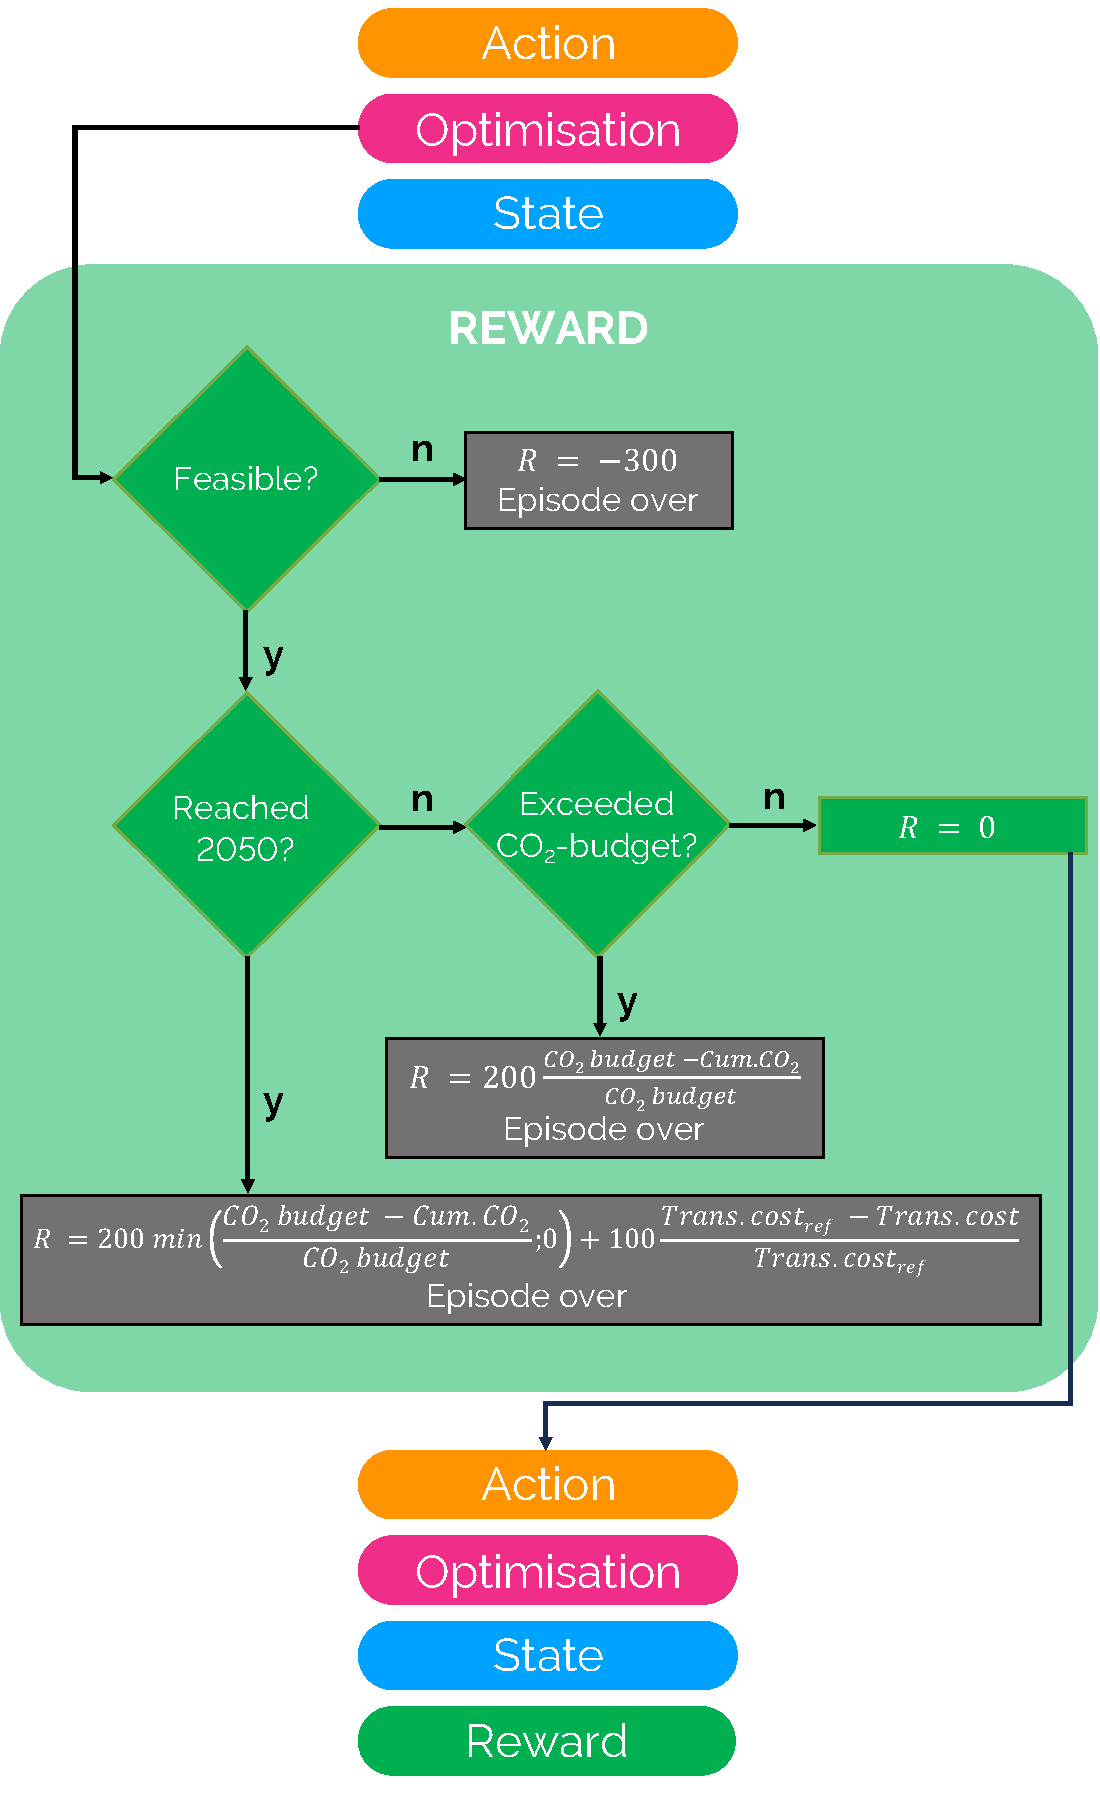
\includegraphics[width=0.8\textwidth]{Reward.pdf}
\caption{Reward function, $R$. Before reaching 2050, the episode is prematurely ended and a negative reward is given if the optimisation is infeasible or if the \ce{CO2}-budget is exceeded. If the optimisation provides a solution and the \ce{CO2}-budget is not exceeded, the episode continues. Finally, if the episode goes until 2050, the reward is a weighted sum between the capped cumulative emissions and the total transition cost.}
\label{fig:Reward}
\end{figure} 

The reward function is defined in three steps. First of all, taking a set of actions at a certain state might lead to an infeasible optimisation problem. In other words, as actions have a direct impact on some constraints of the problem, they might limit too much the feasible domain to the point where no solution can be found. For instance, the extreme case of aiming at carbon-neutrality, \ie $\mathrm{act}_{\mathrm{gwp}}=0$, and forbidding the use of the three aforementioned fossil fuels, \ie $\mathrm{act}\textsubscript{fossil gas}=\mathrm{act}\textsubscript{LFO}=\mathrm{act}\textsubscript{coal}=0$,  from the beginning of the transition makes the optimisation impossible to solve. In this case, the episode is prematurely ended and the reward is ``highly'' negative, -300. If the optimisation is feasible and the end of the transition, \ie 2050, is not reached, the cumulative emissions so far are evaluated. On the one hand, if these cumulative emissions exceed the \ce{CO2}-budget, $1.2\,\text{Gt}_{\ce{CO2},\text{eq}}$ (see Section \ref{sec:cs:CO2-budget}), the episode is also ended and a penalisation is given to the agent. This penalisation is proportional to the difference between the \ce{CO2}-budget and the actual cumulative emissions.  On the other hand, the episode continues with a zero reward if the \ce{CO2}-budget is not exceeded. Eventually, when reaching 2050, given the main objective of the agent to respect the \ce{CO2}-budget and not to be more ``\ce{CO2}-ambitious'', we cut short the contribution of the cumulative emissions as soon as they are lower or equal to the \ce{CO2}-budget.  On top of that, the reward function includes a secondary objective: the cumulative transition cost. To make the agent sensitive to the cost-impact of its policy, we added the total transition cost in the reward function where the \emph{Trans. cost$_{\text{ref}}$} on Figure \ref{fig:Reward} is equal to $1.1\cdot10^3$\,b€. This value comes from the mean of the total transition costs obtained through the \gls{GSA} performed on the perfect foresight transition pathway optimisation (see Section \ref{subsec:atom_mol:results_uq_cost}). In this final form of the reward, one will notice that overshooting cumulative emissions are more penalising than an overshooting transition cost, \ie weight of 200 for the emissions versus 100 for the cost. The values of these weights are the results of a trial and error to fine-tune the balance between more expensive successes and cheaper failures. This way, we observed that the agent first targeted the respect of the \ce{CO2}-budget and then, to a lesser scale, avoided reaching over-costly transitions.

\subsection{States}
\label{subsec:RL:act_states_rew:states}

Besides the reward, states are the other piece of information provided by the environment to the agent. In \gls{RL}, the purpose of states are to represent the current situation or configuration of the environment in which the agent operates. The primary function of states in RL is to provide the necessary context for the agent to choose appropriate actions based on its current observations and goals \cite{sutton2018reinforcement}. The challenge in the definition of the states is to provide enough information but not too much to avoid overwhelming the agent with non-informative features. 

Consequently, after testing several state spaces and observing the convergence of the reward, we have converged to a four-dimension state space characterizing the energy system at the end of the optimised time window. The first dimension is directly related to the main objective of the agent: respecting the \ce{CO2}-budget until 2050. Therefore, the cumulative emissions emitted so far up to the current step of the transition is the first dimension of the states. Similarly, the cumulative cost of the transition so far constitutes the second dimension of the states to inform the agent about the cost-impact of its actions on the environment. Finally, to enrich the level of details, we have added two other dimensions representative of the key-to-the-transition indicators identified in the Renewable Energy Directive (RED) III of the European Commission \cite{REDIII}: the share of renewables in the primary energy mix and, the energy efficiency. The former is computed as the share of local renewables (\ie wind, solar, hydro and biomass) and imported renewable energy carriers (\ie biofuels and electrofuels) in the total consumption of primary energy. Electricity imported from abroad is not considered in the set of renewable energy carriers even if it can be assumed to be fully renewable by 2050. Finally, even though energy efficiency is usually defined as the ratio between the \gls{FEC} and the primary energy mix, we decided to define this efficiency with a focus on the \gls{EUD}, like in the rest of this thesis. Where electricity, heat and non-energy \gls{EUD} are expressed in terms of energy content, we needed to convert passenger and freight transports into their respective \gls{FEC} to integrate them in the ratio. The information of efficiency fed back by the environment to the agent is the ratio between a ``hybrid'' \gls{EUD} and the consumption of primary energy resources.

\section{Convergence and learning process}
\label{sec:RL:learning}

Before comparing the agent's optimised policy with references, the first step consists in assessing the learning of the \gls{NN}, also called ``training''. For this, numerous episodes are played through the myopic optimisation of the transition pathway of Belgium. At the beginning of each episode, the agent starts with the Belgian energy system of 2020 (see Appendix \ref{app:bel_2020}). Then, a sample of values, drawn for the uncertain parameters, affects the model for the 2020-2030 time window. This single draw will affect the parameters for all the subsequent time windows (see Figure \ref{fig:ranges_transition}).  Then, the agent takes a set of actions, affecting the environment that feeds back the agent with a new state and a reward. This goes on until the end of the episode. For the next episode, similarly to the \gls{UQ} analysis (see Section \ref{sec:meth:UQ}), another sample of uncertain parameters is drawn following the quasi-random Sobol' sampling technique \cite{bratley2003implementing}.

\subsection{Reward and success}
\label{subsec:RL:learning:rew_succ}

The learning phase has been split into batches of 500 steps. %For the first 100 steps of each batch, the \gls{RL}-model collects transitions before learning starts. This makes sure replay buffer is full enough for useful updates. 
At the end of each batch, the up-to-date policy, \ie the \gls{NN}, is saved. This way, we can assess the progress in the learning process and its convergence (see Figure \ref{fig:reward_success}).  The mean reward increases rapidly at the beginning of the learning process before reaching a plateau where the optimisation of the policy becomes more marginal.  As this successes drive indirectly the agent's optimisation, it shows that the reward function (see Figure \ref{fig:Reward}) leads towards more and more successes. However, given the wide range of uncertainty of some parameters and the agent's levers of action, this success rate stays limited at the end of the learning process. In other words, there are conditions where it is impossible for the agent to succeed the transition.

\begin{figure}[!htbp]
\centering
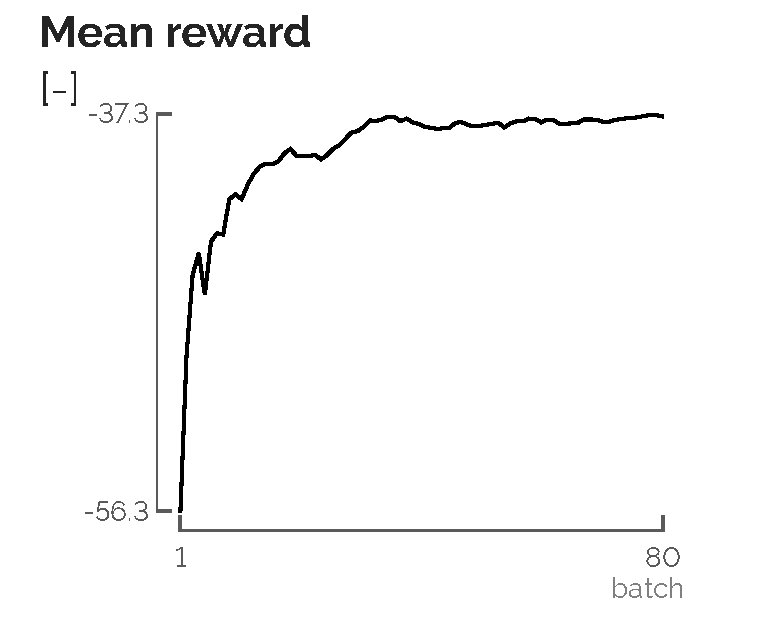
\includegraphics[width=0.49\textwidth]{Mean_reward.pdf}
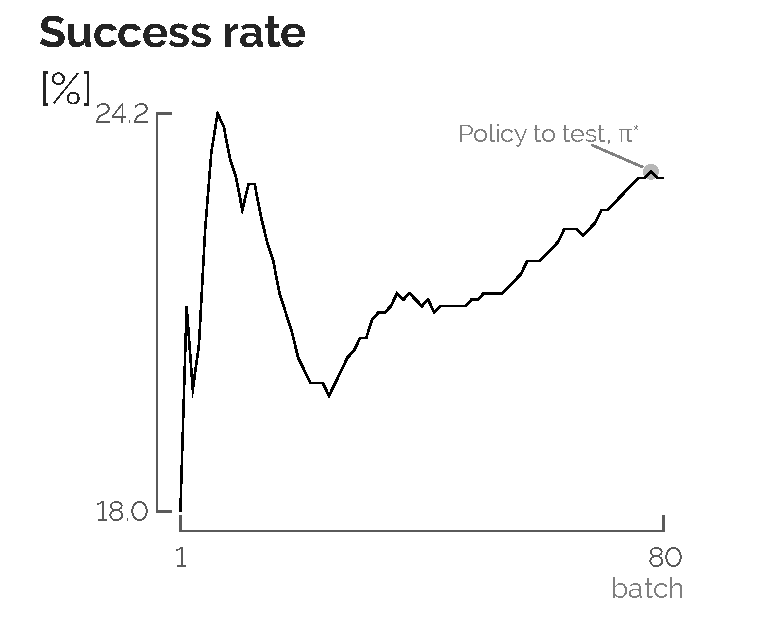
\includegraphics[width=0.49\textwidth]{Success_rate.pdf}
\caption{Mean reward and success rate of the different learning batches. The stabilisation of the reward curve shows a convergence of the learning process for the agent's point of view. The evolution of the success rate also shows that the reward function aims at more and more successful transitions.}
\label{fig:reward_success}
\end{figure}

\newpage
During the learning process, the algorithm explored numerous transition pathways: 2,037 successful transitions out of 10,751 attempts. 2\% of the total attempts led to infeasible optimisation of the initial time window. On top of that, each pathway provides valuable insight into the possible alternatives --- the primary goal of reinforcement learning. As a side benefit, the collection of all explored pathways also identifies the intermediate milestones to reach and the range of actions that must be avoided or must be taken. Yet, the exploration during this learning process is not exhaustive. The trends provided below are therefore not proven. The randomness of the process and the number of explored transition pathways still give high confidence in the conclusions drawn from these analyses.

There is a range in the reward where failures and successes overlap (see Figure \ref{fig:reward_status}). This area corresponds to either transitions that exceed the \ce{CO2}-budget in 2050 but are cheaper than the total transition cost of reference (see Section \ref{sec:RL:act_states_rew}) or successful transitions that are more expensive. Besides this overlap, we observe that successes account for the majority of the cases where the reward is positive. This is another indication that the reward function is appropriate in this exploration of successful transition pathways. More indirectly, this substantiates that the weights between emissions and cost defined in Section \ref{subsec:RL:act_states_rew:rew} could be used and adapted for another case study.

\begin{figure}[!htbp]
\centering
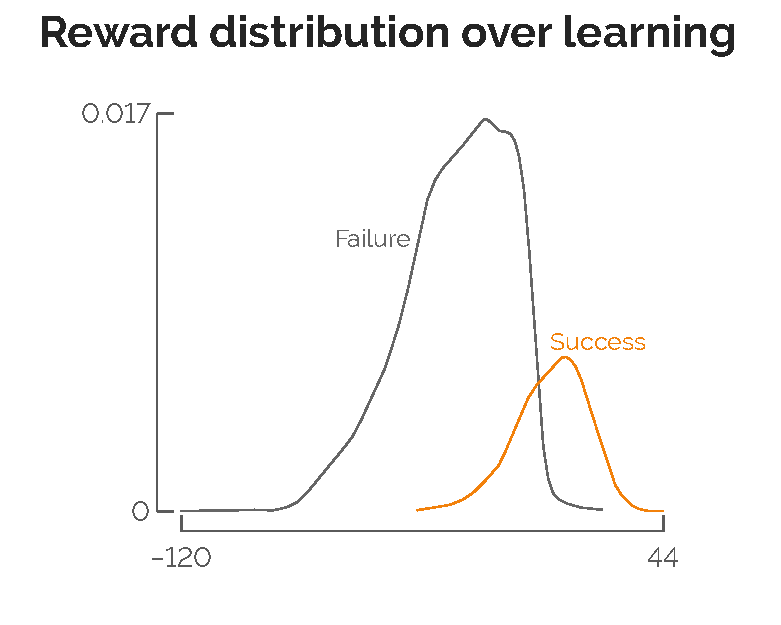
\includegraphics[width=0.49\textwidth]{Reward_status.pdf}
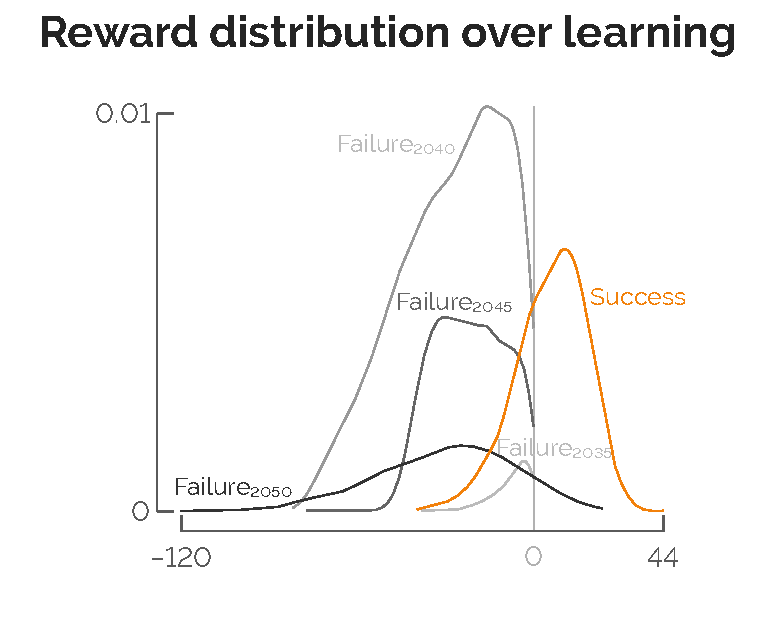
\includegraphics[width=0.49\textwidth]{Reward_status_2.pdf}
\caption{Reward distribution between successes and failures. Right hand side details at the end of which time-window the failure occurred. The ``tipping year'' is 2040 as failing the transition by 2040 represents 57\% of all the failures. Beyond this point, through this learning process, succeeding the transition represents 38\% of the episodes. }
\label{fig:reward_status}
\end{figure}

\newpage
Considering the end of the time-window where the \ce{CO2}-budget is exceeded, the right hand side of Figure \ref{fig:reward_status} shows that 2040 is the ``tipping year'' for the agent. Beyond this point, through this learning process, the chances to succeed the transition were 38\%. In other words, near-term (2025-2030) actions are necessary to hope succeeding the transition.

\subsection{States}
\label{subsec:RL:learning:states}

The first two dimensions of the state space are the cumulative emissions and costs. They drive the value of the reward and, consequently, the optimisation of the agent's policy. Per definition, the threshold of 1.2\,Gt$_{\ce{CO2},\text{eq}}$ splits the episodes reaching 2050 into successes and failures (see Figure \ref{fig:Cum_gwp_cost}). In the successful transitions, the median cumulative emissions, $\text{P}_{50}$, are about 0.9\,Gt$_{\ce{CO2},\text{eq}}$. Reaching cumulative emissions significantly lower than the \ce{CO2}-budget are possible thanks to efforts made at earlier stages of the transition and the potential to install \gls{SMR} later on. Considering the failures, half of these episodes ended up with cumulative emissions lower or equal to 1.4\,Gt$_{\ce{CO2},\text{eq}}$. As illustrated in Figure \ref{fig:reward_status}, 2040 is identified as the tipping year. Where 98\% of the failures were below the \ce{CO2}-budget in 2035, only 37\% passed this threshold in 2040. This reminds the importance of near-term, 2025-2030, actions to hope for a successful transition.

\begin{figure}[!htbp]
\centering
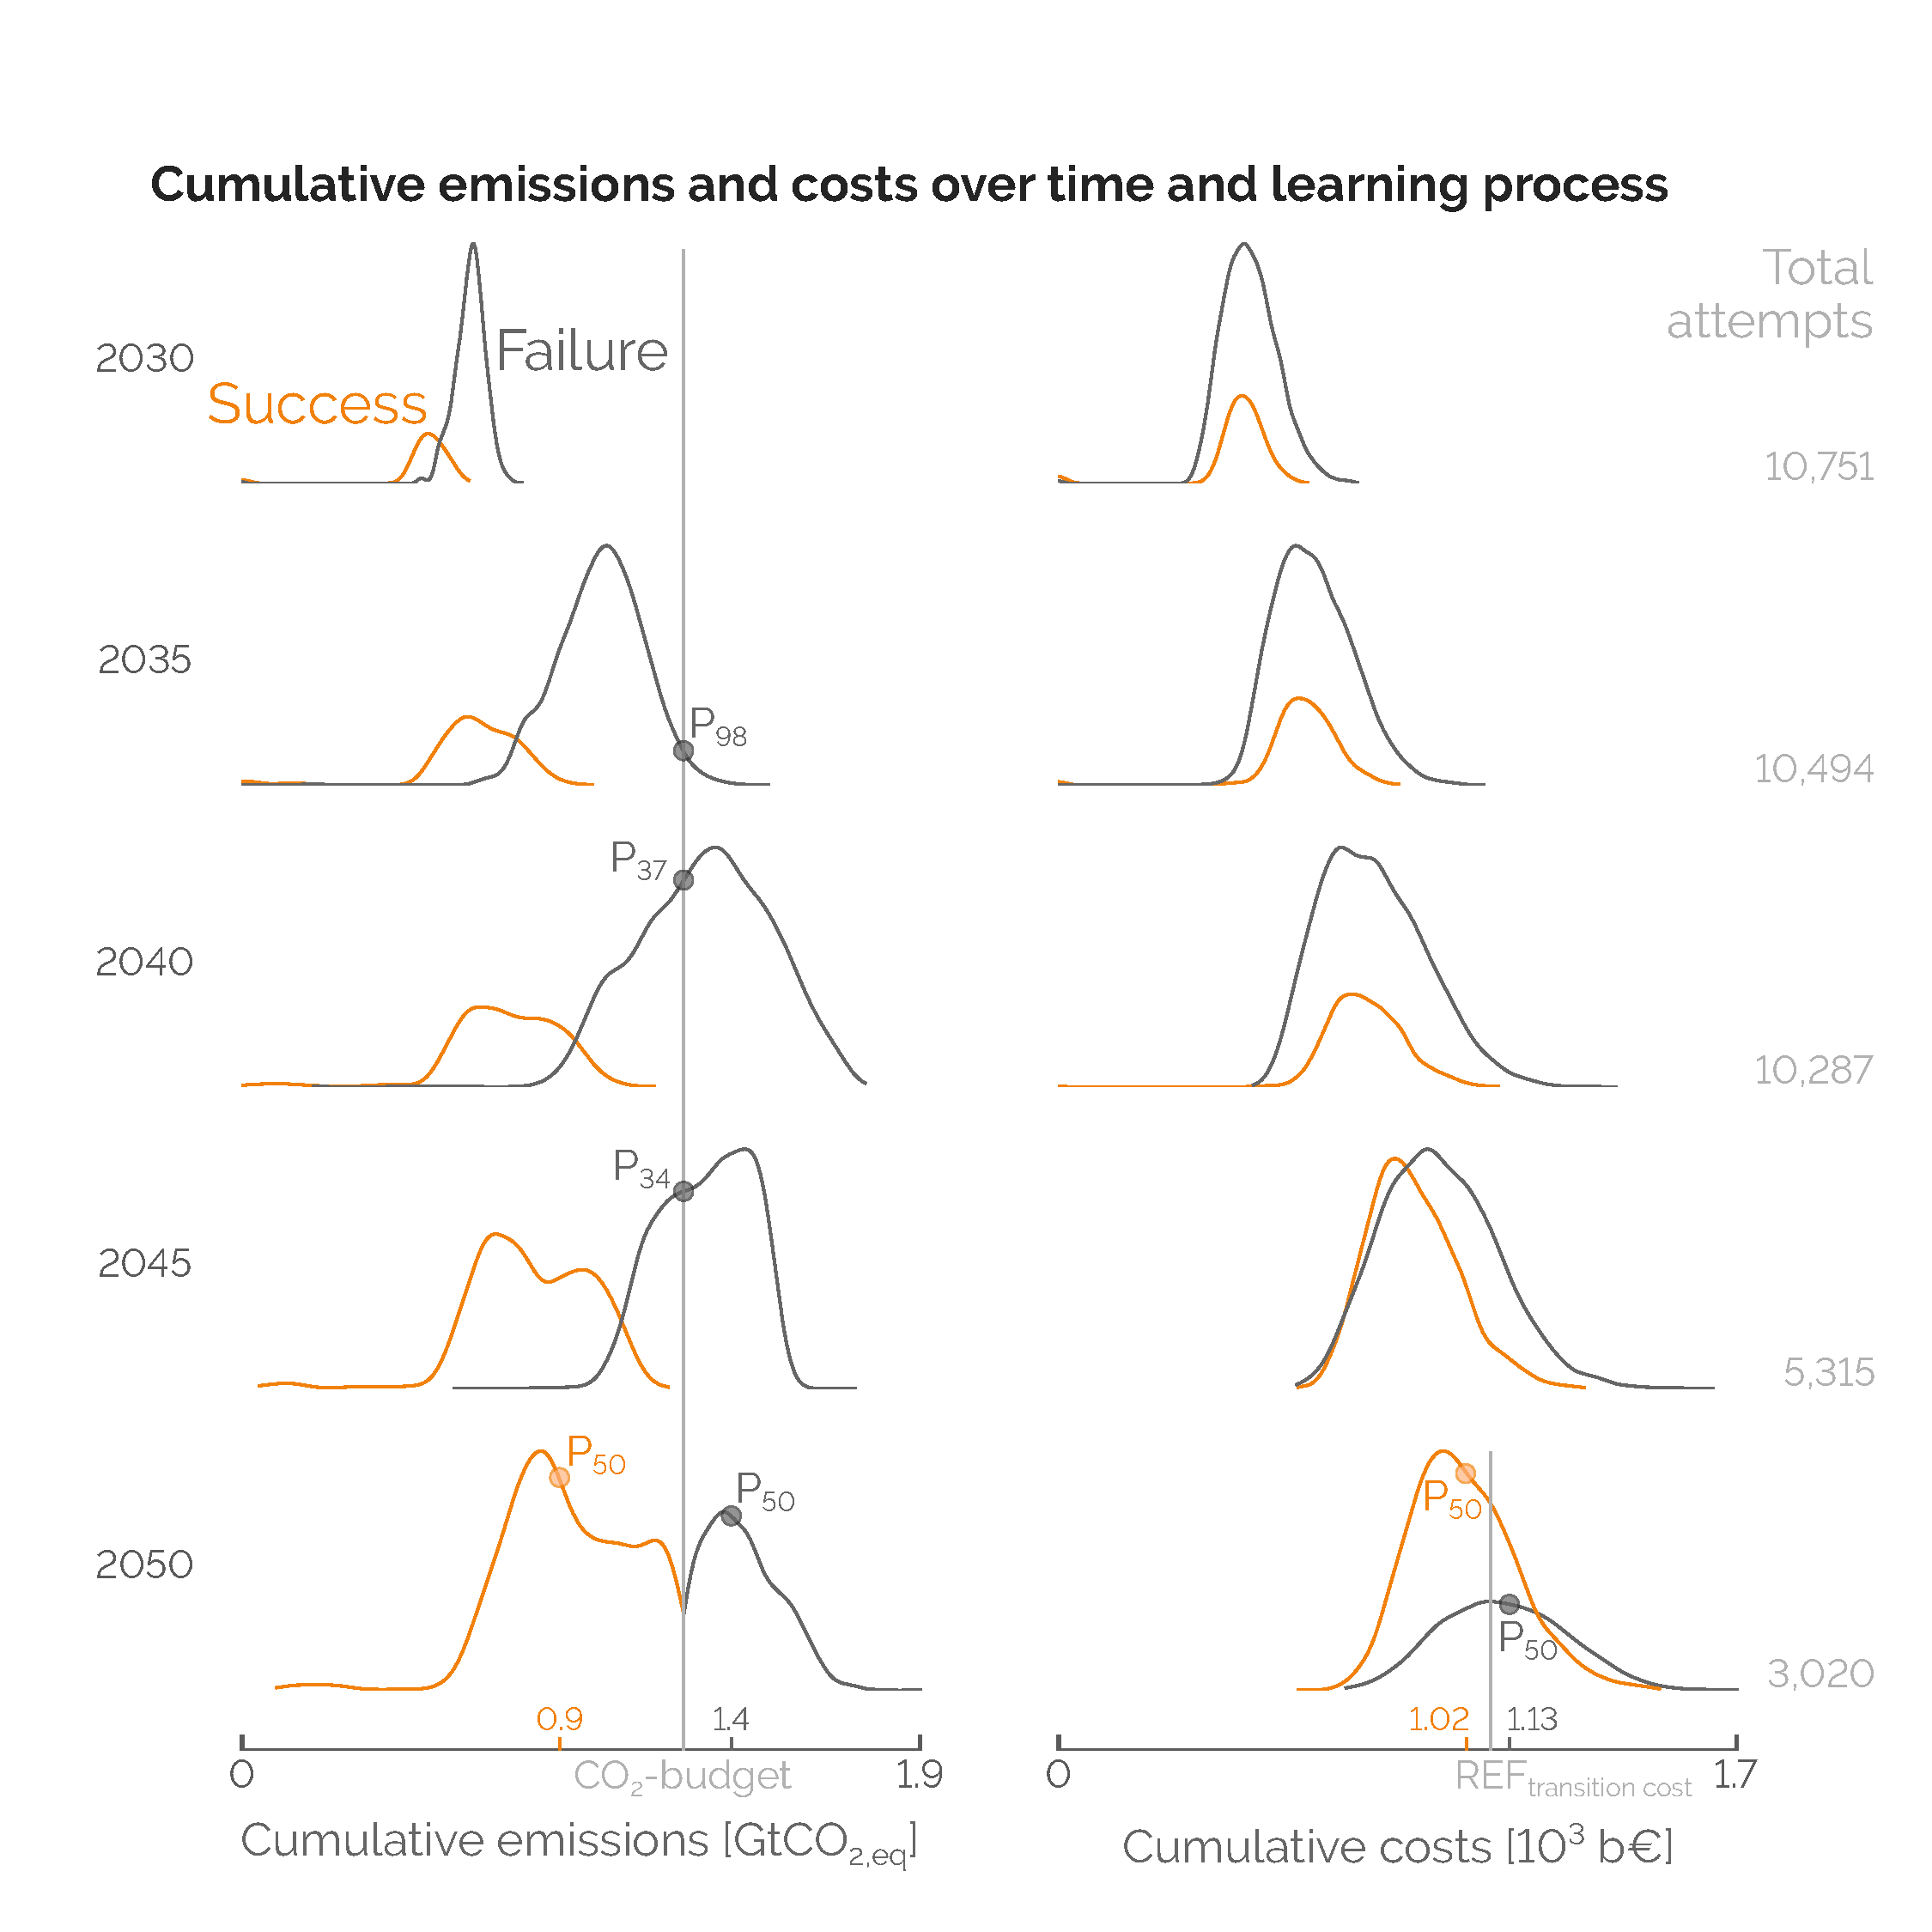
\includegraphics[width=0.8\textwidth]{Cum_gwp_cost_3.pdf}
\caption{Exploration of the state space over the learning process: cumulative emissions and costs. The majority of successful transitions have cumulative emissions much lower than the \ce{CO2}-budget and are cheaper than the REF case. }
\label{fig:Cum_gwp_cost}
\end{figure}

\newpage
Given the reward function (see Figure \ref{fig:Reward}), the agent optimises its policy by aiming at lowering the total transition cost as soon as it meets the \ce{CO2}-budget. The skewness of the cumulative emissions and costs in 2050 are indications of this reward function (see Table \ref{tab:skewness_gwp_cost}). When succeeding the transitions, the cumulative emissions have a negative skewness: the agent successfully stayed within the budget and most of the cases where close to that budget (median at 0.9 Gt$_{\ce{CO2},\text{eq}}$). On the contrary, the cumulative cost of successful transitions has a positive skewness: the agent successfully reduces the cost of the system as a secondary objective with 30\% of the cases above the reference transition cost. This hierarchy of agent's objective is verified with the failures. When it failed the transition, the agent aimed at reducing the emissions (skewness of 0.61) before minimising the total transition cost (skewness of 0.24). 

\begin{table}[htbp!]
\caption{Skewness of cumulative emissions and costs in 2050. Cumulative emissions are skewed to the left and to the right for the successes and failures, respectively. The skewness of the cumulative costs for successful transitions is higher compared to failures. On top of being the results of the optimisation through EnergyScope, these are influenced by the agent's policy that aims only at lowering the total transition cost as soon as it meets the \ce{CO2}-budget.}
\label{tab:skewness_gwp_cost}
\centering
\begin{tabular}{l c c}
\toprule
\textbf{Status of episode}  & \textbf{Skewness of cumulative} & \textbf{Skewness of cumulative} \\
\textbf{in 2050}  & \textbf{emissions} & \textbf{costs} \\	
\midrule
Success & -0.52 & 0.50 \\
Failure & 0.61 & 0.24 \\
\bottomrule							

\end{tabular}
\end{table}

\newpage
Finally, we observe that the majority of the successful transitions are cheaper than the reference transition cost, 1.1\,b€. Among the parameters impacting the most the total transition cost, we observe that success occurs when, on average,  the cost of purchasing fossil fuels is increased more than the one of electrofuels (see Table \ref{tab:param_RL}). In other words, to have higher chances to succeed a myopic transition, the key factor is to reduce the uncertainty on the cost of purchasing electrofuels or to increase the cost of fossil fuels. Given the skewness that is positive and negative for the electrofuels and the fossil fuels, respectively, these cases represent more than the majority of the successful cases. On top of this, total transition costs of successful episodes are lower due to lower industrial \gls{EUD} and discount rate. These favourable conditions combined with the right agent's actions led to transitions respecting the \ce{CO2}-budget.

\begin{table}[htbp!]
\caption{Uncertain parameters impacting the most the total transition cost, their Sobol' index and, for the successful transitions, their mean of their values between 0 and 100\%, $\mu$, and their skewness, $\gamma$. On top of being supported by the agent's actions, successful transitions occur when the cost of purchasing fossil fuels is more increased than the one of electrofuels.}
\label{tab:param_RL}
\centering
\begin{tabular}{l c c c}
\toprule
\textbf{Parameter}  & \textbf{$\mu$} & \textbf{$\gamma$}  \\	
\midrule
Purchase electrofuels & 50.4\% & 0.004  \\
Industry EUD & 49.8\% & 0.026 \\
Discount rate & 48.4\% & 0.089\\
Purchase fossil fuels  & 55.0\% & -0.068\\
\bottomrule							

\end{tabular}
\end{table}

Besides the cumulative emissions and costs, the agent also observes the share of renewable energy carriers in the primary mix and the efficiency of the system The share of renewable energy carriers in the primary mix allows identifying intermediate milestones along successful transitions (see Figure \ref{fig:RE_in_mix_Efficiency}). From the initial state of 10\% in 2020, a boost of integration of renewables in the near-term is needed to hope for a successful transition. For the successful occurrences to exceed failures, this share increases to 54\% in 2025. Along the transitions, this increase goes with the import of electrofuels and the full deployment of local \gls{VRES}. In 2050, the threshold where occurences of success are more numerous than failures was at 82\% of renewable share. In the REF case of Chapter \ref{chap:atom_mol}, this share reached 86\% by 2050. However, by 2050, Figure \ref{fig:RE_in_mix_Efficiency} shows another ``bump'' at lower share of renewables in the mix. This area corresponds to the possibility to install \gls{SMR}. As uranium is considered as a non-renewable resource \cite{rixhon2021terminology}, installing \gls{SMR} allows lowering the threshold as in the SMR case of Chapter \ref{chap:atom_mol}. Besides these milestones to respect the \ce{CO2}-budget of the transition, one can also look at the other side of the thresholds. Below the near-term threshold of $\sim$60\%, this is the ``no-go zone'' where succeeding the transition becomes unlikely, except if betting on the future installation of \gls{SMR}.

The efficiency, as defined in Section \ref{sec:RL:act_states_rew}, gives less valuable information towards successful transitions. Through the transition, besides the share of success increasing over the failures, the distributions of success and failure indistinguishably spread over the whole range. Similarly than the emissions, we observe a bump at lower efficiencies by 2050 due to the installation of \gls{SMR}.

\begin{figure}[!htbp]
\centering
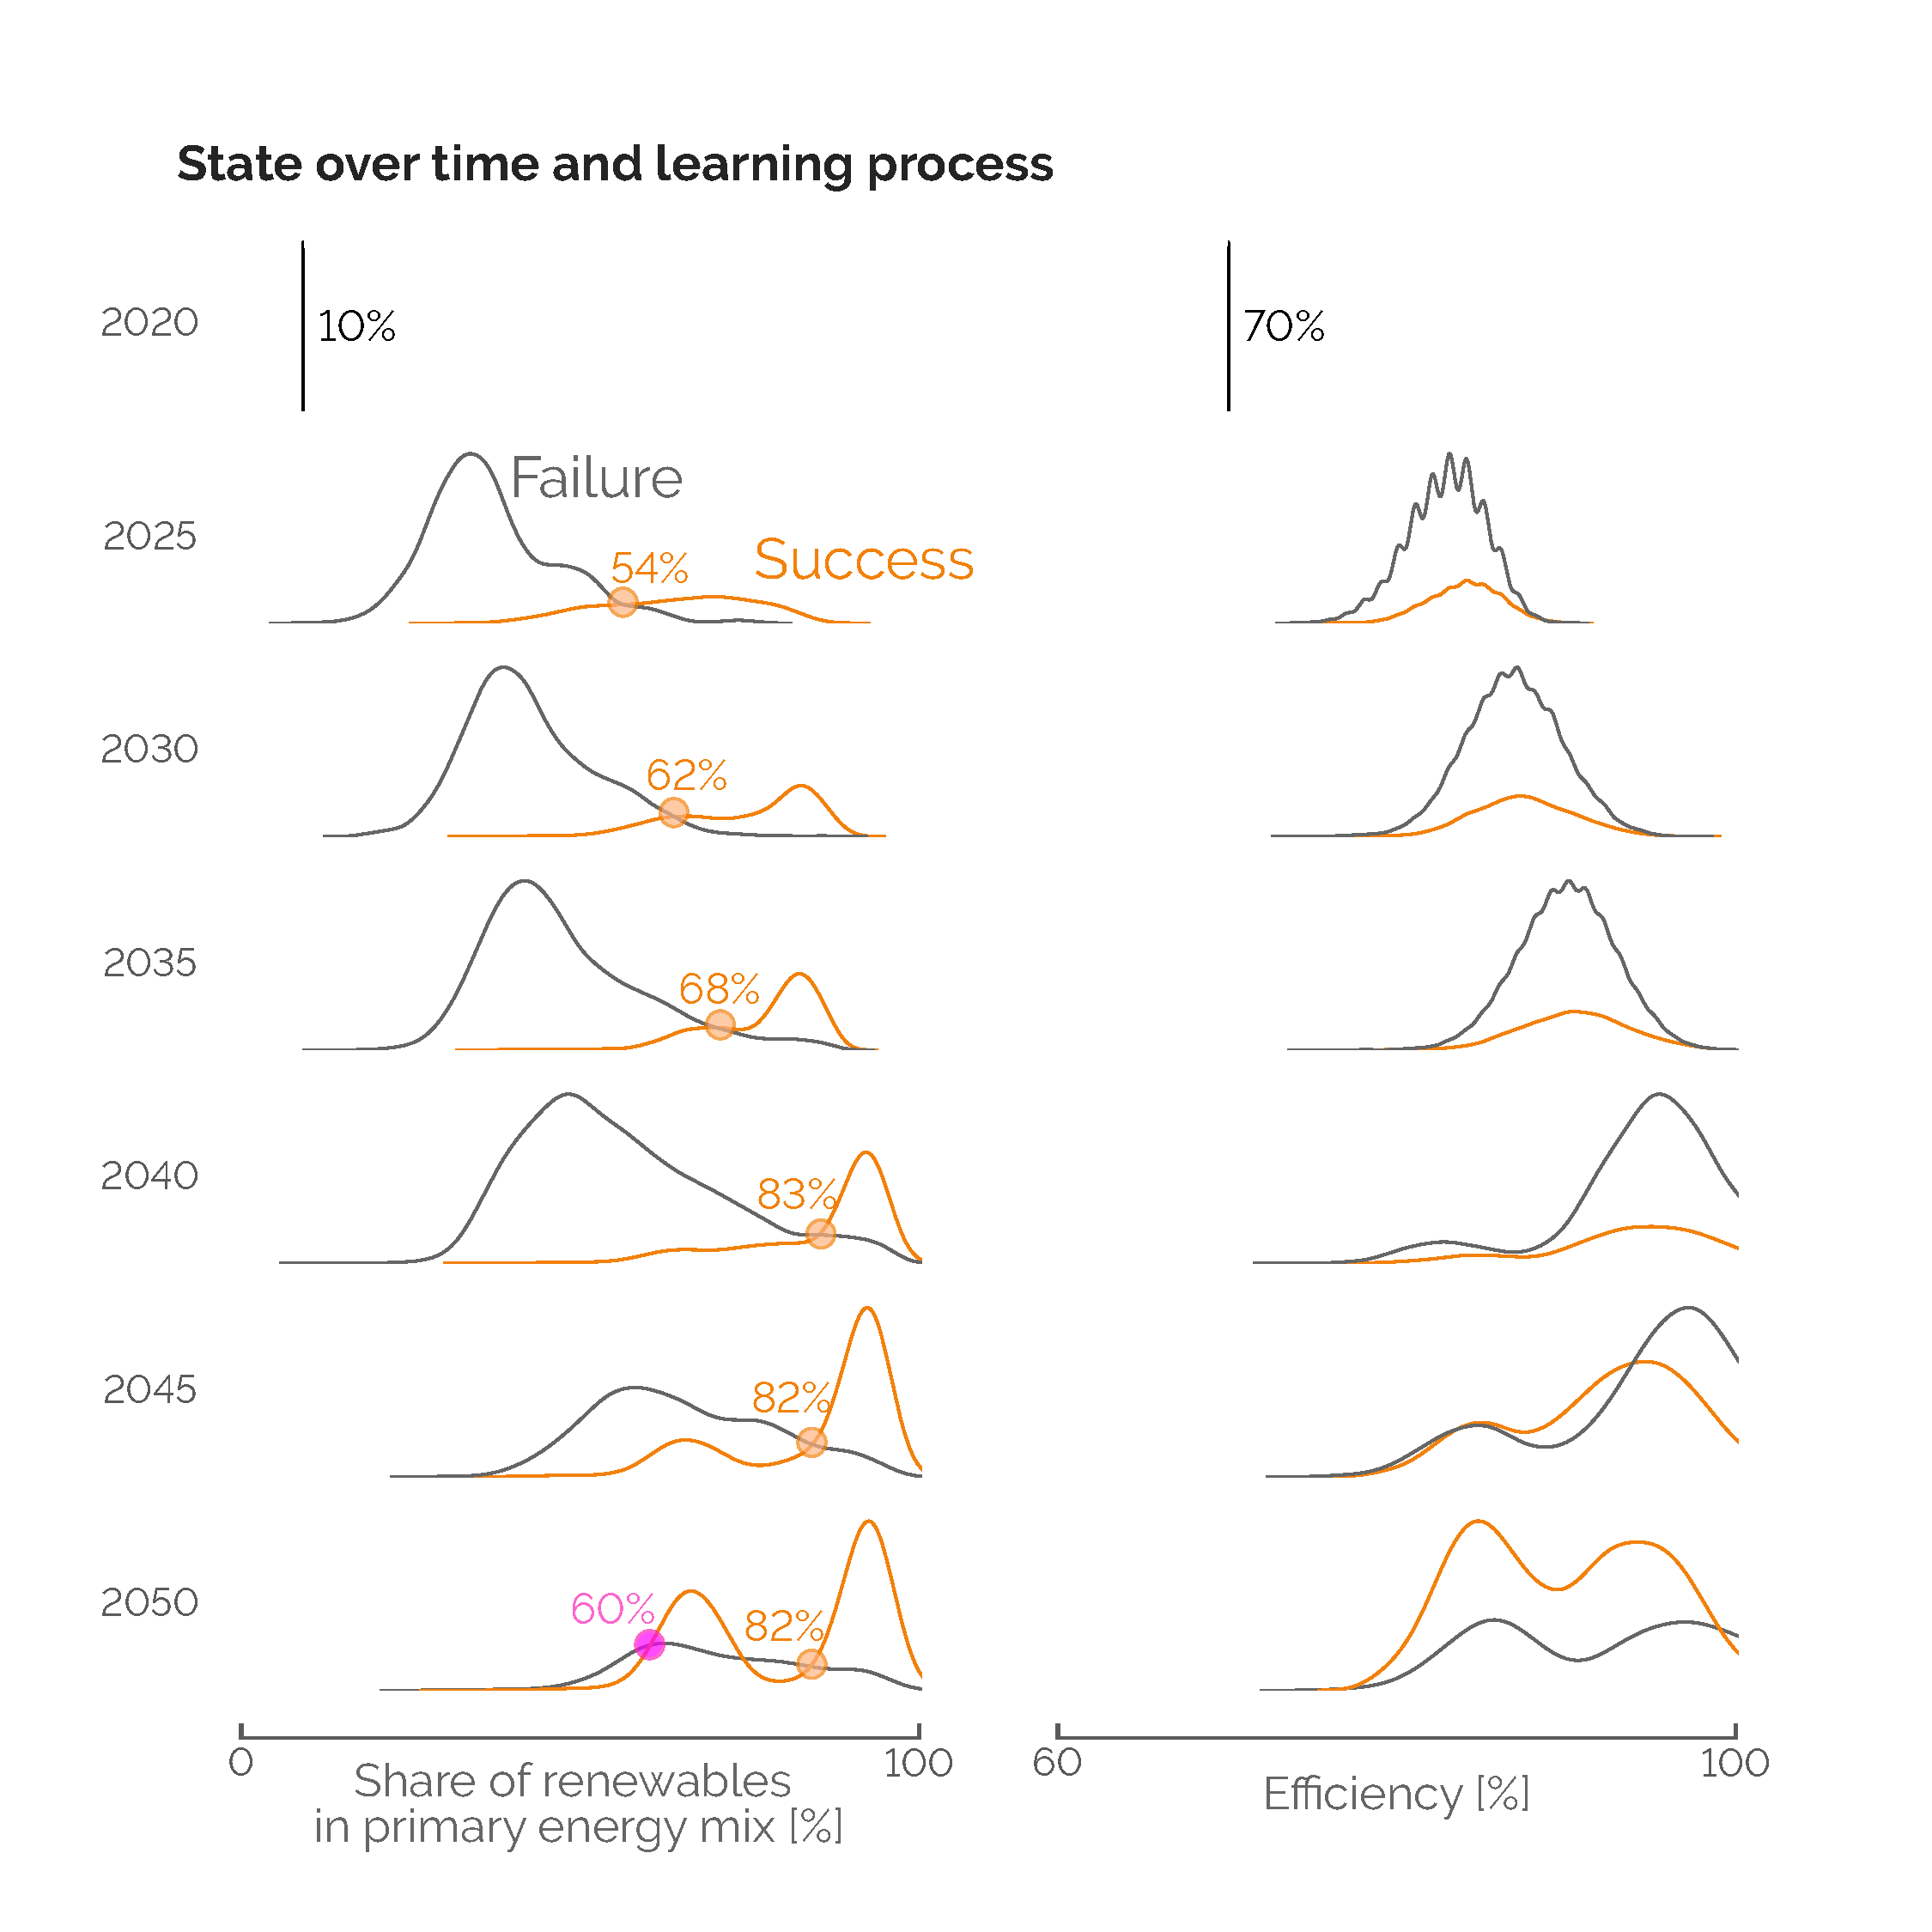
\includegraphics[width=0.8\textwidth]{RE_in_mix_Efficiency.pdf}
\caption{Exploration of the state space over the learning process: share of renewable energy carriers in the primary energy mix and efficiency. Integration of local \gls{VRES} at early stages then massive import of electrofuels later are needed to secure successful transitions. Below a near-term threshold ($\sim$60\%), the chances of success are limited, \ie no-go zones. Efficiency is a less valuable information for the agent to succeed transitions as failures and successes indistinguishably spread over the whole range.}
\label{fig:RE_in_mix_Efficiency}
\end{figure}

\subsection{Actions}
\label{subsec:RL:learning:actions}

After investigating the intermediate milestones to meet the \ce{CO2}-budget by 2050, this section details the actions the agent has taken during the learning process (see Figure \ref{fig:Actions_learning}). Rows represent the beginning of the time window at which the set of actions is taken. Similarly to the state space, we observe a wide exploration of the action space. The more the agent was able to progress through transition, without exceeding the \ce{CO2}-budget, the bigger is the share of successes compared to failures. Besides this observation, no specific range of values for the different actions at the different timing seems to lead to more successes. Looking at action individually, there does not seem to be any that supports more effectively the transition. The success come from the combination of these actions.

\begin{figure}[!htbp]
\centering
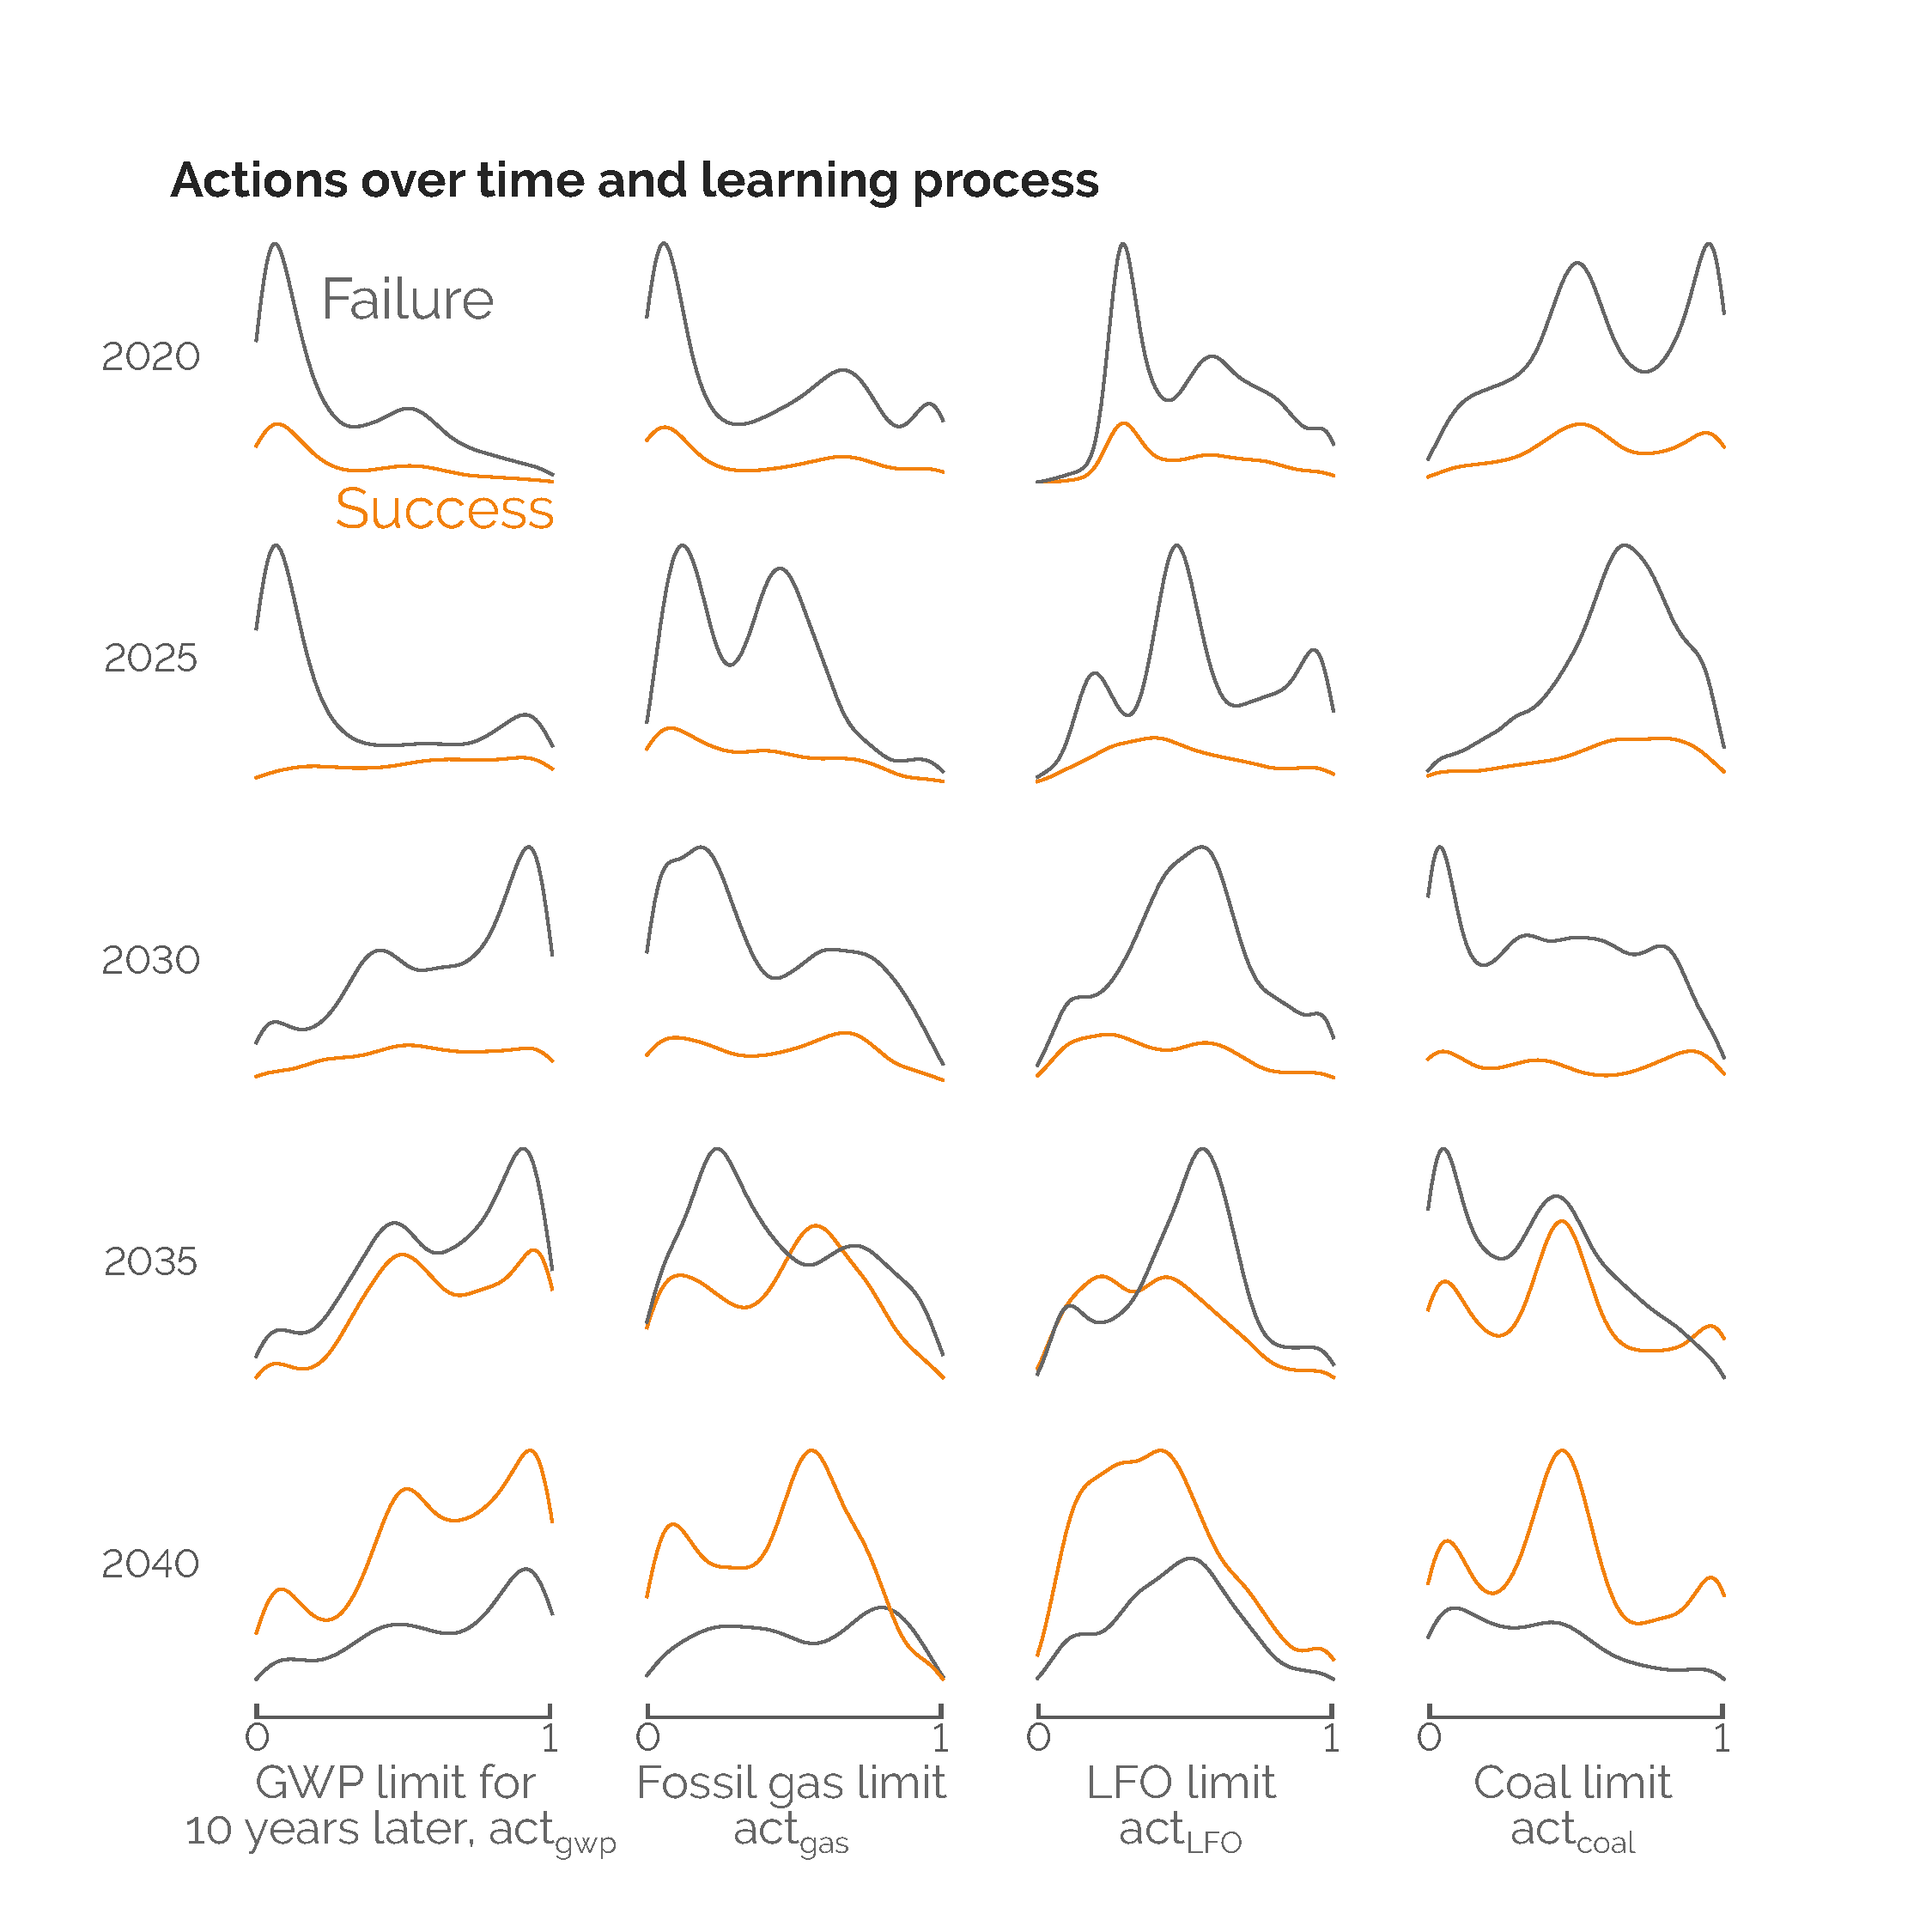
\includegraphics[width=0.8\textwidth]{Actions_learning.pdf}
\caption{Besides the wide exploration of the action space, successes and failures indistinguishably spread over the whole ranges of actions. In other words, it does not seem to be any clear set of actions to support successful transitions.}
\label{fig:Actions_learning}
\end{figure}

To identify the actions that have an actual impact on the environment, we can check if they are binding or not. In a \gls{LP} problem, constraints represent hyperplanes in the domain of variables. In a two-dimension space, these are straight lines (see Figure \ref{fig:Binding_constr}). When the problem is bounded and feasible, these lines are the edges of a convex polygon: the domain of feasibility. The optimal solution, $\textbf{x}^*$, is the combination of variables leading to the optimal value of the objective function. Besides being within the domain of feasibility, it is proven that this optimal solution, when unique\footnote{There are cases where the objective function has the same optimal value along an entire edge. In this case, there is an infinity of solutions and the problem is indeterminate.}, locates on a vertex of the domain \cite{bertsimas1997introduction}. The constraints intersecting at this vertex are considered as binding, actually limiting the objective function to be more optimal. In other words, binding constraints, when tightened, aggravate the objective value function. If these are inequality constraints, as represented in Figure \ref{fig:Binding_constr}, it means that their left and right sides of the equation are equal.

\begin{figure}[!htbp]
\centering
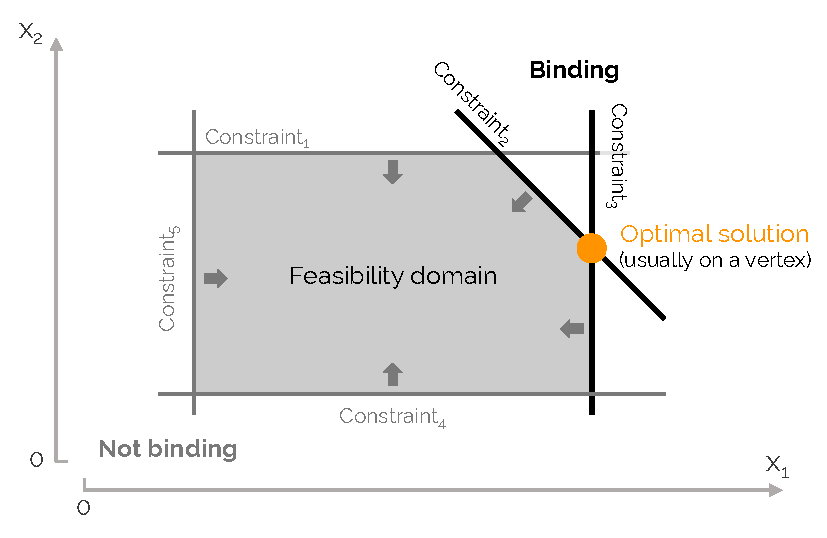
\includegraphics[width=0.7\textwidth]{Binding_constr.pdf}
\caption{Binding versus non-binding constraints. In \gls{LP} where the feasibility domain is non-empty and bounded, the constraints defined a convex feasibility domain in the space of variables (here, x$_1$ and x$_2$). The optimal solution usually locates on a vertex of this domain, \ie the intersection of several constraints (here, constraints 2 and 3) limiting the solution. These constraints are considered as binding, \ie having a limiting impact on the optimal solution.}
\label{fig:Binding_constr}
\end{figure} 

After filtering out failures of the learning episodes and keeping only the successful transitions, only a limited set of the actions are binding and have an actual impact on the result of the optimisation in EnergyScope Pathway (see Figure \ref{fig:Binding_learning}). This allows identifying key actions to support the myopic transition. Limiting the \gls{GWP} in the near-term is a key-factor for success. However, this action has a binding effect on the environment only at the end of the transition. The range over which limiting the use of fossil gas binds the optimisation is wider. Compared to other non-renewable fuels, this is due to the longer use of this energy carrier favoured by its low \gls{GWP} (the second after uranium) and its versatility (applications in the electricity, heat and mobility sectors).

\begin{figure}[!htbp]
\centering
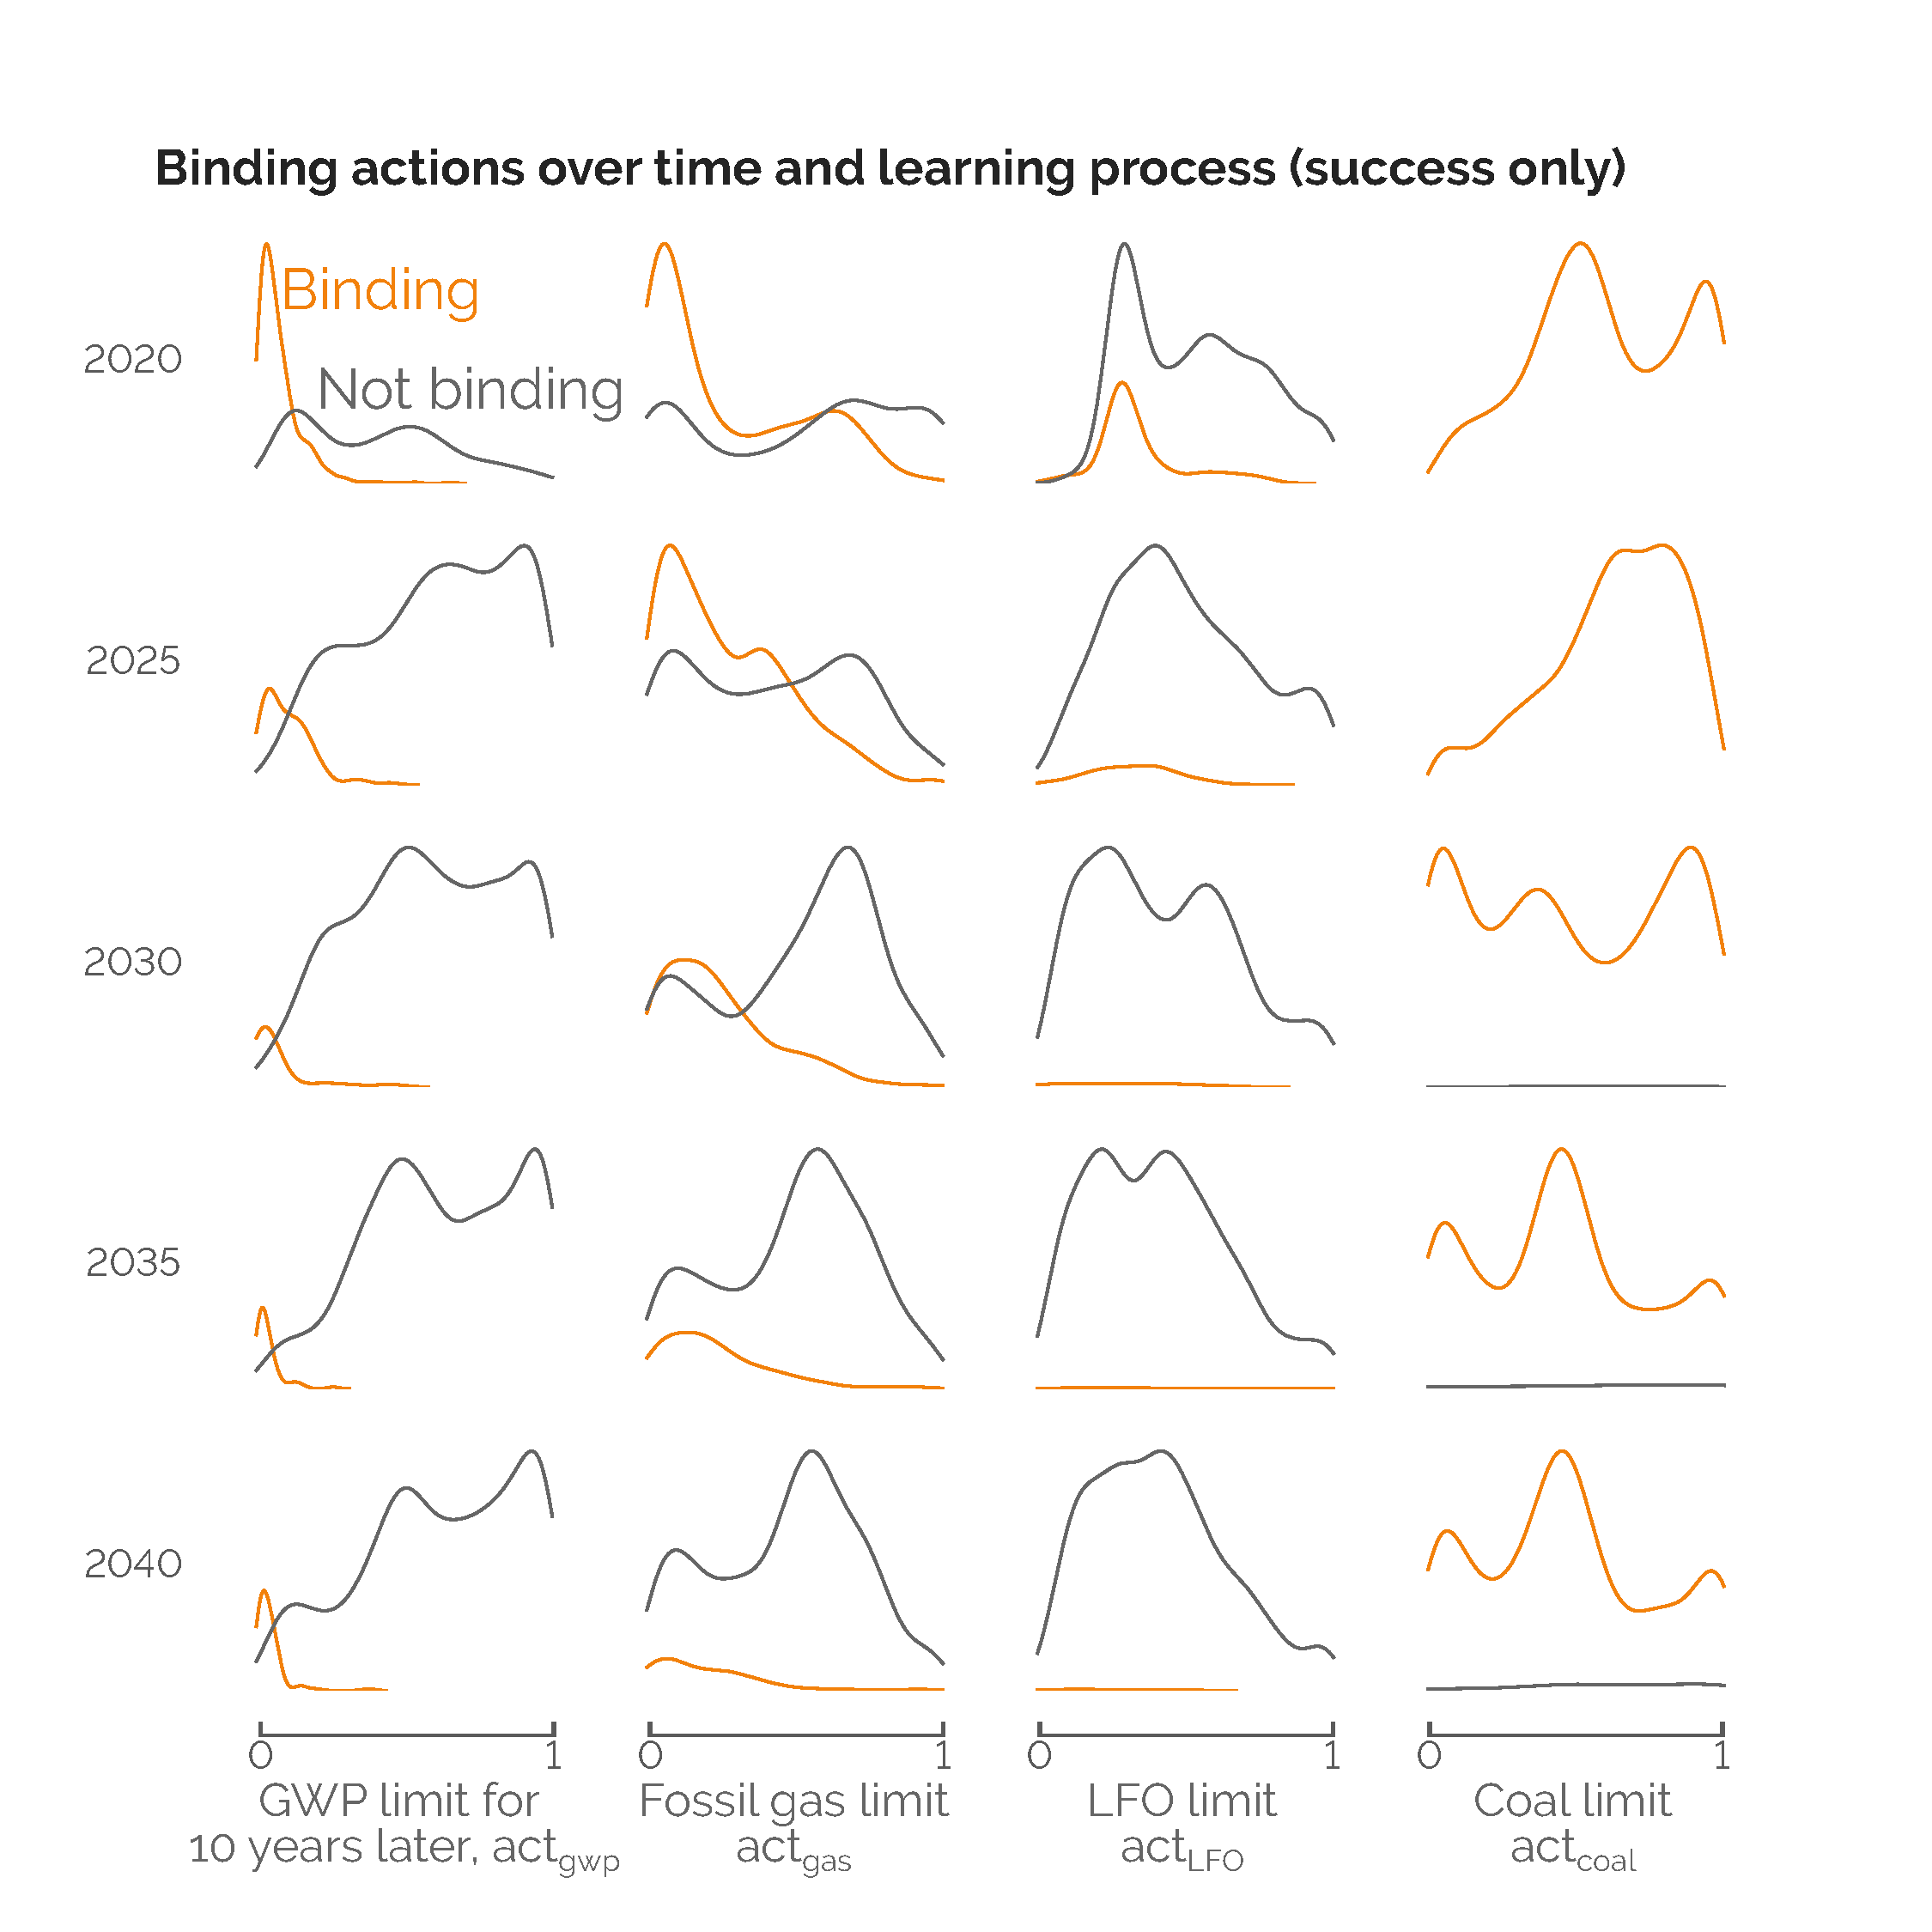
\includegraphics[width=0.8\textwidth]{Binding_learning.pdf}
\caption{Depending on the action and its timing, it is actually constraining the optimisation through EnergyScope Pathway or not. Sweet spots can be identified when considering the limits of \gls{GWP} and fossil gas consumption. Limiting coal consumption is always constraining, unlike \gls{LFO} that is ``naturally'' substituted by EnergyScope Pathway in the near-term.}
\label{fig:Binding_learning}
\end{figure}

When it comes to limiting the use of \gls{LFO} and coal, the conclusions are more straightforward. At the beginning of the transition, most of the 159\,TWh of \gls{LFO} are consumed by naphtha-cracker (46\%) and decentralised boilers (45\%). The remaining 10\% are consumed by industrial boilers. Even though \gls{LFO} represents  30\% of the primary energy mix in 2020, the cost-optimum removes it of the mix without requiring the action of the agent. Naphtha-crackers, decentralised and industrial boilers get substituted by \gls{MTO}, decentralised \gls{HP} and industrial resistors and \gls{CHP}, respectively.  This ``non-bindness'' of limiting \gls{LFO} is an indication that this action could be removed from the agent's levers of action without impacting the optimisation of its policy.

On the contrary, limiting coal is always binding. Before all, this is due because coal is a cheap resource (17\,€/MWh). In other words, the cost-driven environment will favour it. Then, as the maximum amount of coal (28\,TWh) is much smaller than fossil gas and \gls{LFO}, high value of $\mathrm{act}\textsubscript{coal}$ still represents small consumption of coal.

\newpage
\section{Comparison with references}
\label{sec:RL:testing}
After investigating the exploration of myopic transition, this section compares these results with the perfect foresight under uncertainties from the \gls{UQ} analysis presented in Chapter \ref{chap:atom_mol}. To reduce the computational time, the monthly model could also be used to carry out \gls{RL}-based exploration of myopic pathways. Appendix \ref{app:app_RL_TD_MO} presents the comparison between the results obtained from the learning process on the hourly and monthly models.

\gls{RL}-based myopic optimisation provides \ce{CO2}-emissions pathways different from the perfect foresight approach to respect the same \ce{CO2}-budget (see Figure \ref{fig:Gwp_pathway}). However, driven first by this \ce{CO2}-budget, the agent often reaches much lower cumulative emissions when succeeding the transition (see Figure \ref{fig:Cum_gwp_cost}). This comes from the agent's actions that limit the emissions and/or the consumption of fossil resources at the early stages. Thanks to the bigger reduction of emissions at these early stages, the \gls{RL}-based optimisation can benefit from a ``\ce{CO2}-buffer'' at the end of the transition. This buffer is compensated by the end of the transition where 50\% of the myopic transitions reach 2050 with 10 or more remaining Mt$_{\ce{CO2},\text{eq}}$ compared to 4 for the perfect foresight approach. These remaining emissions by 2050 come from the consumption in industrial boilers of waste and coal that account for 3.5\% and 2.4\% on average by 2050. Finally, the long-term vision of the perfect foresight approach results in smoother reduction of the emissions to end up with less emissions by 2050.

The comparison between the failures and the pathways demonstrates the added-value brought by myopic pathway optimisation. In the near-term (2025-2030), levels of emission are similar between perfect foresight and myopic cases that have failed. This shows that limited foresight encourages to strongly act at the early stages. On top of this, following the initial steps of \ce{CO2}-emissions pathways resulting from PF approach would likely ($\sim$80\%) lead to fail the transition. 

\begin{figure}[!htbp]
\centering
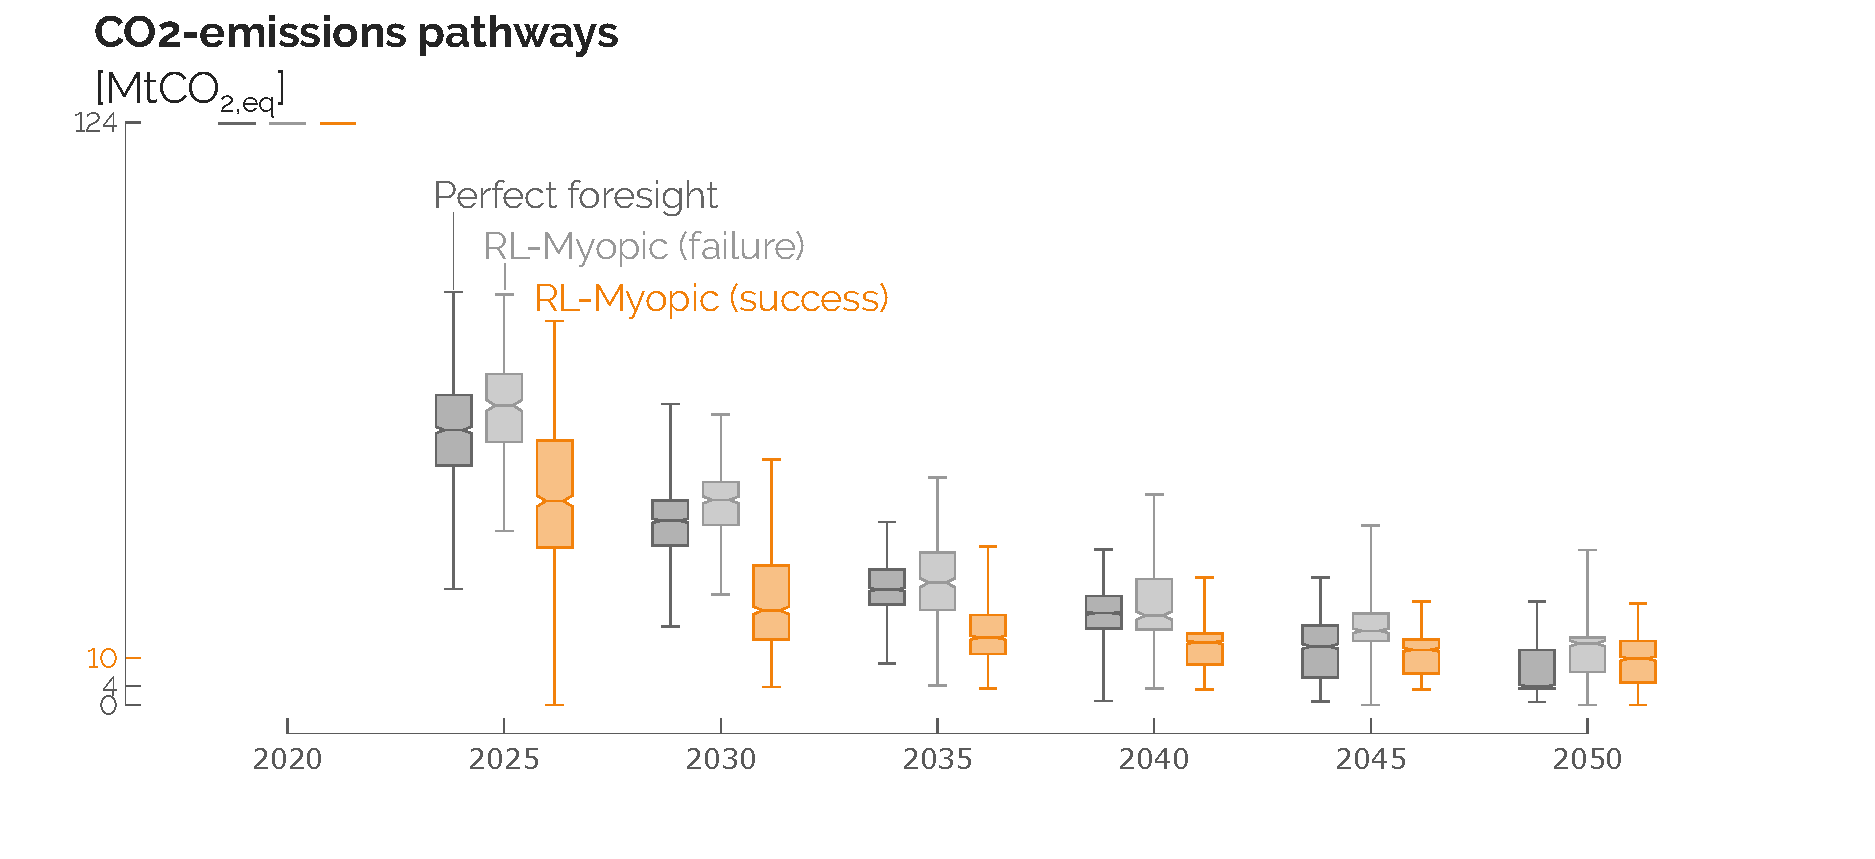
\includegraphics[width=0.8\textwidth]{Gwp_pathway_core.pdf}
\caption{Comparison of \ce{CO2}-emissions pathways from the perfect foresight optimisation under uncertainties and the \gls{RL}-based myopic optimisation. }
\label{fig:Gwp_pathway}
\end{figure}

The transition pathways of the annual system cost show another impact of the agent in the \gls{RL}-based exploration (see Figure \ref{fig:System_cost_pathway}). Via its actions and its cost-based reward, the agent can reach systems that are cheaper than any other solution obtained by the perfect foresight approach. The perfect foresight approach gives a wider variability in its cost since this method always found a solution even in worst conditions such as high cost of purchasing resources and high \gls{EUD}. 

\begin{figure}[!htbp]
\centering
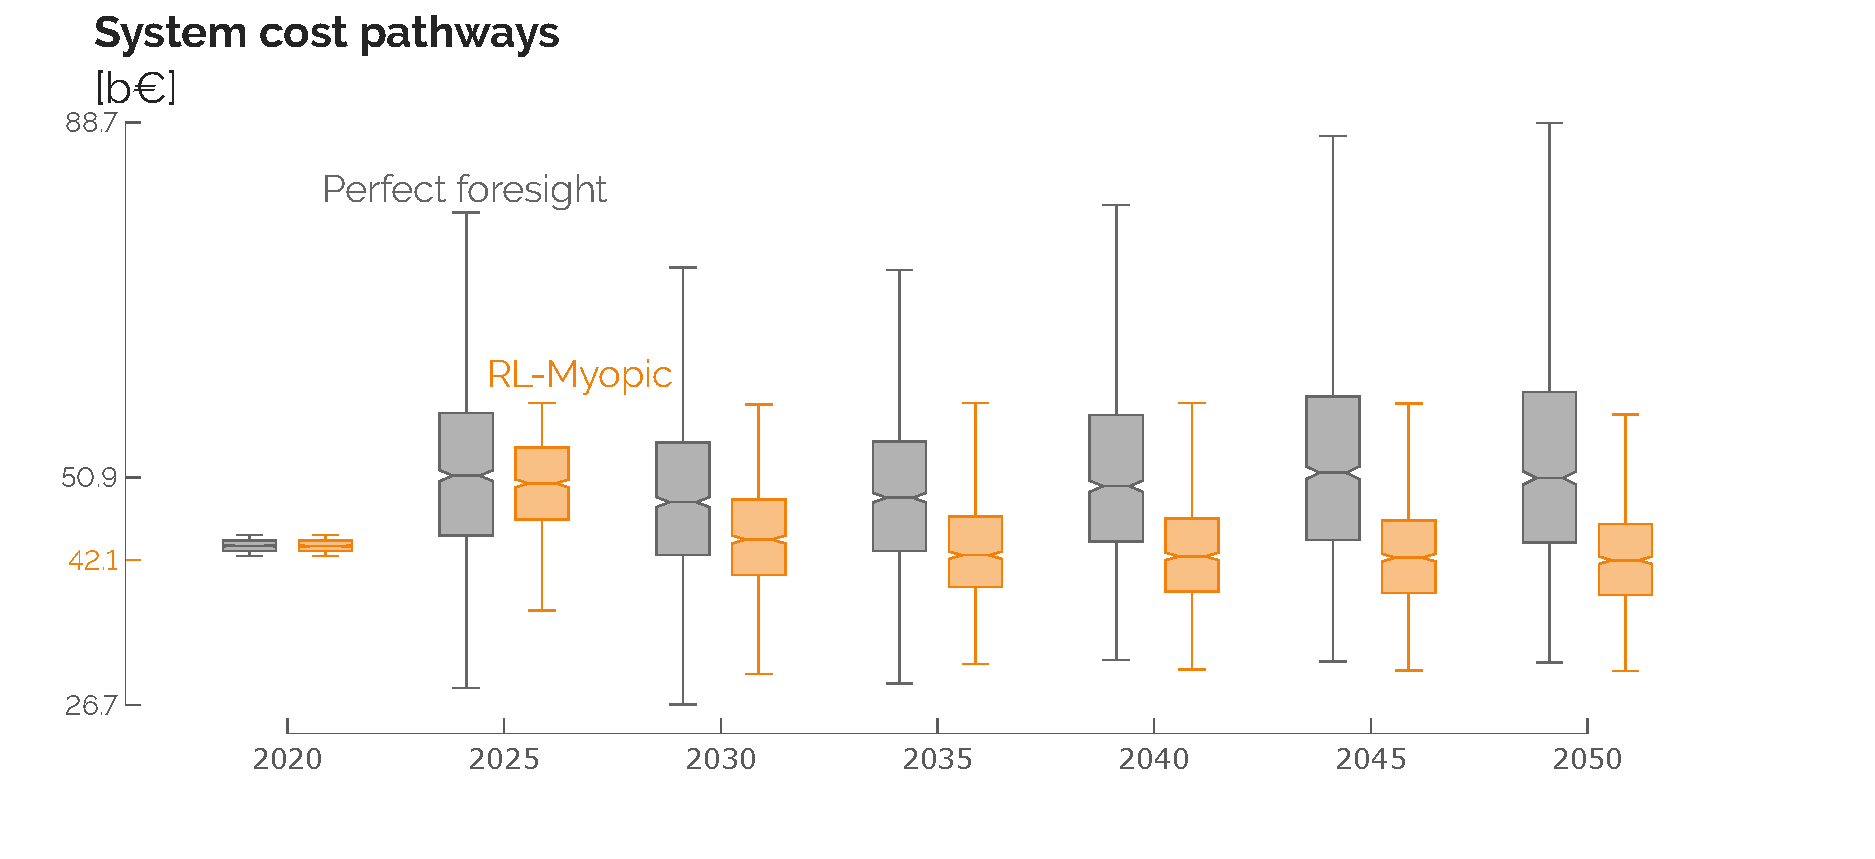
\includegraphics[width=0.8\textwidth]{System_cost_pathway_core.pdf}
\caption{Comparison of annual system costs pathways from the perfect foresight optimisation under uncertainties and the \gls{RL}-based myopic optimisation.}
\label{fig:System_cost_pathway}
\end{figure}

\newpage
The analysis of the cumulative costs shows that the \gls{OPEX} is the main difference between myopic and perfect foresight transitions (see Figure \ref{fig:Opex_Capex_Salvage_comp}). Supported by the agent's actions, successful myopic transitions have a lower \gls{OPEX} than the perfect foresight ones.

\begin{figure}[!htbp]
\centering
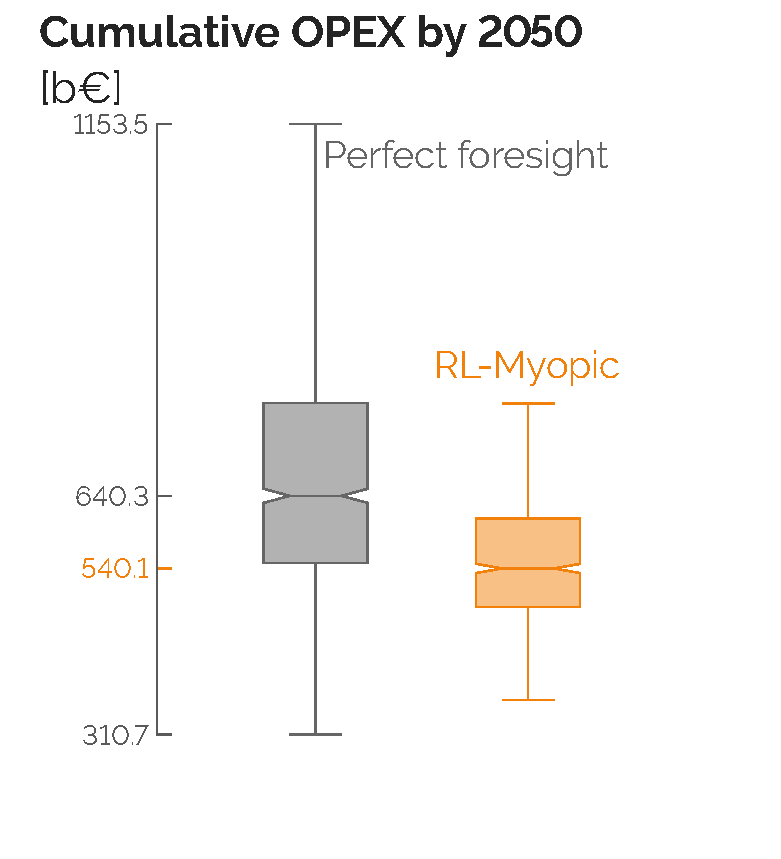
\includegraphics[width=0.325\textwidth]{Opex_2050_comp_core.pdf}
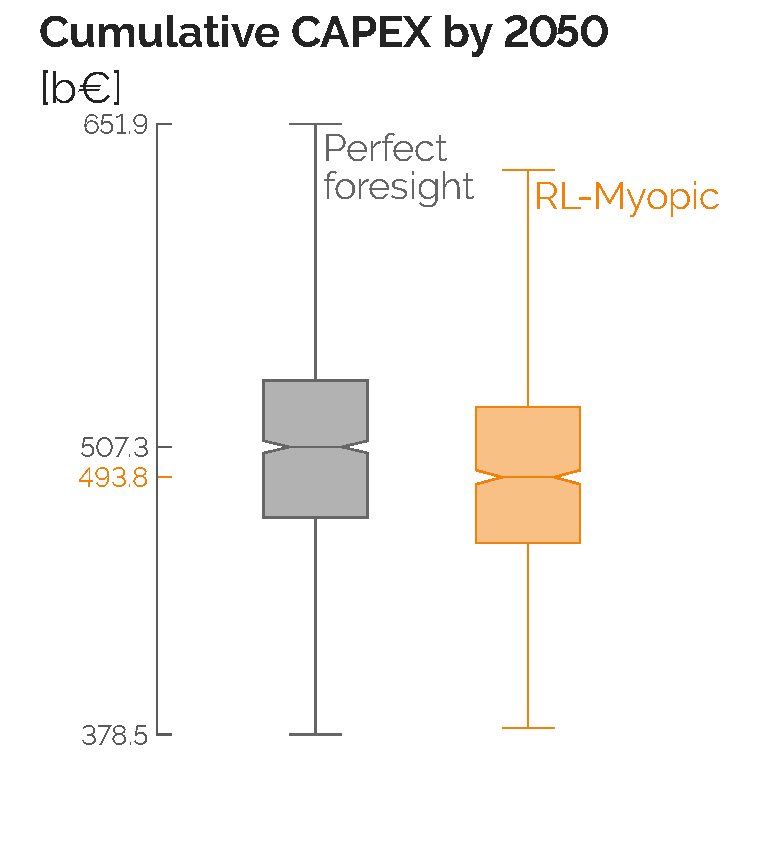
\includegraphics[width=0.325\textwidth]{Capex_2050_comp_core.pdf}
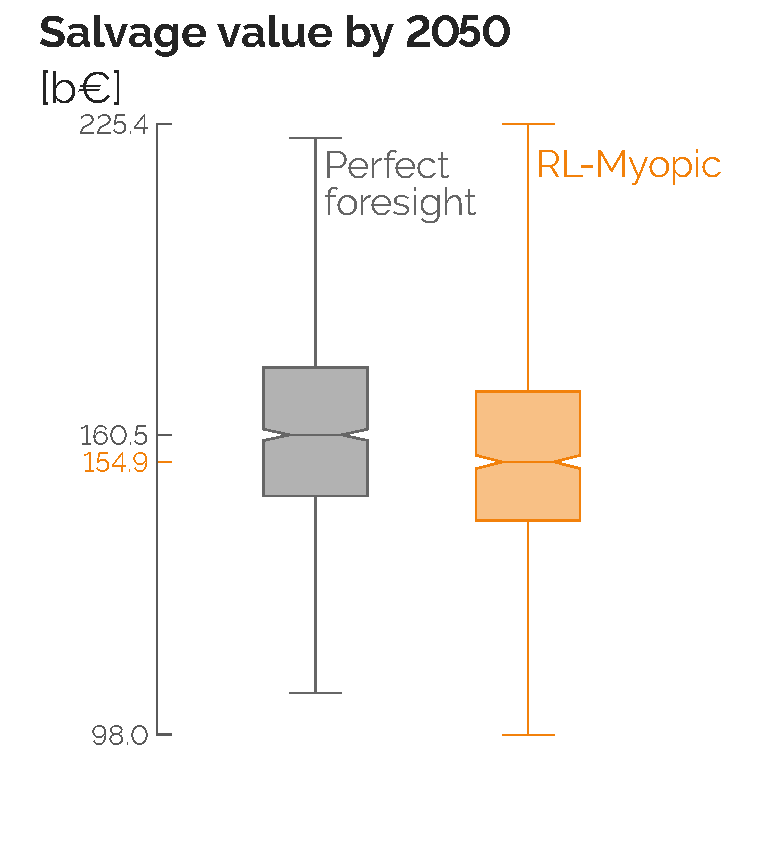
\includegraphics[width=0.325\textwidth]{Salvage_2050_comp_core.pdf}
\caption{Comparison of cumulative OPEX (left), CAPEX (center) and salvage value (right) in 2050 from the perfect foresight optimisation under uncertainties and the \gls{RL}-based myopic optimisation.}
\label{fig:Opex_Capex_Salvage_comp}
\end{figure}

The cost of purchasing the energy carriers represents about 70\% of the total cumulative \gls{OPEX}. The assessment of the primary energy mix by 2050 highlights that the difference of OPEX between the perfect foresight and the myopic pathways come from the import of electrofuels, and especially of e-ammonia (see Figure \ref{fig:Mix_2050_comp}).  In the majority of the cases, e-ammonia is more than two times more imported in the myopic transitions. Being cheaper than e-methane (see Chapter \ref{chap:case_study}), e-ammonia brings flexibility in the production of electricity via \gls{CCGT} (see Chapter \ref{chap:atom_mol}). Besides the slightly favourable economical conditions (see Table \ref{tab:param_RL}), the myopic optimisations opt to invest massively into importing renewable molecules because of the limited knowledge in the future, and, among others, the availability of \gls{SMR}. This explains why 50\% of the successful transitions reached cumulative emissions below 900\,Mt$_{\ce{CO2},\text{eq}}$ (see Figure \ref{fig:Cum_gwp_cost}).

\begin{figure}[!htbp]
\centering
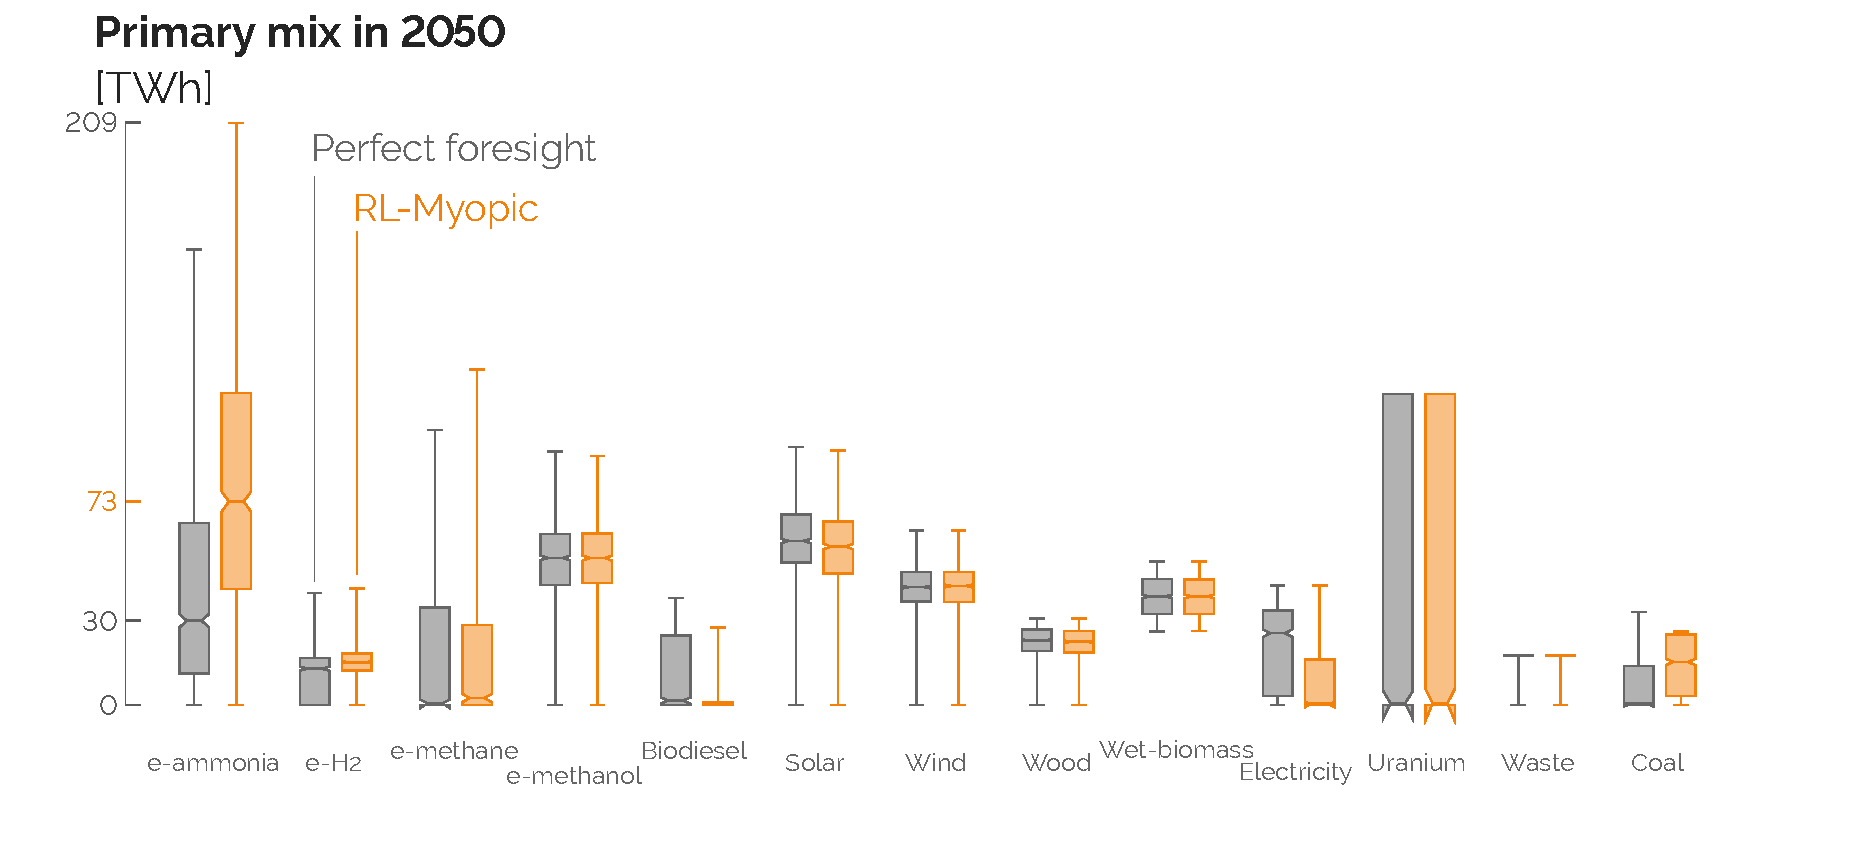
\includegraphics[width=0.8\textwidth]{Mix_2050_comp_core.pdf}
\caption{Comparison of the primary energy mix in 2050 from the perfect foresight optimisation under uncertainties and the \gls{RL}-based myopic optimisation. The biggest difference is about e-ammonia to supply \gls{CCGT}.}
\label{fig:Mix_2050_comp}
\end{figure}


\section{Conclusions}
\label{sec:RL:conclusions}
In the literature, two options are investigated to explore transition pathways of a whole-energy system: perfect foresight and myopic. In perfect foresight optimisation, a full knowledge of the parameters is assumed over the entire time horizon. To add more realism, myopic optimisation considers a sequence of more limited time windows leading to the end of the time horizon \cite{poncelet2016myopic}. To respect a \ce{CO2}-budget over the transition, this case requires a prescribed \ce{CO2}-trajectory \cite{fais2016impact}. However, since the effect of \ce{CO2}-emissions in climate change is cumulative, the total amount of these emissions matters more than the trajectory itself. Consequently, we have applied the \acrfull{RL} approach on the environment of the Belgian myopic pathway optimisation under uncertainties.

%In the \gls{RL} framework, the agent had four actions to support the 2020-2050 transition: (i) limiting the \ce{CO2}-emissions at the end of each successive time window and limiting the consumption of (ii) fossil gas, (iii) \acrfull{LFO} and (iv) coal. The reward fed back by the environment to the agent focused first on meeting the \ce{CO2}-budget, 1.2\,Gt$_{\ce{CO2},\text{eq}}$ equivalent to 10 years at the current level of emissions. A secondary focus is also put on aiming at a minimum transition cost. To know its progress through the transition, the agent has the information of the cumulative emissions and costs as well the share of renewable energy carriers in the primary energy mix and the system overall efficiency.

This \gls{RL}-based exploration pointed out that short-term actions were needed to hope succeeding such a transition, as also demonstrated by \citet{luderer2018residual}. Where \gls{LFO} becomes less cost-competitive in the near-future, limiting the use of coal should be done at any cost. Then, fossil gas should be replaced by e-methane in the mid-term while putting a strict limit on the overall emissions becomes the most effective action by the end of the transition. The analysis of the share of renewables in the primary energy mix highlighted intermediate milestones to have higher chances to succeed the transition. Below 54\% of renewables in the mix in the near-future, these chances become much more limited, \ie the no-go zone. 

We have compared the results coming from this \gls{RL}-based myopic optimisation with the hourly perfect foresight approach. These myopic optimisations provided pathways respecting the \ce{CO2}-budget that were more drastic in cutting emissions in the short-term than the perfect. Supported by the agent's actions, we could reach cheaper energy system than what the perfect foresight could give. This comparative analysis also pointed out that investing more into renewable electrofuels was the option when knowledge about the future is limited. To do so, it requires reducing the uncertainties of their cost of purchasing. 

Further analyses should assess more accurately the impact of uncertainties on the agent's capacity to succeed the myopic transition. These analyses would aim at identifying the parameters that should necessarily be in specific ranges to allow the agent to succeed. On the contrary, there could be ranges of values for which the chances of success would be much more limited.

In conclusion, via the application of the \gls{RL} approach, we have widely explored the different myopic transition pathways and identified sweet-spots (and no-go zones) to succeed a transition with an ambitious \ce{CO2}-budget target. It also highlighted the actions to take to effectively support a whole-energy system transition.
%\clearpage

% -- Conclusion ----------------------------------------------------
%\clearemptydoublepage
%\chapter*[Conclusions]{Conclusions} 
%\addcontentsline{toc}{chapter}{Conclusions}
%%!TEX root = ../thesis_main.tex
%!TEX encoding = UTF-8 Unicode
I took here the same sections as in Gauthier's thesis
\section*{Thesis contributions}
\addcontentsline{toc}{section}{Thesis contributions}
Insist here on the methodological added value of the thesis

\section*{Limitations}
\addcontentsline{toc}{section}{Limitations}
\begin{itemize}
\item Due to the formulation of the salvage value, some technologies remain in place whereas they are not used anymore (see Appendix B.3, e.g. coal boilers and naphtha-cracker). It's better for the system to keep unused assets to recover part of their salvage value than prematurely decommissioning them.
\end{itemize}

\section*{Application outcomes}
\addcontentsline{toc}{section}{Application outcomes}
What this new methodology has brought over when applied to the case of Belgium

\section*{Recommendations and guidance}
\addcontentsline{toc}{section}{Recommendations and guidance}
What to do then for policymakers, how to use the tool

\section*{Perspectives}
\addcontentsline{toc}{section}{Perspectives}
List the future works to build upon the thesis

\begin{itemize}
\item \textbf{Word about sufficiency} oui mais c'est sans doute celle qui est le plus enviable car la moins risqué à tenter d'atteindre, les solutions mirages technologiques, si on y croit trop on met tout la dessus et si ca foire, on est encore plus dans la merde pcq la direction est mauvaise, la solution sobriété, meme si jamais atteint les efforts pr l'atteindre ne seront pas contre productif
\item \textbf{Word about availability of electrfuels} Voir mémoire Ced et Simon
\item Extract a roadmap representative of a multiple-run UQ or RL process.
\item In this work, we only consider emissions related to the use of energy carriers and not the construction
\end{itemize}


Quand je parle de ce que j'ai fait avec RL : Starting from the initial state of the energy system in 2020, the agent takes every five years a set of actions until reaching 2050. Although, these actions are taken every five years, they impact the system, for the next ten years --- their time window. The intermediate solutions obtained in the middle of the time window are used as a new starting point for the agent that makes a new series of decisions for the next ten years, etc. Repeating the whole transition with different sequences of actions-states allow the agent to come up with an optimised policy towards sustainability, considering the variation of the parameters of its environment.

%\clearpage

%\clearemptydoublepage

%%%%%%%%%%%%%%%%%%%%%%%%%%%%%%%%%%%%%%%%%%%%%%%%%%%%%%%%%%%%%%%%%%%%
%%                                                                %%
%%                        BIBLIOGRAPHY                            %%
%%                                                                %%
%%%%%%%%%%%%%%%%%%%%%%%%%%%%%%%%%%%%%%%%%%%%%%%%%%%%%%%%%%%%%%%%%%%%

%\backmatter

%\addcontentsline{toc}{chapter}{Bibliography}
\bibliography{/Users/xrixhon/Development/GitKraken/THESIS/bib_thesis.bib}

%\clearemptydoublepage


%%%%%%%%%%%%%%%%%%%%%%%%%%%%%%%%%%%%%%%%%%%%%%%%%%%%%%%%%%%%%%%%%%%%
%%                                                                %%
%%                        APPENDICES                              %%
%%                                                                %%
%%%%%%%%%%%%%%%%%%%%%%%%%%%%%%%%%%%%%%%%%%%%%%%%%%%%%%%%%%%%%%%%%%%%

\begin{appendices}

% -- Appendix 1 - Full results -------------------------------------
\chapter{Belgian energy system in 2020}
\label{app:bel_2020}
The Belgian whole-energy system of 2020 was largely based (88.6\% of the primary energy mix) on \og conventional fuels\fg (\ie oil and oil products (38.2\%), natural gas (29.5\%), uranium (16.3\%) and solid fossil fuels (4.6\%) while the rest mainly accounts for 26.7\,TWh of lignocellulosic and wet biomass, 12.8\,TWh of wind and 5.1\,TWh of solar \cite{spf_economy_2022}. Given the data available in the literature (mostly for the power sector) and, when not available, following the assumptions made by \citet{Limpens2020}, \Cref{tab:Belgium_2020} gives the major technologies used in 2020 to supply the different demands of \Cref{fig:cs_demands}.

\begin{table}[htbp!]
\caption{Major technologies used to supply the 2020-demands of \Cref{fig:cs_demands} in terms of share of production and installed capacity. $^{(a)}$ The decentralised heating units provide 98\% of the low-temperature heat demand. $^{(b)}$ The private mobility accounts for 80\% of the passengers mobility.}
\label{tab:Belgium_2020}
\begin{minipage}{\linewidth}
\centering
\resizebox{\textwidth}{!}{
\begin{tabular}{l c c c}
\toprule
\multirow{2}{*}{\textbf{End-use demand}} & \textbf{Major} & \textbf{Share of} & \textbf{Installed}\\
    &	 \textbf{technologies} 	& \textbf{supply} & \textbf{capacity}	 \\ 	
\midrule							
\multirow{3}{*}{Electricity}
 & Nuclear & 39\% & 5.9\,GW\\
 & CCGT & 21\% & 3.9\,GW\\
 & Wind turbines & 14\% & 5.0\,GW\\
\midrule
\multirow{3}{*}{Heat High-Temp.}
 & Gas boiler & 36\% & 3.3\,GW\\
 & Coal boiler & 30\% & 2.3\,GW\\
 & Oil boiler & 20\% & 1.5\,GW\\
\midrule
\multirow{3}{*}{Heat Low-Temp. (DEC)$^{(a)}$}
 & Oil boiler & 48\% & 21.4\,GW\\
 & Gas boiler & 40\% & 17.5\,GW\\
 & Wood boiler & 10\% & 4.4\,GW\\
\midrule
\multirow{3}{*}{Heat Low-Temp. (DHN)}
 & Gas CHP & 59\% & 0.3\,GW\\
 & Gas boiler & 15\% & 0.3\,GW\\
 & Waste CHP & 15\% & 0.1\,GW\\
\midrule
\multirow{2}{*}{Private mobility$^{(b)}$}
 & Diesel car & 49\% & 93.5\,Mpass.-km/h\\
 & Gasoline car & 49\% & 94.7\,Mpass.-km/h\\
 & HEV & 2\% & 5.9\,Mpass.-km/h\\
\midrule
\multirow{3}{*}{Public mobility}
 & Diesel bus & 43\% & 3.6\,Mpass.-km/h\\
 & Train & 43\% & 3.9\,Mpass.-km/h\\
 & CNG bus & 5\% & 0.8\,Mpass.-km/h\\
\midrule
\multirow{3}{*}{Freight mobility}
 & Diesel truck & 74\% & 62.7\,Mt.-km/h\\
 & Diesel boat & 15\% & 10.8\,Mt.-km/h\\
 & Train & 11\% & 2.5\,Mt.-km/h\\
\midrule
HVC & Naphtha/LPG cracking & 100\% & 4.6\,GW\\
Ammonia & Haber-Bosch & 100\% & 1\,GW\\
Methanol & Import & 100\% & -\\
\bottomrule							
\end{tabular}}
\end{minipage}
\end{table}

\chapter{\ce{CO2}-budget versus linear decrease of emissions}
\label{app:CO2_budget}
\Cref{fig:app_CO2_REF_lin} shows the yearly emissions attributed for each sector in the REF case (\ie imposed \ce{CO2}-budget) and a case where the \ce{CO2}-trajectory is constrained instead. Interestingly, these two transition pathways end up in a similar carbon-neutral whole-energy system in 2050. The two main sectors that significantly reduce their emissions in the REF case are the production of \gls{HVC} and the high-temperature heat. In the former, this is linked to the extended use of oil products through naphtha-cracking. The latter is produced by industrial coal boilers for longer, until 2040. Overall, ending up to the same level of emissions in 2050, the REF case represents a 60\% reduction of the cumulative emissions compared to the linear decrease, for a 7.5\% more expensive transition.

\begin{figure}[htbp!]
\centering
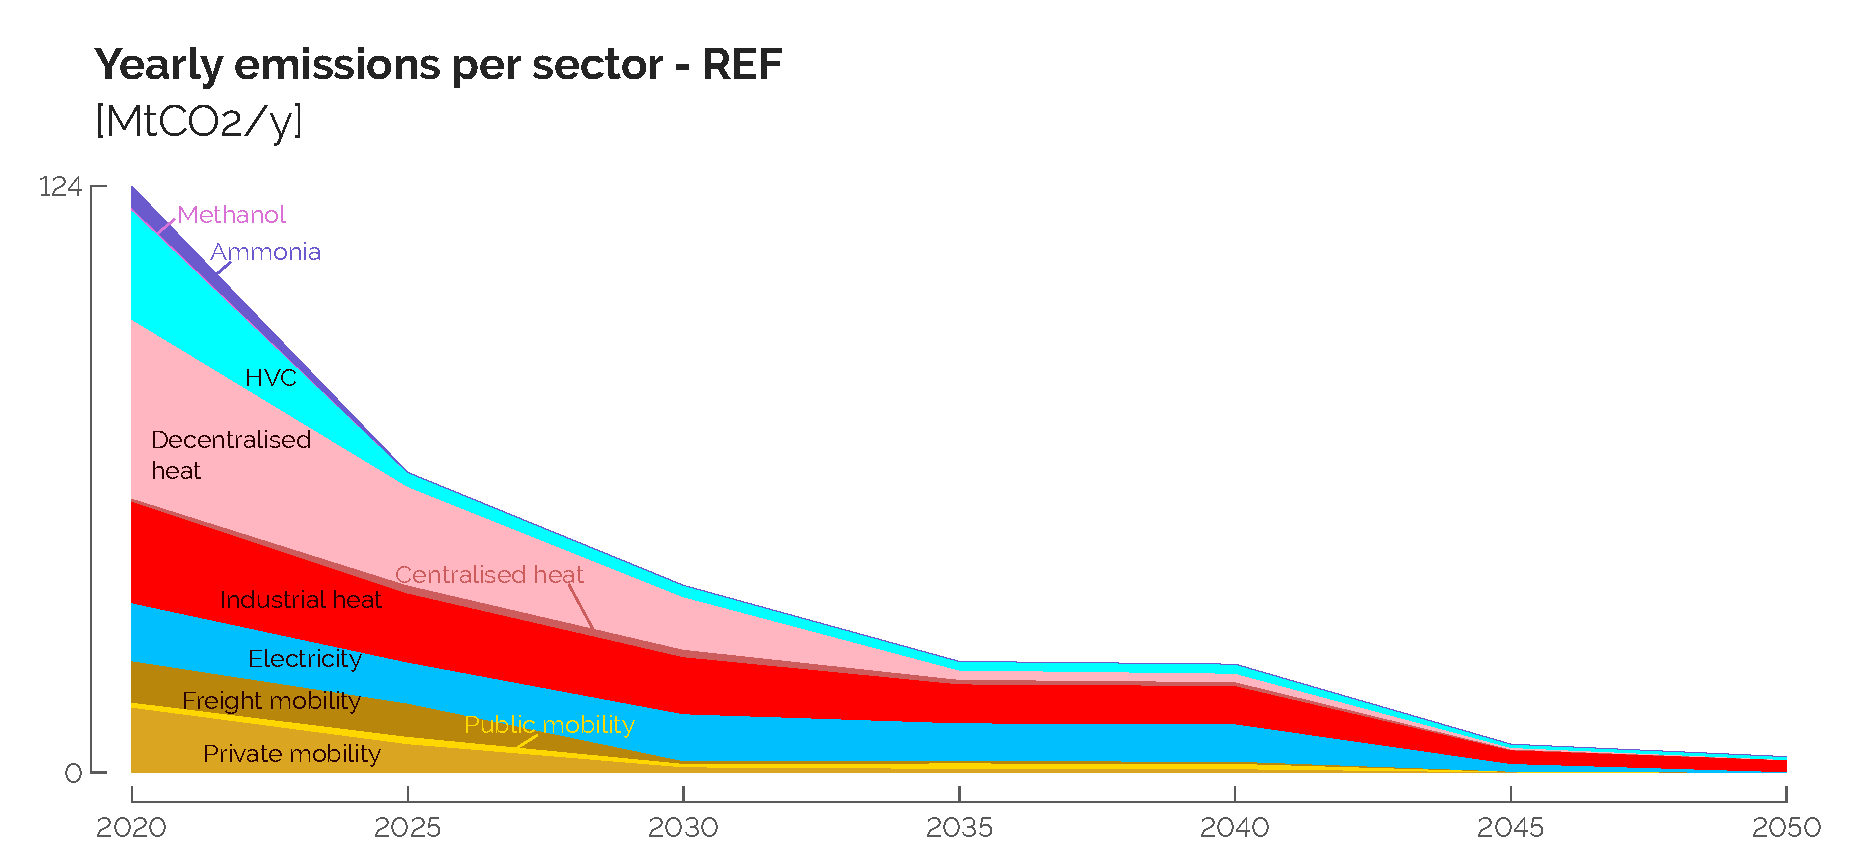
\includegraphics[width=0.49\textwidth]{GWP_per_sector_REF.pdf}
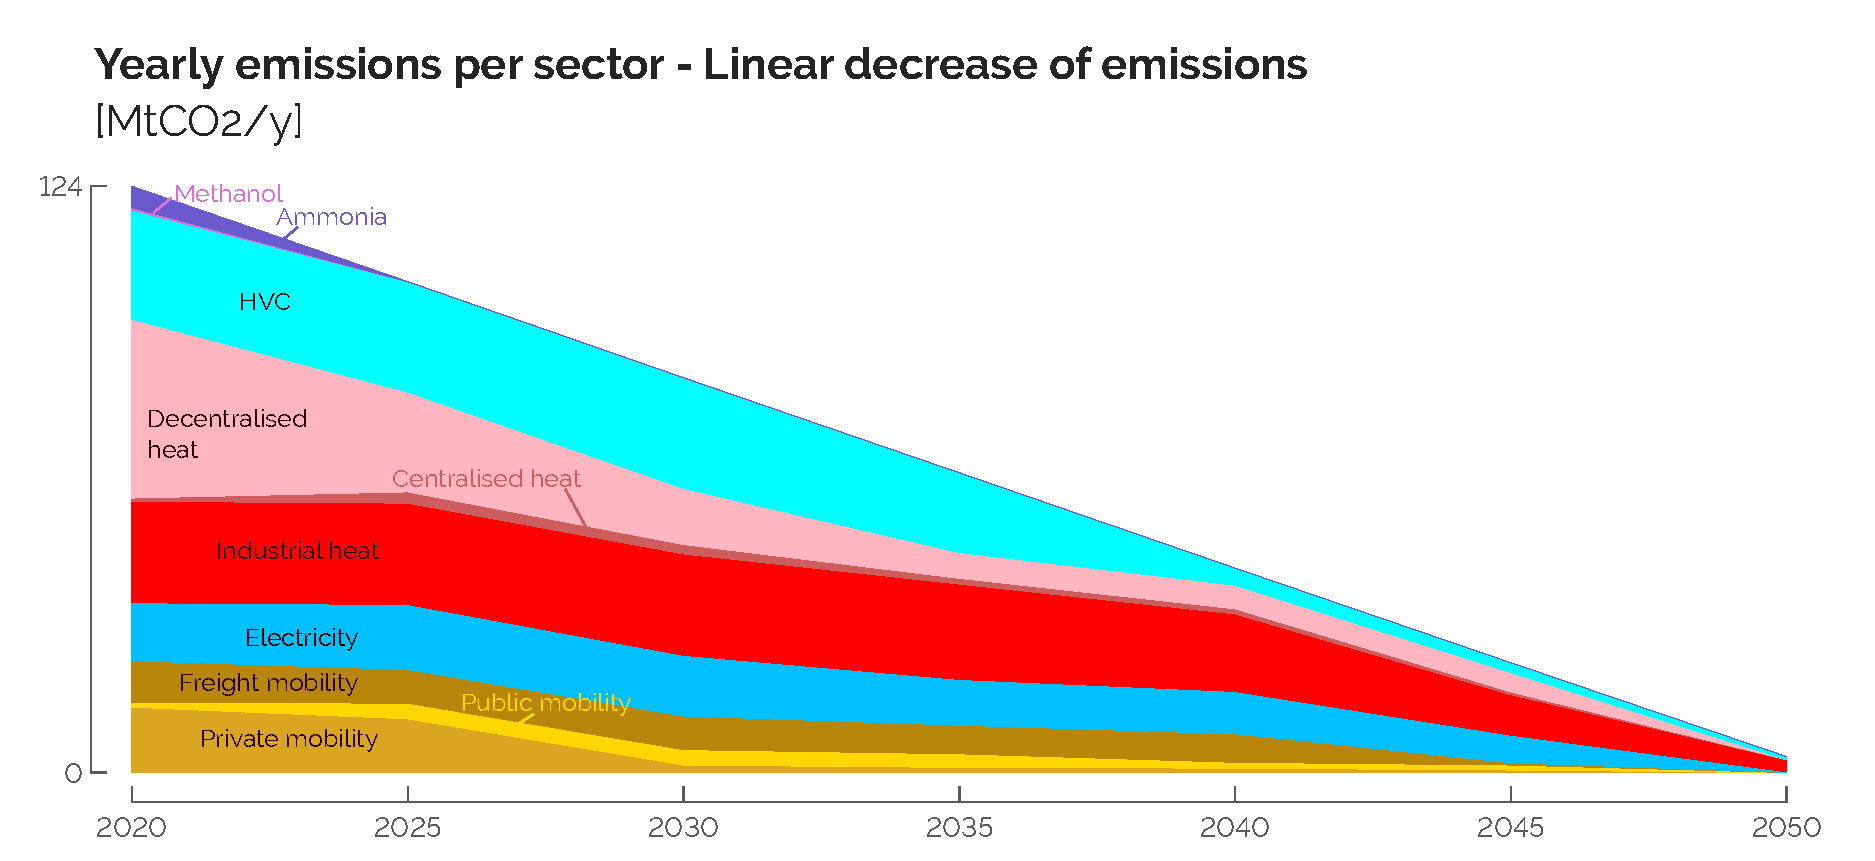
\includegraphics[width=0.49\textwidth]{GWP_per_sector_lin.pdf}
\caption{Respecting the \ce{CO2}-budget imposed in the REF case drastically cuts the emissions of the system, especially in the production of \glsxtrfull{HVC} and the high-temperature heating sector.}
\label{fig:app_CO2_REF_lin}
\end{figure}


\end{appendices}


\end{document}
